%\documentclass[spanish,a4paper,11pt,oneside,links]{report}
\documentclass[spanish,a4paper,openany,11pt]{book}
\usepackage{graphicx}
\usepackage{amsmath,amsfonts}
\usepackage[utf8]{inputenc}
\usepackage[spanish]{babel}
\usepackage[Algoritmo]{algorithm}
\usepackage{algpseudocode}
\usepackage{url}
\usepackage{fancyhdr}
\usepackage{epstopdf}


\usepackage{emptypage}

\lhead[]{\rightmark}
\chead[]{}
\rhead[\leftmark]{}
\renewcommand{\headrulewidth}{0.5pt}

\fancypagestyle{plain}{
\fancyhead[L]{}
\fancyhead[C]{}
\fancyhead[R]{}
\renewcommand{\headrulewidth}{0pt}
}

\pagestyle{fancy} 


\begin{document}


\begin{titlepage}
\begin{center}

Universidad Nacional de Rosario

Facultad de Ciencias Exactas, Ingeniería y Agrimensura

Tesis Doctoral

\vspace{2cm}


{\huge Título: TO-DO}
\vspace{2cm}

{\large Lic. Rodrigo Baravalle}
\vspace{2cm}

{\large Director: Claudio Delrieux}

{\large Co-Director: Juan Carlos Gómez}

\vspace{2cm}
{\large Miembros del Jurado: TO-DO}

\vspace{2cm}
{\large Tesis presentada en cumplimiento parcial para optar por el título de Doctor en Informática}

\vspace{1cm}
Fecha: TO-DO
\end{center}
\end{titlepage}

 \cleardoublepage

\chapter*{Agradecimientos} % si no queremos que añada la palabra "Capitulo"
\pagenumbering{Roman} % para comenzar la numeracion de paginas en numeros romanos
\addcontentsline{toc}{chapter}{Agradecimientos} % si queremos que aparezca en el índice
\markboth{AGRADECIMIENTOS}{AGRADECIMIENTOS} % encabezado 
 
¡Muchas gracias a todos!

\chapter*{Resumen} % si no queremos que añada la palabra "Capitulo"
\addcontentsline{toc}{chapter}{Resumen} % si queremos que aparezca en el índice
\markboth{RESUMEN}{RESUMEN} % encabezado

Una bonita historia
\tableofcontents % indice de contenidos

\cleardoublepage
\addcontentsline{toc}{chapter}{Lista de figuras} % para que aparezca en el indice de contenidos
\listoffigures % indice de figuras

\cleardoublepage
\addcontentsline{toc}{chapter}{Lista de tablas} % para que aparezca en el indice de contenidos
\listoftables % indice de tablas


% pagina en blanco
\newpage

\pagenumbering{arabic} 
\chapter{Introducción}
\section{Motivación}
\section{Alcances y Objetivos}
\section{Resultados Originales Presentados}

 \cleardoublepage

\chapter[Estado del Arte]{Simulación de Materiales en Computación Gráfica: Estado del Arte}
\section{Introducción} %(hablar de los diferentes materiales, cómo los modelos "fáciles" no sirven)
El renderizado en computación gráfica es el intento de producir imágenes que representan una escena tridimensional, representada por medio de primitivas matemáticas como puntos, líneas, cubos, etc..

En los últimos años, el avance en el campo del renderizado de escenas ha sido muy notorio. El nivel de realismo presente en las imágenes obtenidas ha ido en aumento hasta el punto de ser de difícil distinción para un ser humano. Dichos avances han sido, en gran parte, debido al desarrollo de dispositivos de hardware gráficos más poderosos, ya que la teoría matemática que describe el comportamiento de la luz en escenas estuvo presente desde hace varias décadas \cite{Kajiya} mediante la denominada Ecuación del Rendering.


La ecuación es una aproximación, un modelo físico que intenta describir los aspectos considerados más importantes en el fenómeno de interacción de la luz con diversos objetos en una escena.

Lamentablemente, la ecuación es, en términos teóricos, no computable. Sin embargo, el estudio a lo largo de los años de técnicas que permitan aproximarla ha dado sus frutos y ha permitido la obtención de imágenes de un realismo asombroso.

A pesar de estos increíbles avances en un corto período de tiempo, el renderizado de una escena es un problema que involucra otros inconvenientes. El más notorio de ellos, es que la ecuación del rendering no tiene en cuenta qué {\em materiales} componen los objetos que definen la escena. En otras palabras, un objeto compuesto por madera no lucirá exactamente igual que uno compuesto por metales, ni por un material orgánico compuesto de tejidos. A la par del desarrollo de técnicas de iluminación global, han surgido técnicas que han intentado abordar materiales específicos \cite{} y familias de materiales \cite{}.

Estas técnicas buscan capturar la intrincada geometría propia de cada material. Diferentes estructuras microscópicas producen distintas apariencias, reflejando la luz de distinta manera, hecho que es interpretado por la percepción humana como diferentes materiales. Por ejemplo: una superficie metálica tiene un gran componente reflexivo, emitiendo luz en direcciones bien definidas, a diferencia de una superficie más opaca como un plástico. Dado que la ecuación del rendering usa los materiales como {\em caja negra}, los mismos deben ser modelados de una manera adecuada para ser integrados en las distintas técnicas de renderizado global.

Determinados materiales han recibido mayor atención debido a su ubicuidad en escenas de películas y video juegos, o a la facilidad de su diseño: agua, fuego, aire, humo, piel humana, madera, etc. Por esta razón, las imágenes sintéticas obtenidas presentan cierta asimetría en la calidad de los distintos materiales. En contraste, otros materiales han recibido menor atención, la cual puede atribuirse a una menor presencia en escenas o a una dificultad en el modelado y visualización, la cual ha resistido las técnicas más simples.

Entre estos materiales, aquellos sometidos a un proceso de cocción han permanecido entre los más dificultosos por su compleja geometría y los fenómenos lumínicos involucrados. Tal vez el caso más emblemático de los materiales cocidos es el pan, debido a su importancia en la vida cotidiana. Como nota de color, un reconocido  científico del área, Alain Fournier, pronunció en 2001 la frase "la Computación Gráfica todavía no ha sido capaz de renderizar de manera convincente una feta de pan". En las siguientes secciones mostraremos que unos pocos intentos por abordar el problema fueron realizados pocos años después.

\section{Modelos de Geometría de Materiales}
En esta sección presentaremos distintos modelos geométricos que han hecho su aparición a lo largo de los años en computación gráfica. Los mismos son el resultado de un balance entre detalle de representación, tiempos de cómputo y recursos de memoria utilizados.

\subsection{Modelos Procedimentales}
\subsubsection{Plantas}
\subsubsection{Ciudades}
\subsubsection{Planetas}
\subsubsection{Montañas}


\subsection{Multifractal theory}

Fractal Dimensions (FD) measure key image features using few values. Different FDs capture different features, {\em e.g.}, porosity, rugosity, etc. Studies shows fractal bread characterisations using several FDs \cite{Gonzales2008,Baravalle2012}. 

Literature shows different representations for the multifractal spectrum. These representations provide identical information and differ only for a Legendre transformation. There are two main classes of multifractal spectra: generalised multifractal dimensions ($D_{q}$) and Lipschitz-H\"older exponents ($f(\alpha)$). The latter representation boosts the performance in classification tasks.

Studies compute generalised multifractal dimensions in several ways. The Sandbox multifractal method \cite{Tel1989} aims to compute the dimensions using the meaning value in a set of randomly distributed points belonging to the structure \cite{Debartolo2004}. The author defines the sandbox multifractal dimension of order q as:

 \begin{align}
D_{q\ne 1}^{sb} &= \frac{1}{q-1} \lim_{R \rightarrow 0}{
\frac{ln   { \left\langle  (M(R)/M_{0})^{q-1} \right\rangle   }}
{ln {(R/L)}       }},\\
D_{q=1}^{sb} &= \lim_{R \rightarrow 0}{
\frac{ \left\langle ln   { (M(R)/M_{0})  }  \right\rangle}
{ln {(R/L)}       }},
\end{align}

\noindent where $M_{0}$ is the white pixels count in the image binarization and  $M(R)$ is the number of points belonging to the structure in a circle of radius $R$ centered at the $i$ point. When $q\ne1$, we compute the limit as the slope of the linear fit of the values $ln(R/L)$ vs. $ ln  \left\langle  { (M(R)/M_{0})^{q-1}  }  \right\rangle$, for $R$ in $[R_{min}, R_{max}]$, where $ \left\langle   \right\rangle$ denotes mean value over sampled points. We proceed similarly when $q=1$. Computing the value for different $q \in [-Q,Q]$  we obtain the sandbox spectrum.

%The Multifractal Spectrum $f(\alpha)$ (MFS) \cite{Xu2009} applies a pixel based discrimination using pixel neighborhood information. The discrimination produces different substructures in the image characterised by a local scaling $\alpha$ exponent. The method obtains the Box FD \cite{Peitgen2004} for each structure characterised by this exponent. This produces a vector of fractal dimensions $f(\alpha)$, meaning that different fractals coexists in the structure.

%We compute the local scaling exponent $\alpha$ for every pixel in the following way: we divide the structure $E$ in disjoint substructures $E_{i}$ of size $\varepsilon$ characterised by a measure $\mu(E_{i})$, and we define the H\"older exponent, $\alpha_{i}$, for each substructure $E_{i}$, as a function of $\varepsilon$, 
 %\begin{align}
%\alpha_{i} &= \lim_{\varepsilon\to0} %\frac{ln(\mu(E_{i}))}{ln(\varepsilon)}.
%\label{eqn:eqn4}
%\end{align}
%In our case, we define $\mu$ as the image value sum in the region $E_{i}$ . We compute an $\alpha_{i}$ exponent for every pixel as the linear fit slope of the values $ln(\varepsilon)$ and $ln(\mu(E_{i}))$. We obtain the MFS computing the Box Dimension of the sub structures characterised by different $\alpha_{i}$ under different real ranges $(\alpha_{i}, \alpha_{i+1})$. For each range, the (multi) fractal dimension $f(\alpha_{i})$ of the resulting structure is:
%\begin{align}
%f(\alpha_{i}) &= -  %\lim_{\varepsilon\to0} %\frac{ln(N_{\varepsilon}(\alpha_{i}))}%{ln(\varepsilon)}.
%\end{align}
%\noindent where $N_{\varepsilon}(\alpha_{i})$is the number of points in a circle of radius $\varepsilon$ centered at the pixel with exponent $\alpha_{i}$. In practice we compute $f(\alpha_{i})$ as the (negative) slope of the linear fit between the values of $\varepsilon$ and $N_{\varepsilon}(\alpha_{i})$, for different $\varepsilon$. Computing the value for differents $\alpha_{i}$ we obtain the multifractal spectrum.

%The MFS and the sanbox spectrum are related via a Legendre Transform. We can compute the MFS using the Legendre transform of the sandbox spectrum or we can compute it directly from the underlying structure. The latter gives better classification performance. In our experiments, we use the latter approach to compute the MFS for reañ and rendered bread images, and 



\subsection{Modelos Físicos}
Desde el surgimiento del área, estos modelos han ido evolucionando gracias al incremento en el poder de cómputo del hardware gráfico disponible. Sin embargo, aún nos encontramos en los comienzos de una aplicación más difundida de los mismos.
\subsubsection{Fluídos}
\subsubsection{Telas}

\section{Representación (Renderizado)}
\subsection{Ecuación del Rendering}

\begin{equation}
EC  = REND
\end{equation}

, donde.


\subsection{BRDFs}
\subsection{Radiancia}
\subsection{Simplificaciones: Ray Tracing, Radiosity, Photon Mapping, Ray Marching, Volume Rendering }
Todas estas simplificaciones son realizadas a escala humana, es decir, sin tener en consideración la naturaleza microscópica de la luz. En esta escala, las trayectorias que describe la luz son aproximadas por líneas rectas.
\section{Materiales específicos:}
\subsection{Agua}
\subsection{Fuego}
\subsection{Humo}
\subsection{Piel}
\subsection{Otros}


\section{Conclusiones}
 \cleardoublepage
\chapter[Modelado de la Geometría de Miga de Pan]{Modelado Procedimental de Geometrías de Miga de Pan y Otros Materiales Porosos}

\section{Introducción y Motivación} % (Películas de Animación)
Como fue previamente explicado, determinados materiales recibieron menor atención en la literatura científica, debido entre otros factores, a la dificultad en el modelado, a los altos costos computacionales, y/o a la necesidad de utilización del material en aplicaciones prácticas.
Con el paso de los a\~nos, la industria del cine y de los video juegos utilizó procedimientos artísticos que intentan subsanar estas deficiencias.
De esta forma, se busc\'o la mayor similitud posible entre el material sintetizado y el real, sin importar si el proceso es una simulación física o el resultado de un procedimiento artístico.
Entre los innumerables ejemplos que se pueden citar, uno particularmente relacionado al trabajo de esta tesis lo constituye la película Ratatouille \cite{Cho2007}.
La misma se desarrolla en un ambiente de cocina, y por lo tanto existen alimentos y materiales naturales que deben ser modelados para ser renderizados.
Debido a la inexistencia de modelos estándar de determinados materiales en la literatura de computación gráfica (comestibles), los artistas y programadores encargados de llevar a cabo la producción visual de la película debieron crear técnicas ad-hoc para lograr un renderizado realista de los diferentes materiales.
Sin embargo, el éxito visual obtenido no se vio acompañado de una liberación del código que producía dichas imágenes, por lo cual la técnica permaneció para uso privado de la compañía productora, resultando en una difícil reproducción de dichos materiales por parte de terceros.

En nuestro trabajo intentamos subsanar estas deficiencias.
Por un lado, la falta de modelos ad-hoc documentados y por lo tanto reproducibles, y por otro, la utilización de modelos físicos basados en los procesos reales de formación de los materiales, los cuales sin dudas provocarán que el resultado sintético posea una mayor similitud visual y estructural a los materiales que se pretenden representar.

\section{Un Framework para la Síntesis de Texturas de Materiales}
En primer lugar presentaremos un sencillo procedimiento, en dos dimensiones, que permite obtener texturas de distintos materiales.
Dichos materiales usualmente se presentan en publicaciones separadas en la literatura, dado que los procedimientos que producen las mismas son fuertemente diferentes.
El procedimiento presentado ser\'a luego derivado para obtener texturas de pan y otros materiales porosos.

%Una vez establecidas las texturas en computación gráfica como un método simple y eficiente de representar materiales, se idearon técnicas automáticas para generarlas.
%De esta forma, no se depende exclusivamente de imágenes para obtener las mismas.

\subsection{Sistemas de Partículas y Autómatas Celulares}
En un sistema de part\'iculas \cite{Reeves1983} t\'ipico las part\'iculas nacen, se desarrollan y mueren, respetando reglas que les son impuestas por el sistema. Estos sistemas intentan modelar la din\'amica del fen\'omeno a trav\'es del tiempo, siendo uno de sus principales intereses mostrar una animaci\'on del mismo \cite{Gao2010, Bagar2010, Lentine2010}.

Se propone utilizar estos sistemas como generadores procedimentales de texturas. Un enfoque similar puede observarse en \cite{Kranidotis98}, aunque el mismo no fue desarrollado en profundidad.
Aquí se sigue una linea de investigaci\'on similar, presentando un sistema de part\'iculas que est\'a caracterizado por el crecimiento de las mismas en cada iteraci\'on, las cuales ocupan texels asign\'andoles colores, pudi\'endose detener al mismo en la iteraci\'on que se crea conveniente, obteni\'endose una textura.
Las im\'agenes resultantes presentan aleatoriedad, lo cual es deseable en materiales naturales.
A trav\'es de la direcci\'on de crecimiento de las part\'iculas se producen distintos patrones visuales.

Es posible representar materiales cl\'asicos como madera, granito y m\'armol, pero tambi\'en otros como mosaicos, pinturas, vegetaci\'on, entre muchos otros.
En un trabajo anterior \cite{Baravalle2010} se abord\'o la generaci\'on procedimental de texturas.
La diferencia radica en el mecanismo de generaci\'on, dado que con esta nueva propuesta es un {\em proceso temporal} el que produce los resultados, con lo cual puede representarse todo el proceso de formaci\'on de un material.
Adem\'as, cada corrida del algoritmo produce una textura distinta utilizando los mismos par\'ametros, debido a la naturaleza aleatoria de la generaci\'on (aunque el uso de seeding permitir\'ia repetir texturas en el caso de requerirse, por ejemplo para generar baldosas id\'enticas).

Se utiliza como plataforma de implementaci\'on a WebGL\footnote{\em http://www.khronos.org/webgl/}, recientemente propuesta por el Khronos Group (Open Standars for Media Authoring and Acceleration), dado que la misma otorga portabilidad al modelo. 
Programadores pueden incluirlo como biblioteca en aplicaciones gr\'aficas.
Dise\~nadores pueden utilizar la implementaci\'on para producir materiales, dada la intuitividad de los par\'ametros del mismo.

\subsubsection{Desarrollo}
Inicialmente el sistema consta de un conjunto de part\'iculas $P$
\begin{equation}
P = \{p_{1}, ... , p_{n}\}, n  \in \mathbb{N},
\end{equation}
uno o varios colores {\em RGB}, los cuales pueden tomar las part\'iculas.
\begin{equation}
cols = \{col_{1}, ... , col_{m} \}, m \in \mathbb{N},
\end{equation}
un conjunto de direcciones de crecimiento $D$,
\begin{equation}
D = \{d_{1}, ... , d_{k} \}, k \in \mathbb{N},
\end{equation}
y una grilla $B_{N\times N}, N \in \mathbb{N} $ de texels con colores RGB asociados (inicialmente $(R,G,B)=(0,0,0)$).

Cada elemento del conjunto $P$ posee las siguientes propiedades:
\begin{equation}
p_{i} = \{T_{i}, C_{i}, d_{i}, color_{i}\}, 1 \le i \le n,
\end{equation}
donde:

$T_{i} = \{t_{1}, ... , t_{n_{i}}\}$: conjunto de texels {\em ocupados} por la part\'icula en $B$,

$C_{i} = \{c_{1}, ... , c_{m_{i}}\}$: conjunto de texels {\em contorno} de la part\'icula en $B$,

$d_{i} \in D$: direcci\'on de crecimiento,

$color_{i}$: color {\em RGB} de la part\'icula, con ecuaci\'on \cite{Reeves1983}
\begin{equation}
color_{i} = col_{h} + rand * varcolor,
\label{eqColor}
\end{equation}

\noindent
y donde rand es un n\'umero pseudo-aleatorio uniformemente distribuido entre $-1$ y $1$, $varcolor$ un par\'ametro y $col_{h} \in cols$.
Cada $t \in T_{i}$ tiene asociado un color que var\'ia con respecto a $color_{i}$, de similar manera a la ecuaci\'on (\ref{eqColor}).

El {\em contorno} de una part\'icula determina los texels que la misma puede incorporar. 
En cada iteraci\'on, se elige aleatoriamente un texel en $C_{i}$, se lo quita del mismo y se lo incorpora a $T_{i}$.
Luego se actualiza el contorno de acuerdo a $d_{i}$ y al nuevo texel incorporado.
Se repite el proceso $\forall p_{i} \in P$, respetando las siguientes restricciones:
\begin{eqnarray}
\forall p_{i}, p_{j} \in P, t \in T_{i} \Rightarrow t \notin T_{j}, \\
\forall p_{i} \in P, t \in T_{i} \Rightarrow t \notin C_{i}.
\end{eqnarray}

Es decir, si una part\'icula posee un texel en $T_{i}$, ninguna otra lo posee (las part\'iculas son disjuntas), y si una part\'icula posee un texel en $T_{i}$, \'este no est\'a en su contorno.

Las part\'iculas pueden {\em nacer} y {\em morir}, lo cual representa su inclusi\'on o eliminaci\'on de $P$.
Al morir, la part\'icula deja asociados los colores de su conjunto $T_{i}$ en $B$, pudiendo utilizarse posteriormente esta informaci\'on.

Podemos intentar aplicar estas técnicas al modelado procedimental de texturas. 

En la Fig.~\ref{resultados} se observan algunas im\'agenes sintetizadas.
En la primera fila, la primera y cuarta textura muestran patrones con direcci\'on vertical, direcci\'on elegida para hacer crecer a las part\'iculas.
La \'ultima figura de la segunda fila, muestra part\'iculas que crecen en 3 direcciones posibles: aleatorio ($50\%$), vertical ($25\%$) y horizontal ($25\%$), lo cual demuestra que se posee un control preciso sobre las formas resultantes en las texturas.
En la Figura \ref{sintesis} se observa un ejemplo de s\'intesis.
De izquierda a derecha, se observan texturas obtenidas en las iteraciones $10$, $150$, $250$, $500$ y $1000$.
En la Figura \ref{teteras} se observan texturas sintetizadas aplicadas a un objeto mediante texture mapping, mostrando una calidad aceptable para ser utilizadas en aplicaciones gr\'aficas.
La Figura \ref{muerte} muestra el efecto de muerte de part\'iculas.
Las mismas liberan el espacio en $T_{i}$ dejando asociado su color en $B$, permitiendo que las dem\'as puedan crecer en dichos texels.
De esta forma, puede utilizarse posteriormente la informaci\'on que la misma dej\'o asociada.
En este caso los colores de la part\'icula que libera el espacio y la ocupante fueron mezclados, obteni\'endose im\'agenes que parecen haber sido ``pintadas'' por capas.
%En la Figura \ref{software} se observa el modelo corriendo en un navegador web.


\begin{figure}[t!]
\centering
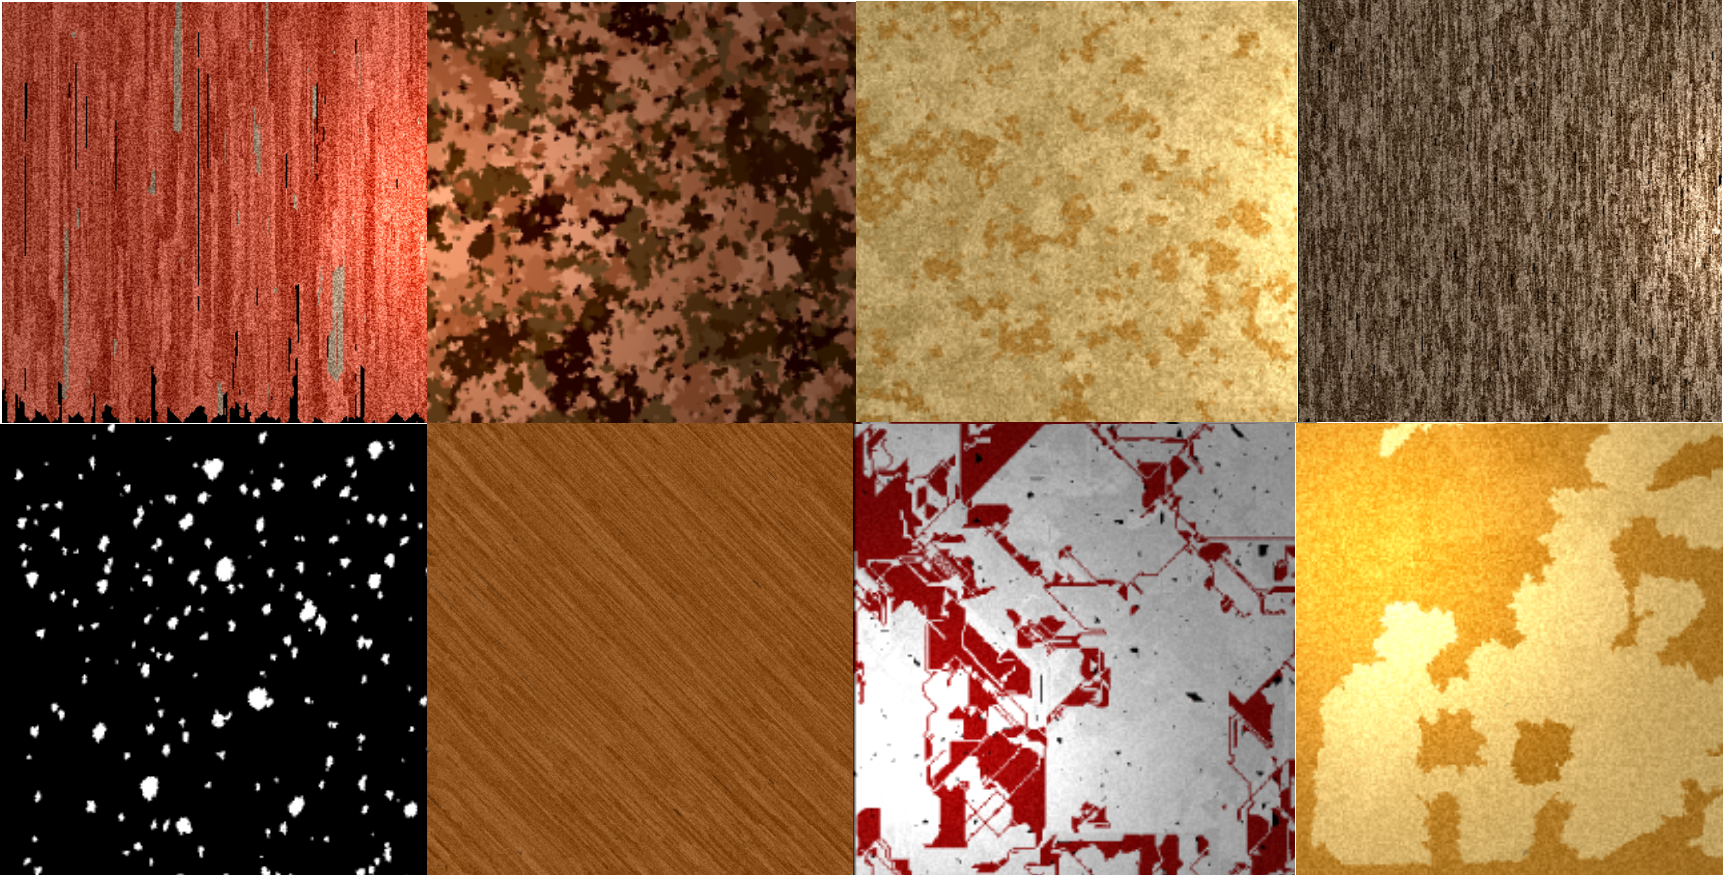
\includegraphics[scale=0.18]{resultados}
\caption{Distintas texturas obtenidas}
\label{resultados}
\end{figure}

Se muestra un ejemplo de s\'intesis de una textura en la Figura \ref{sintesis}. Deben seleccionarse los siguientes par\'ametros:

\begin{itemize}
\item Par\'ametro {\em cantidad de part\'iculas iniciales}, con valor $100$.
\item Par\'ametro {\em nuevas particulas por iteraci\'on}, con valor $1$.
\item Par\'ametros {\em color 1 y 2 (RGB)}. con colores de ejemplo, uno con la componente verde mayor y otro con mayor componente azul.
\item Par\'ametros {\em direcciones}: aleatorio: $50\%$, diagonal $50\%$.
\item Par\'ametro {\em variaci\'on de color}, con valor 0.1, en una escala [0,1] (ver $varcolor$ en la secci\'on anterior).
\item Par\'ametro {\em variaci\'on de color por part\'icula}, con valor 0.1, en una escala $[0,1]$, el cual determina la variaci\'on del color por texel dentro de la part\'icula.
\end{itemize}

\begin{figure}[t!]
\centering
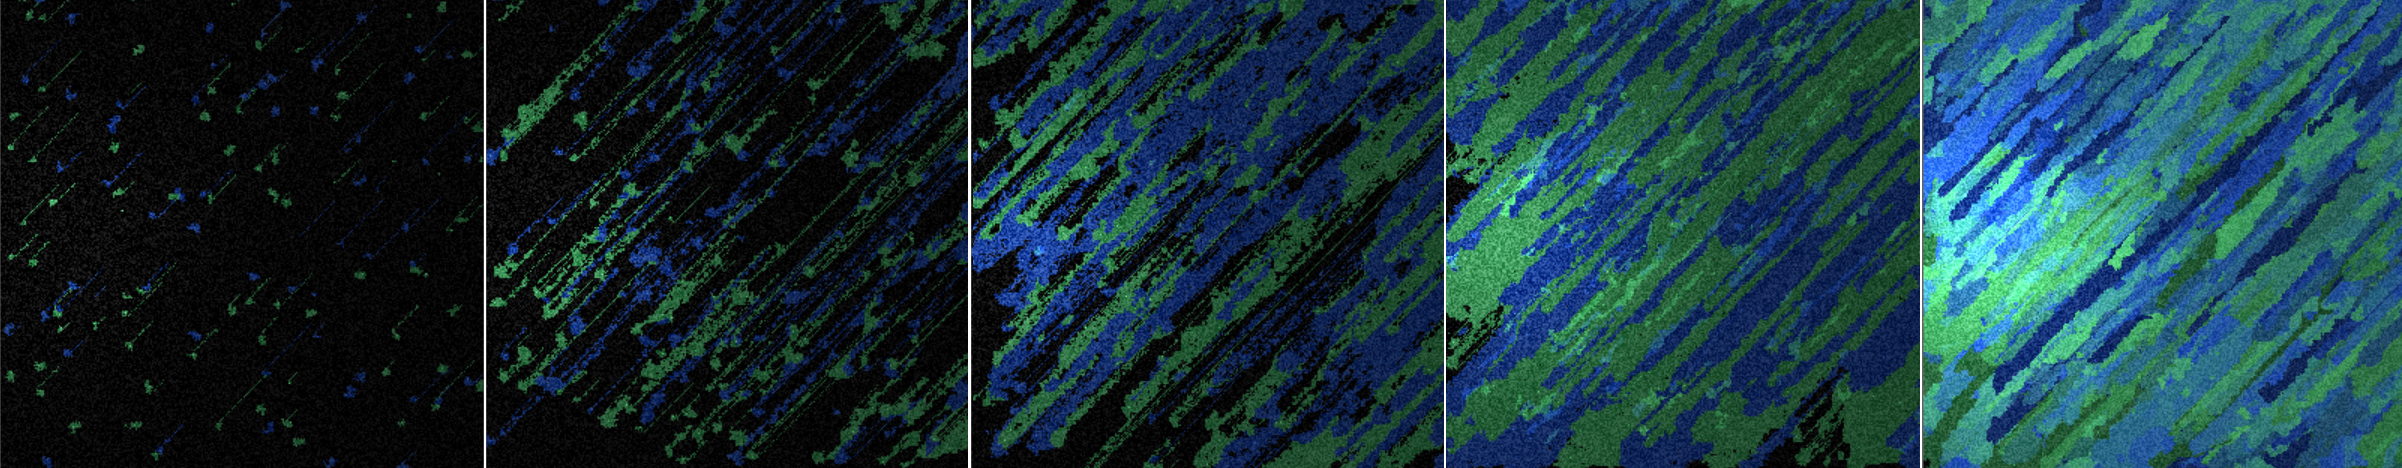
\includegraphics[scale=0.12]{sintesis}
\caption{Ejemplo de s\'intesis de una textura}
\label{sintesis}
\end{figure}

\begin{figure}[t!]
\centering
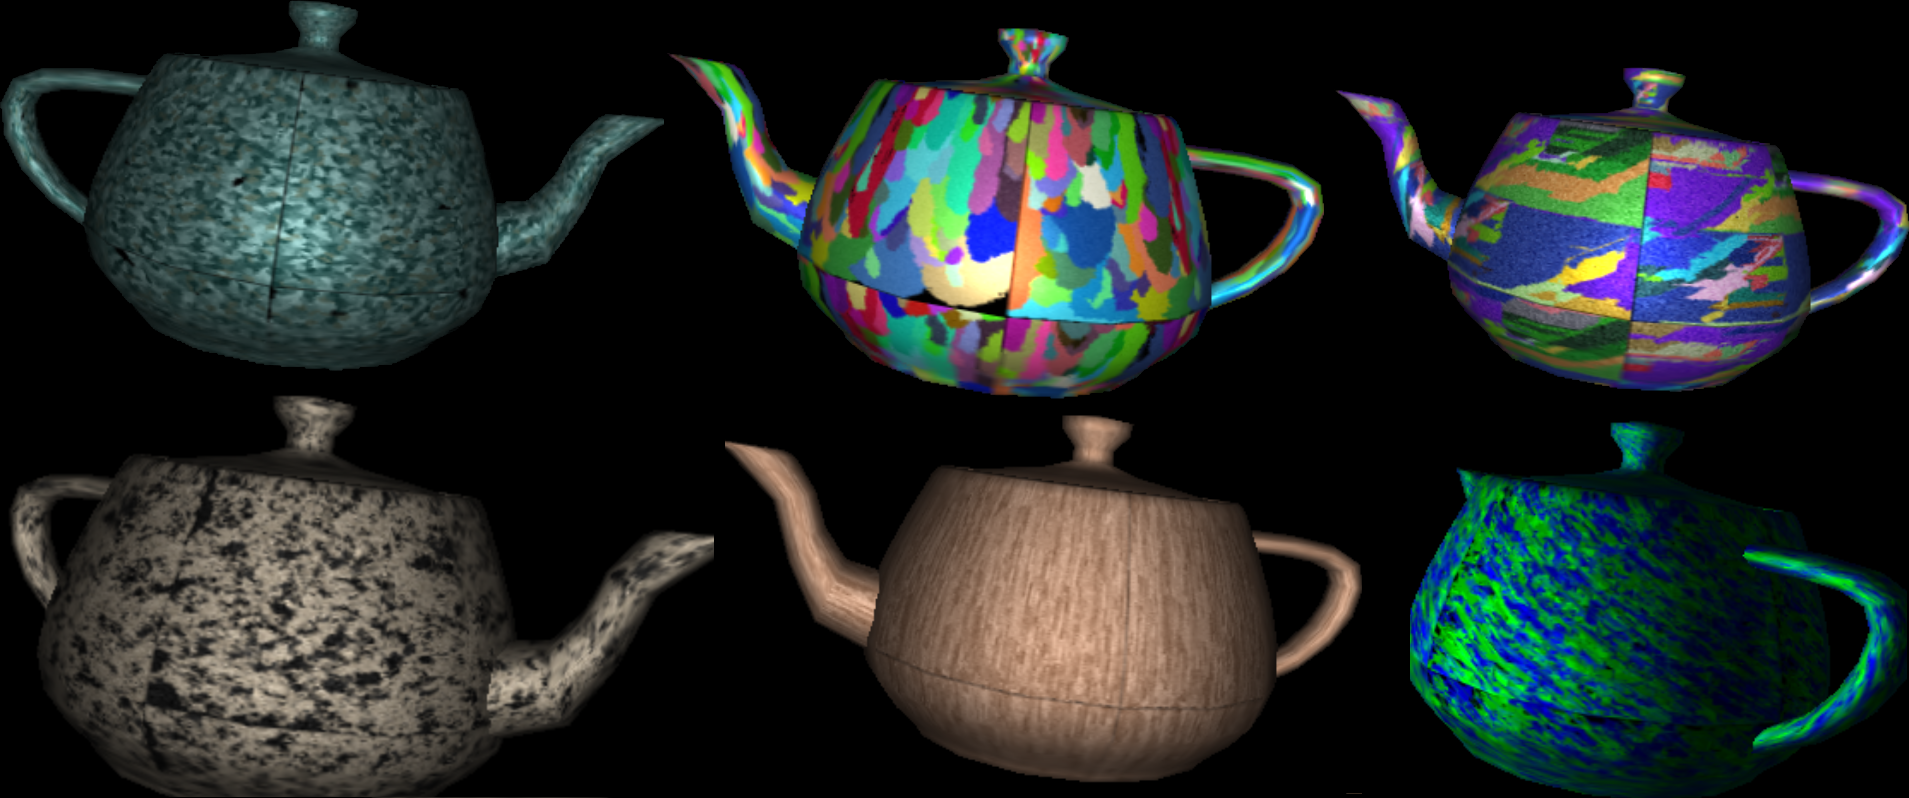
\includegraphics[scale=0.14]{teteras}
\caption{Texturas generadas mapeadas en una tetera}
\label{teteras}
\end{figure}


\begin{figure}[t!]
\centering
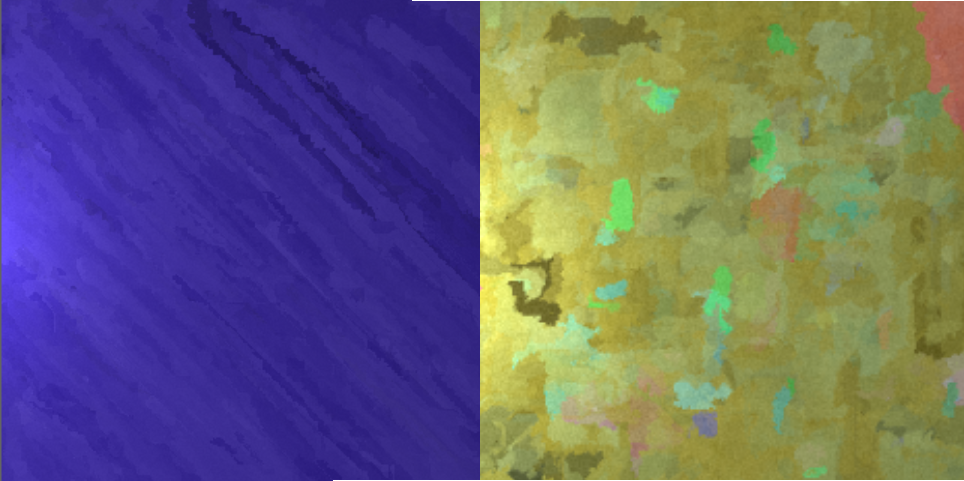
\includegraphics[scale=0.2]{muerte}
\caption{Efecto producido utilizando el concepto de muerte de las part\'iculas}
\label{muerte}
\end{figure}

Los resultados obtenidos muestran una flexibilidad útil para producir distintos materiales.
La idea de utilizar sistemas de partículas para producir materiales será utilizada en la sección siguiente.
Más específicamente para producir geometrías de materiales porosos, particularmente la miga de pan.
Para esto, se generalizarán los resultados a tres dimensiones.

\section{Modelado Procedimental de la Geometría de la Miga de Pan}
En esta sección introducimos un modelo procedimental que permite realizar simulaciones de la geometr\'ia de la miga de pan, basado en el framework introducido en la secci\'on anterior.
Si bien el modelo introducido no está basado en primeros principios, el mismo es un paso previo que permite sentar las bases de un modelo inspirado físicamente.

\subsection{Introducción}
La inmensa variedad de materiales, y sus complejas interacciones con fuentes lumínicas, han sido un tópico central de investigación en las últimas décadas en Computación Gráfica.
El modelado de la naturaleza en física ha demostrado capturar de manera muy precisa fenómenos de transporte de la luz.
Las aproximaciones computacionales a estos modelos son una de las ramas más investigadas en el renderizado de materiales.
El modelado geométrico de materiales sigue una estrategia de investigación similar. Primero se construye un modelo físico del material, el cual luego es aproximado computacionalmente.
Debido a estas observaciones, el renderizado foto-realístico de materiales debe considerar tanto el modelado geométrico de los mismos como su interacción con la luz, para lograr una aproximación adecuada del material.

La elección del modelo geométrico depende de cada material, y de la escala de representación buscada.
Esta elección influencia fuertemente el algoritmo de renderizado. 
Existen dos tipos principales de modelado de materiales: superficies y volúmenes.
Para esto existen dos ecuaciones principales.
Por un lado, la ecuación del rendering \cite{Kajiya1986} captura la microgeometría de los materiales y su interacción con la luz en superficies.
Por otro, la ecuación del rendering de volúmenes \cite{Kajiya1984} modela fenómenos volúmetricos como la transmitancia, la extinción, etc., debido a propiedades del medio (o material).

Si el material a representar es homogéneo (metales, plásticos, y similares), la elección típica es utilizar una superficie para representar el mismo \cite{Neumann1999}.
Esta elección modela la superficie del material asumiendo distribuciones estadísticas en su microgeometría.
Para lograr capturar detalles mesoscópicos, por ejemplo en el caso de maderas o ladrillos \cite{Lefebvre2000}, una técnica usual es precomputar dichas características en texturas, las cuales luego son mapeadas en la superficie.
La utilización de superficies es usualmente menos costosa computacionalmente, pero por otro lado impone limitaciones al realismo que se puede alcanzar, sobre todo en aquellos detalles que son propios de la estructura a nivel mesoscópico y la interacción de la misma con la luz (por ejemplo luz que pasa a través de agujeros en una superficie).

Siguiendo este razonamiento, la miga del pan es un material extremadamente complejo de capturar, modelar y renderizar, debido a la geometría a distintos niveles (microscópico y mesoscópico) y su resultante interacción y fenómenos lumínicos.
De esta forma, la utilización de superficies no es adecuada bajo ningún punto de vista, ya que la textura del pan está dada en gran medida por los fenómenos previamente explicados.
Si bien es cierto que existen métodos en la literatura que utilizan superficies para representar características mesoscópicas de los materiales como funciones de texturas bidireccionales (bidirectional texture functions, BTF) \cite{Tong2002}, las mismas no manejan adecuadamente la interacción lumínica antes mencionada.
Existe un intento en la literatura por suprimir esta falta \cite{Tong2005}.
El método produce imágenes realistas, pero existen muchas dificultades prácticas en la captura, el cómputo y el renderizado.
Estas limitaciones provocan que la utilización de dicho método no sea práctica por el momento.
Además, el método resulta inflexible dado que para cada imagen del material es necesario repetir todo el proceso (dos imágenes distintas del material requieren dos capturas).
Tampoco es posible obtener cortes del mismo, dada la naturaleza de superficie del método.

Por otro lado, existen numerosas publicaciones que tratan el modelado de materiales mejor adaptados a una representación volumétrica (por ejemplo humo o nubes) \cite{Chentanez2011,Zhou2008}.
La utilización de volúmenes es costosa computacionalmente pero presenta varias ventajas. Una de ellas es que no depende de una malla de triángulos, como en el caso de las superficies, y por lo tanto no presenta las desventajas mencionadas para las mismas.

Finalmente, existe una elección al momento de modelar materiales complejos y elegir una representación adecuada.
Donde se requiere simplicidad y velocidad (posiblemente tiempo real), se utilizan superficies, en cambio, si el foto-realismo es el objetivo final, es más adecuado optar por una representación volumétrica.
En los últimos años esta elección se ve perturbada por la aparición de hardware paralelo de alta velocidad (placas gráficas o GPUs), ya que un diseño adecuado podría alcanzar imágenes foto-realistas utilizando volúmenes en tiempos interactivos.
Esto es lo que presentaremos a continuación.


En este trabajo proponemos una representación volumétrica para la geometría de la miga de pan, alcanzando incluso tasas de refresco de tiempo real.
Existe un intento similar en la literatura \cite{Perlin1989}, el cual utiliza funciones algebraicas que representan la geometría del material.
En nuestro caso, para ganar flexibilidad de diseño, utilizamos los sistemas de partículas previamente mencionados, en un cubo (tres dimensiones), en conjunto con sistemas dinámicos \cite{Strogatz2001} que provocan una evolución del sistema, produciendo patrones con formas geométricas naturales.
Este es un intento por simular el efecto de la levadura en la masa cruda del pan.
Estos procedimientos producen distribuciones de burbujas de distintos tamaños, resultando en un mecanismo controlable, que presenta propiedades estadísticas.
El sistema es capaz de generar imágenes foto-realistas de diversos tipos de pan, como se mostrará más adelante.

\section{Sistemas Dinámicos como Modelo de Miga de Pan}
El prop\'osito de este algoritmo es producir una geometr\'ia la cual se renderizar\'a posteriormente. Por lo tanto, en lugar de devolver el color de una posici\'on espec\'ifica, el algoritmo genera un campo escalar compuesto de $0$s y $1$s ($0$ si la posici\'on contiene aire, $1$ si la misma contiene masa).
Esta representaci\'on resulta adecuada para ser renderizada utilizando DVR.

El sistema consta de un conjunto de part\'iculas $P$,

\begin{equation}
  P = \{p_{1}, ... , p_{n}\}, n  \in \mathbb{N},
\end{equation}

\noindent una grilla $L_{N\times N \times N}, N \in \mathbb{N} $ (inicialmente $L_{xyz}=1$) de masa y aire como fue descripto previamente, y otra grilla $L^{2}_{N\times N \times N}$, (inicialmente $L^{2}_{xyz}=-1$) de posiciones donde cada celda almacena un único entero que indica qu\'e part\'icula es due\~na de la misma ($i$ si el elemento de la grilla pertenece al contorno o interior de la part\'icula $i$).

Cada elemento en $P$ posee las siguientes propiedades:

\begin{equation}
  p_{i} = \{O_{i}, C_{i}\}, 1 \le i \le n,
\end{equation}

\noindent donde:

\begin{itemize}
\item $O_{i} = \{o_{1}, ... , o_{n_{i}}\}$: (Ocupadas) vector (conjunto) de posiciones ocupadas por la part\'icula en $L$.

\item $C_{i} = \{c_{1}, ... , c_{m_{i}}\}$: (Contorno) vector (conjunto) de posiciones representando el {\em contorno} de la part\'icula en $L$.
\end{itemize}

El vector $O$ representa las posiciones que ser\'an afectadas por la part\'icula, y el contorno $C$ se utiliza para asegurar que las part\'iculas se eviten entre s\'i.

El algoritmo se describe, simplificadamente, en Algoritmo $1$. 

\begin{algorithm}[h!]
\caption{Algoritmo de modelado}
\begin{algorithmic}

\State{$t  = 0$}
\Comment{tiempo - iteración}
\State{$P  = []$}
\Comment{partículas}
\State{$L  = matriz(MxMxM).valores\_iniciales(1)$}
\Comment {Geometría - iniciada a 1 (masa)}
\State{$L^{2} = matriz(MxMxM).valores\_iniciales(-1)$}
\Comment{Dominio de cada partícula}

\For{$i \in [1,Cantidad\_Particulas]$}
    \Comment{Cada partícula toma una posición aleatoria en L}
    \State{$x \gets aleatorio, y \gets aleatorio()$}
    \State{$O[i] \gets [[x,y]]$}
    \State{$C[i] \gets []$}
    \For{$v \in vecindario(x,y)$}
        \State{$C[i].agregar(v)$}
    \EndFor
    \State{$P.agregar([O[i],C[i]])$}
\EndFor

\For {$t \in [0,tiempo\_max]$}
    \For {$i \in [1,Cantidad\_Particulas]$}
        \If {$vacio?~C[i]$}
            \State{morir()}
        \EndIf
        \For{$h \in C[i]$}
            \State{$C[i].eliminar(h)$}
            \Comment{la posición ya fue explorada}
            \State{// Si la posición o el contorno pertenece a otra partícula, elegir otra posición}
            \State{// borde\_libre chequea que el vecindario no este dominado por otra partícula}
            \If{$!(L^{2}[h] > 0 ~\&\&~ L^{2}[h] != i ~\&\&~ borde\_libre(separacion)$}
                \State{// Posición libre, ocupar}                
                \State{$L[h] \gets 0$} \Comment{masa -> aire}
                \State{$O[i].agregar(h)$}
                \State{$C[i].agregar(vecindario(h))$} 
                \State{$L^{2}.setear(vecindario(h),i)$} \Comment{Marcar posiciones en $L^{2}$ como $i$}
                \State{$L^{2}.setear(h,i)$}
                \Comment{turno de la particula $i+1$...}
            \EndIf
        \EndFor
    \EndFor
\EndFor
\end{algorithmic}
\end{algorithm}

Cuando $t = 0$, un conjunto de part\'iculas iniciales toman posiciones aleatorias en la grilla. Para cada partícula, la posici\'on elegida es la primera posici\'on ocupada en $O$, adem\'as, el vecindario de $O$ es agregado a $C$. Cada part\'icula evoluciona en un intento por extender sus posiciones ocupadas ($O$), marcando posiciones en $L$. Las posiciones se toman de $C$. Cuando una part\'icula ocupa una posici\'on, la misma se elimina de $C$ y se agrega a $O$. Luego el vecindario de esa posici\'on se agrega a $C$ (es decir las posiciones que rodean inmediatamente a la posici\'on tomada). Las grillas se actualizan de la siguiente manera: $L$ se setea a $0$ en la posici\'on y $L^{2}$ se setea con el valor $i$ en las posiciones que se agregan a $C$. Las part\'iculas s\'olo pueden crecer si el valor encontrado en $L^{2}$ no pertenece a otra part\'icula. El tama\~no del vecindario es un par\'ametro que define la distancia entre part\'iculas. Si el vector $C$ est\'a vac\'io, la part\'icula {\em muere} ya que no puede continuar creciendo.


El algoritmo puede ser terminado en cualquier $t$ deseado. El mismo puede finalizar su c\'omputo ante determinados eventos, por ejemplo, cuando todas las posiciones de $L^{2}$ fueron tomadas por part\'iculas, ya que no pueden realizarse progresos.

Variando el par\'ametro de distancia entre part\'iculas (separación) se obtienen distintas estructuras (ver Fig.~\ref{fg:sistdin1}). Las im\'agenes muestran ejemplos 2D (para mayor claridad) de crecimiento aleatorio de part\'iculas. La regi\'on blanca en las im\'agenes representa la masa restante luego del proceso.


\begin{figure*}[htb!]
  \centerline{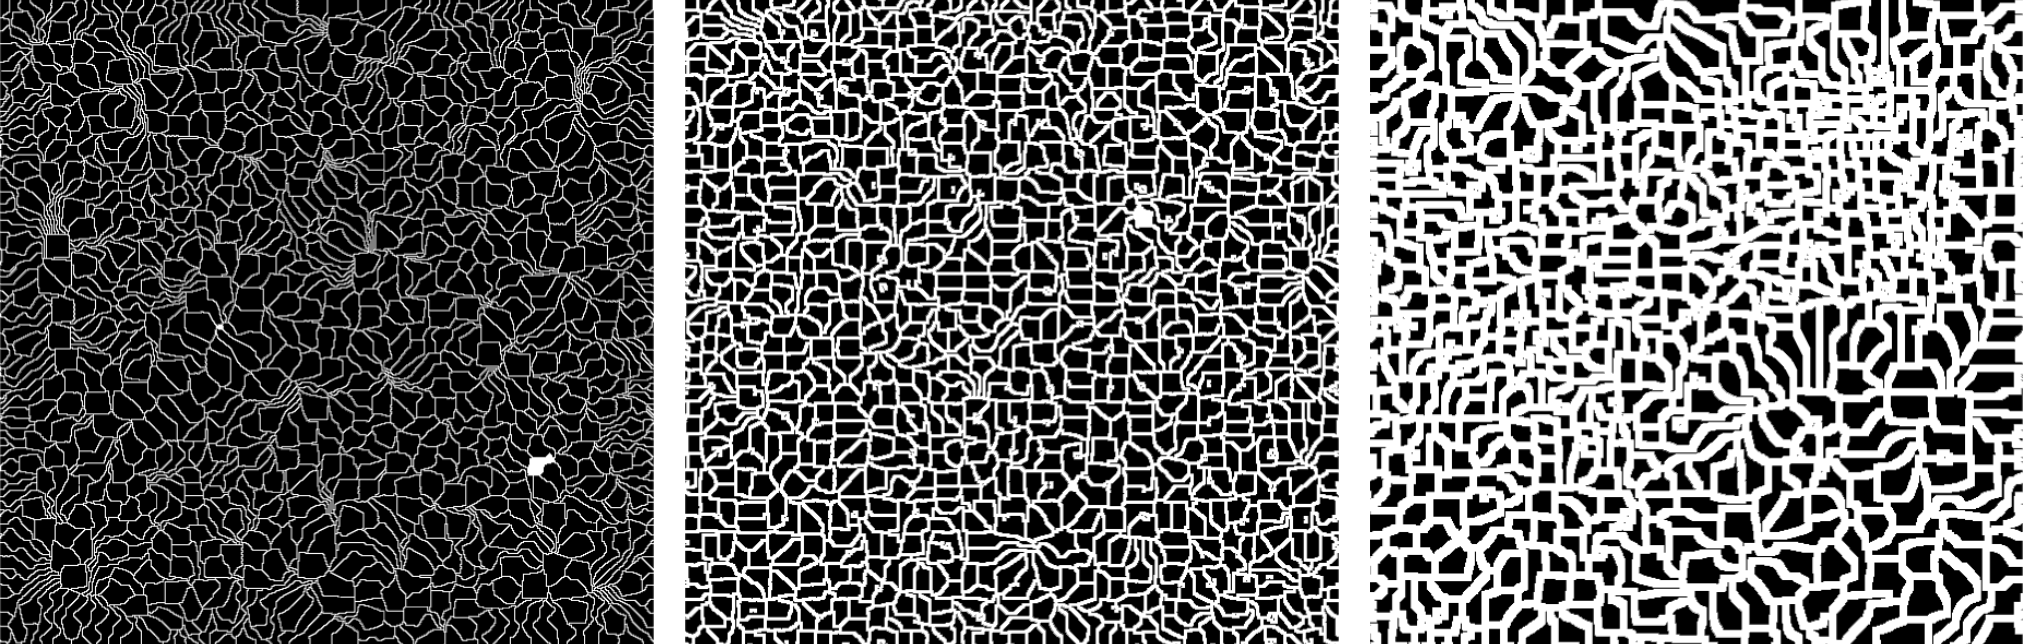
\includegraphics[width=13cm]{sistdin1}}
  \caption{Diferentes separaciones entre part\'iculas utilizando el par\'ametro separación. Izquierda: separaci\'on = 1, centro: separaci\'on = 2, derecha: separaci\'on = 4.}
  \label{fg:sistdin1}
\end{figure*}

Finalmente, el algoritmo devuelve la grilla $L$, la cual ser\'a renderizada posteriormente. En la siguiente secci\'on se explica la utilizaci\'on de sistemas din\'amicos en la evoluci\'on guiada de part\'iculas.

\subsection{Sistemas Din\'amicos}

Las ecuaciones diferenciales tienen como prop\'osito tratar con la dificultad (o imposibilidad) de hallar soluciones anal\'iticas en procesos din\'amicos. En primer lugar, se define un modelo matem\'atico del problema, del cual luego se obtienen 
las ecuaciones diferenciales asociadas. Los mismos se resuelven por medio de aproximaciones num\'ericas en cada instante de tiempo.

Los costos computacionales de estas soluciones dependen de la complejidad del problema y el n\'umero de ecuaciones del sistema. En este trabajo proponemos utilizar una sub-\'area de ecuaciones diferenciales llamada ecuaciones diferenciales ordinarias (ODE). En esta representaci\'on, el tiempo es tratado como la \'unica variable independiente.


De manera general, las ODEs se representan utilizando el siguiente sistema de ecuaciones:
\begin{equation} \label{eq:simple}  
  \begin{aligned}
    \dot{x_{1}} = f_{1}(x_{1},\ldots,x_{n}),\\
    \ldots\\
    \dot{x_{n}} = f_{n}(x_{1},\ldots,x_{n}),
  \end{aligned}
\end{equation}

\noindent donde $\dot{x_{i}}$ representa la derivada de $x_{i}$ con respecto
a $t$. Las variables $x_{i}$ y las funciones $f_{i}$ se definen de manera diferente para cada problema. En este caso, cada variable representa una coordenada cartesiana en el espacio, $x_{1}$ es $x$, $x_{2}$ es $y$ y $x_{3}$ es $z$. El conjunto de $f_{i}$ ser\'a definido tratando de capturar la estructura interna del pan. La siguiente secci\'on muestra cómo estos sistemas pueden describir la evoluci\'on de los sistemas de part\'iculas.

\subsection{Evoluci\'on de sistemas de part\'iculas utilizando sistemas din\'amicos}

La percepci\'on humana puede detectar patrones en la estructura de la miga de pan. Distintas observaciones pueden realizarse sobre la distribuci\'on de las burbujas en la misma (ver Fig.~\ref{fg:panreal}). Primero, la forma de las burbujas cercanas a la corteza tiende a estirarse paralelamente a la misma. Esto es resultado de la acci\'on de las elevadas temperaturas durante la cocci\'on de la masa. Tambi\'en resulta evidente que la estructura completa es similar a un fluido con la forma de la corteza.


\begin{figure*}[htb!]
  \centerline{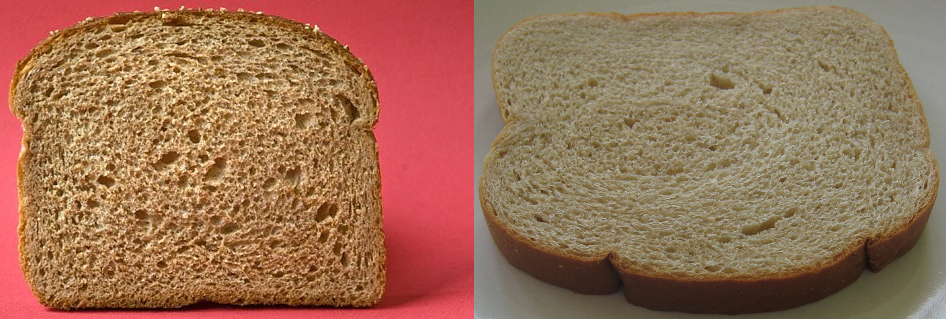
\includegraphics[width=13cm]{panreal}}
  \caption{Im\'agenes de cortes reales de pan}
  \label{fg:panreal}
\end{figure*}

Por otro lado, los sistemas din\'amicos previamente presentados producen formas naturales (ver Fig.~\ref{fg:sistdin2}). En las im\'agenes pueden observarse c\'irculos y espirales, entre otras formas. Las im\'agenes se obtuvieron dibujando trayectorias sobre un plano, siguiendo distintas ODEs. Tres ODEs describen las din\'amicas presentes en las im\'agenes. A modo de ejemplo, la imagen de la izquierda es el resultado del siguiente conjunto de ecuaciones:

\begin{equation} \label{eq:simple}  
  \begin{aligned}
    \dot{x} &= x^{2}-y^{2}+1,\\
    \dot{y} &= 2xy+1.
  \end{aligned}
\end{equation}


\begin{figure*}[htb!]
  \centerline{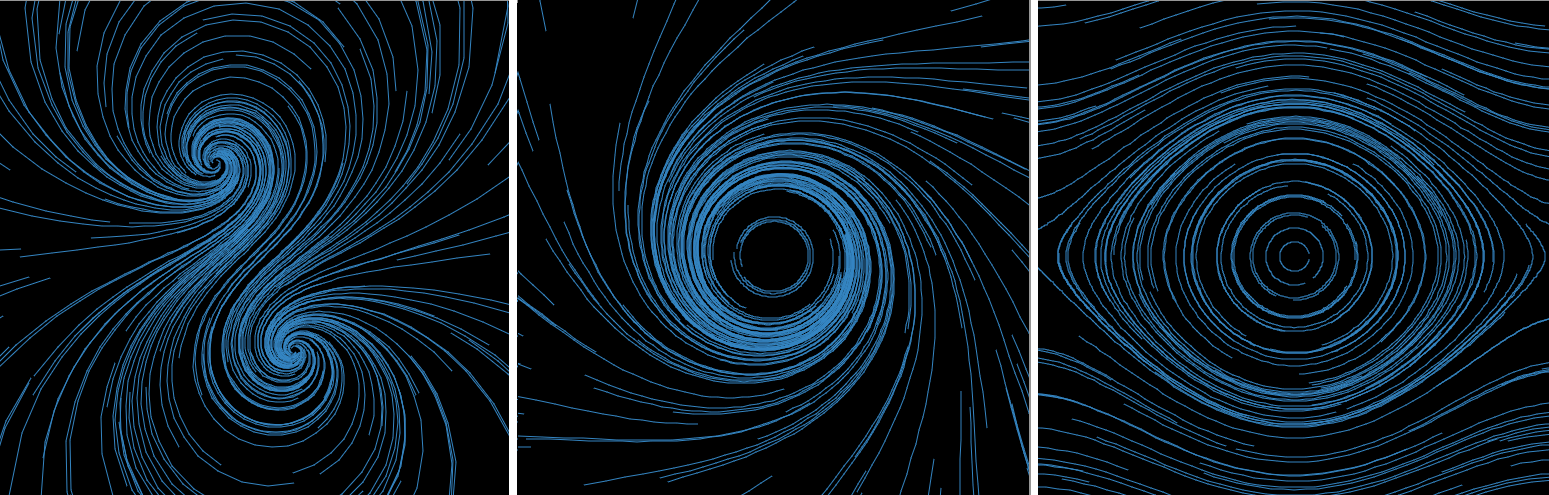
\includegraphics[width=13cm]{sistdin2}}
  \caption{Sistemas din\'amicos en el plano.}
  \label{fg:sistdin2}
\end{figure*}

En los ejemplos se eligen posiciones aleatorias y luego el sistema se resuelve por medio de un {\em solver} Runge-Kutta de cuarto orden, el cual permite conocer la direcci\'on a tomar en cada punto por la trayectoria (en las im\'agenes se computaron trayectorias hacia adelante y hacia atrás en el tiempo para lograr una mejor visualizaci\'on). La imagen de la izquierda muestra un atractor y un repeledor claramente visibles. El centro de la espiral m\'as a la izquierda es un atractor (a medida que $t$ avanza, las trayectorias convergen hacia el punto), mientras que el otro centro es un repeledor. Los atractores pueden no ser puntuales, como muestran las restantes dos im\'agenes. La imagen de la derecha muestra atractores en forma de c\'irculos (las trayectorias ciclan por el c\'irculo).

Las part\'iculas producen distintos patrones al seguir las trayectorias definidas en el plano y el espacio. Esto se logra resolviendo num\'ericamente el sistema din\'amico en la posici\'on agregada a la part\'icula, seleccionando como siguiente posici\'on de crecimiento aquella posici\'on del contorno que mejor aproxima la soluci\'on del sistema din\'amico (para esto, sólo se agrega al contorno esa posición). El Algoritmo $2$ muestra cómo se modifica el algoritmo de modelado para incluir este comportamiento.

\begin{algorithm}[h!]
\caption{Modificación del algoritmo de modelado por medio de sistemas dinámicos}
\begin{algorithmic}
\State $L[h]\gets 0$ \Comment{masa $\rightarrow$ aire}
\State $O[i].agregar(h)$
\State $solucion \gets Runge\_Kutta(h)$
\Comment {Se calcula la siguiente posición}
\State $vec = vecindario(h)$
\State $mejor = abs(vec[0] - solucion)$
\State $elegida = h$
\State $vec.eliminar(h)$
\For {$w \in vec$}
\State{// Se calcula la posición del vecindario que mejor aproxima al sistema}
    \If {$abs(vec[w]-solucion) < mejor$}
        \State $mejor = abs(vec[w]-solucion)$
        \State $elegida = w$
    \EndIf
    \If {$aleatorio() > 1-aleatoriedad$} 
    \Comment {$0 <= aleatorio() <= 1$}
        \State $C[i].agregar(w)$
    \EndIf
\EndFor
\State{// Se agrega al vecindario sólo la posición que mejor aproxima la solución}
\State $C[i].agregar(elegida)$
\end{algorithmic}
\end{algorithm}

Las part\'iculas se deforman de forma global en un patr\'on que es visualmente similar a las trayectorias que produce el sistema (ver Fig.~\ref{fg:sistdin3}). En las im\'agenes, de izquierda a derecha se decrementa la {\em aleatoriedad} de las trayectorias. El par\'ametro aleatoriedad seteado a $0.1$ genera la imagen de la derecha, lo cual significa que las burbujas eligen como siguiente posición de crecimiento la que mejor se acopla al sistema con una probabilidad de $0.9$. La probabilidad se define como $1-aleatoriedad$, donde $0 \leq aleatoriedad \leq 1$. Las ecuaciones del sistema son las mismas que las de la imagen derecha mostrada en la Fig.~\ref{fg:sistdin2}. Estos patrones pueden ser utilizados adem\'as en otros materiales cocidos, variando el par\'ametro de aleatoriedad. Distintos sistemas de ecuaciones pueden utilizarse para definir distintos patrones.

\begin{figure*}[htb!]
  \centerline{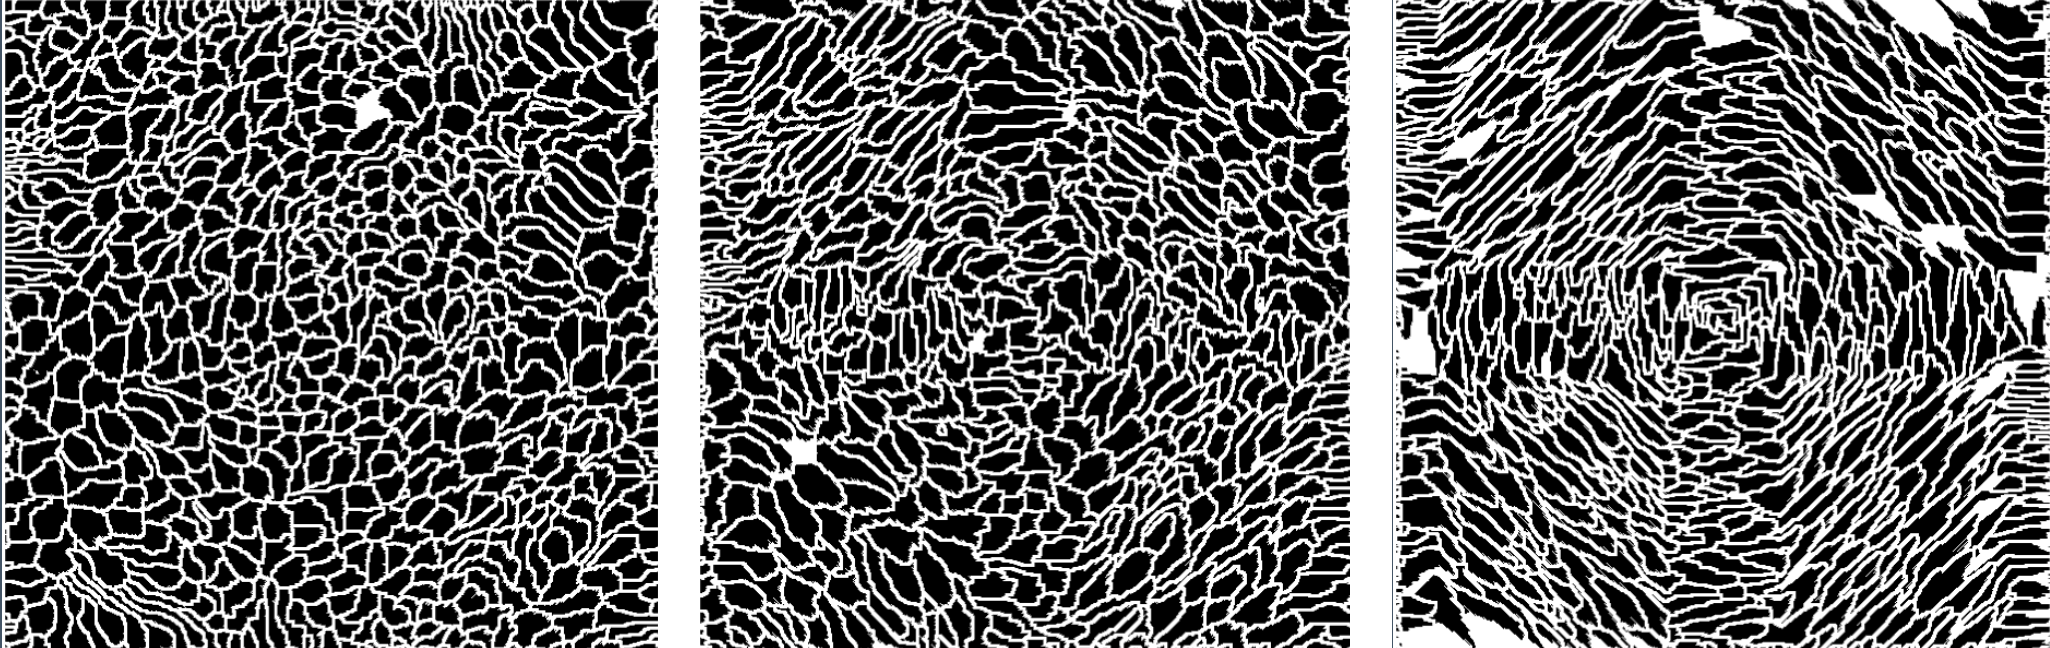
\includegraphics[width=13cm]{sistdin3}}
  \caption{Sistemas din\'amicos aplicados en sistemas de part\'iculas. Efecto del parámetro {\em aleatoriedad}. De izquierda a derecha, aleatoriedad: 0.3,0.2,0.1 respectivamente. }
  \label{fg:sistdin3}
\end{figure*}

\subsection{Resultados y Limitaciones}
Las Figs.~\ref{fg:crumb} y \ref{fg:results2} muestran imágenes renderizadas utilizando el procedimiento descrito.

\begin{figure}
  \centerline{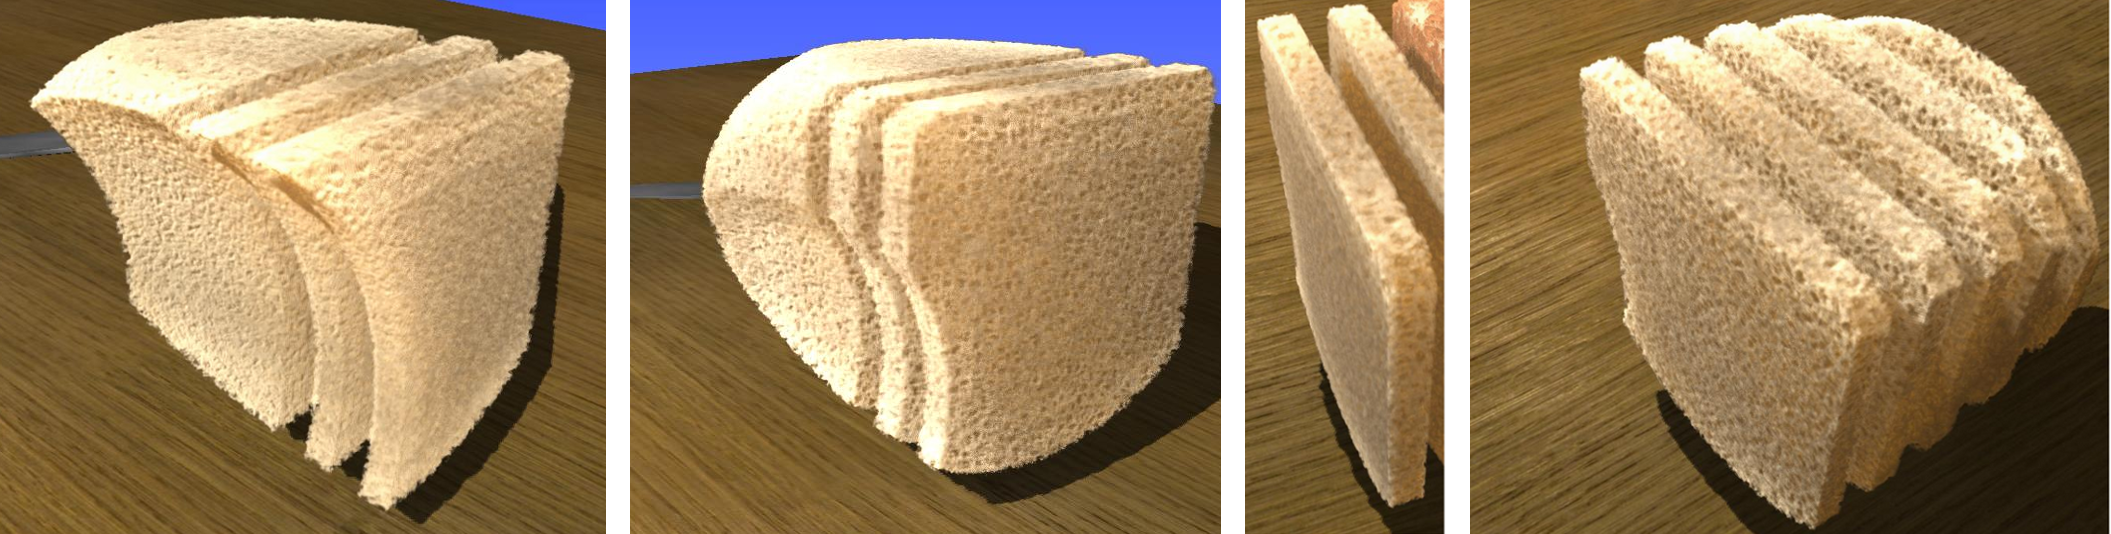
\includegraphics[width=13cm]{figures/crumb}}
  \caption{Miga de pan sintetizada, vista desde distintos ángulos.}
  \label{fg:crumb}
\end{figure}


\begin{figure}
  \centerline{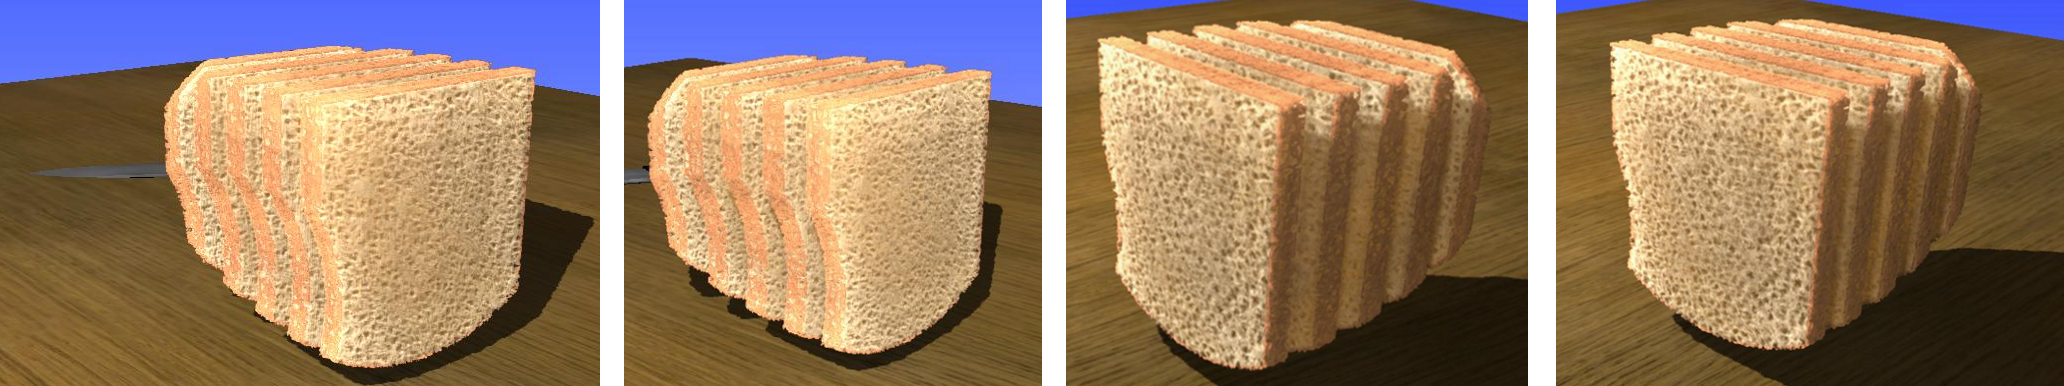
\includegraphics[width=13cm]{figures/results2}}
  \caption{Miga de pan sintetizada, vista desde distintos ángulos (con corteza agregada).}
  \label{fg:results2}
\end{figure}

Si bien es posible la obtención de distintas geometrías de manera sencilla y prácticamente de manera automática, todavía existen limitaciones en cuanto a la flexibilidad de los tipos de pan a producir.
Se depende de un sistema dinámico para producir la forma global de la deformación, pero este sistema es difícil de controlar.
Además, no siempre se adapta de manera sencilla a la forma exterior del material.
Debido a esto, en la siguiente sección presentamos un algoritmo más robusto el cual permite superar estas deficiencias.
El mismo continúa con la idea de la utilización de una definición volumétrica del material, pero el mismo está basado en modelos físicos del proceso de fabricado del pan, extraído directamente de la literatura de ingeniería de los alimentos.

\section{Modelado del Pan desde su Proceso de Fabricación}
Para lograr un modelado realista de la geometría de la miga de pan es necesario comprender su proceso físico de formación.

\begin{figure*}
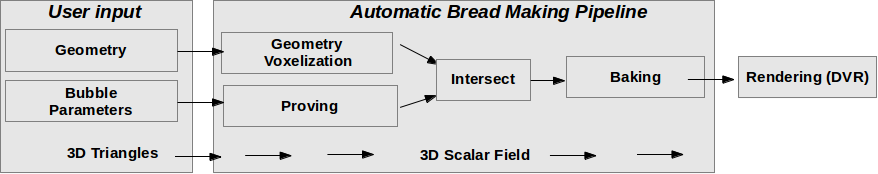
\includegraphics[width=13cm]{figures/pipeline}
\caption{Procedimiento semi-automático para obtener pan sintético foto-realista}
\label{FigPipeline}
\end{figure*}

Utilizando las ideas de la sección anterior, proponemos otro modelo volumétrico de generación de geometrías de migas de pan.
En esta sección proponemos unificar, y diferenciar, los pasos claves presentes en el proceso de fabricación del pan (sobre todo, leudado y cocción).
El procedimiento busca utilizar el proceso físico de generación de geometrías de migas y cortezas de pan a partir de la masa original.
Estos procesos han sido vagamente tenidos en cuenta en la literatura, la cual ha atendido siempre a procesos artísticos más simples, dada la complejidad de los mismos.

En primer lugar, reveeremos el estado del arte del proceso de fabricación del pan.
% e introduciremos modelos matemáticos requeridos para comprender el proceso de cocción.
Luego presentaremos los procesos de modelado, que junto con el modelo de iluminación del siguiente capítulo, permiten obtener imágenes foto realistas de distintos tipos de pan.

\subsection{Trabajo Previo}
El modelado procedimental de geometría reduce fuertemente la necesidad de intervención artística en dominios o situaciones donde la utilización de supervisión repetitiva del proceso se torna impráctica, por ejemplo al modelar ciudades \cite{Parish2001}, planetas \cite{Ebert2002}, edificios \cite{Muller2006}, y plantas \cite{Prusinkiewicz1990}. 
Algunos métodos procedimentales utilizan gramáticas para definir descripciones matemáticas, representando relaciones espaciales entre las primitivas, por ejemplo cubos, cilindros o líneas.
Las estructuras finales usualmente emergen utilizando recursión sobre elementos gramaticales.

Si bien existen algunos ejemplos en la literatura sobre modelado y renderizado de la estructura de migas de pan \cite{Tong2005,Xenakis2007}, los mismos ignoran casi por completo el proceso real de formación.
Algunos trabajos pioneros aplicaron modelos físicos de cocción a determinados tipos de pan para su renderizado, buscando obtener animaciones ({\em e.g.} \cite{Rodriguez-Arenas2011}), pero el modelado de la geometría de las burbujas de la miga del pan no fue tenido en cuenta.

Por otro lado, el modelado procedimental de panes es un tópico multidisciplinario de investigación.
La ingeniería de los alimentos lleva varias décadas de publicaciones en el área, tratando de desarrollar un mejor entendimiento del proceso de formación del pan.
Esta rama de la ciencia muestra que el leudado determina fuertemente las características presentes en la miga de pan, particularmente las burbujas \cite{Babin2006}.
La interacción entre la levadura y algunos nutrientes presentes en la masa produce {\em $CO_{2}$}. 
El radio de las burbujas y sus distribuciones espaciales muestran estructuras con características fractales, exhibiendo autosimilaridad estadística en diferentes escalas de medición.
Determinados trabajos han computado las dimensiones fractales de estas estructuras en determinados tipos de pan \cite{Gonzales2008}, sugiriendo distribuciones fractales uniformes.
El modelado de la cocción del pan es sujeto de numerosos trabajos \cite{Mondal2008}.

El modelado procedimental utilizando fractales también atendió las necesidades de otros variados materiales como montañas \cite{Prusinkiewicz1993}, cráteres lunares, y distribución de las burbujas en quesos \cite{Mandelbrot1982}. 
Adicionalmente, determinados modelos matemáticos complejos representan el comportamiento y el crecimiento de diversos fenómenos naturales.
En computación gráfica, estos modelos son unas de las fundaciones usadas para modelar agua y fluidos \cite{Stam1999,Fedkiw2001}.
Estos trabajos utilizan complejos modelos diferenciales de otras ramas de la ciencia y las aproximan con técnicas numéricas.
En años recientes, la tecnología GPGPU \cite{Owens2007} permitió la posibilidad de alcanzar tiempos reales o interactivos en el cómputo y renderizado de estos modelos numéricos.

A pesar de todos estos avances, el modelado y visualización foto-realista de panes y materiales porosos todavía presenta diversos retos.
Además de un modelo geométrico realista, el renderizado requiere que se represente de manera adecuada los fenómenos de transporte de la luz, incluyendo auto-oclusión, auto-sombreado, transmitancia, translucencia, transparencia, entre otras.
Solamente unas pocas publicaciones proponen atacar ambos problemas, pero utilizando consideraciones artísticas \cite{Xenakis2007}.
Además, estos autores no dan suficientes detalles del modelado y renderización ya que existen derechos de propiedad intelectual, limitando enormemente la reproducción de dichas imágenes.

Por otro lado, la comunidad artística usualmente produce imágenes realistas de pan utilizando fotografías de los mismos, y definiendo geometrías a partir de ellas, junto a la utilización de materiales translúcidos\footnote{http://www.blenderguru.com/tutorials/how-to-create-realistic-bread} y otras consideraciones {\em ad-hoc}\footnote{http://design.tutsplus.com/tutorials/create-a-realistic-loaf-of-bread-in-photoshop--psd-10555}.
Si bien los resultados obtenidos son buenos, los procesos son tediosos y demandan horas.
Además, si se requiere más de una imagen, es necesario repetir todo el proceso desde el principio, lo que torna al mismo muy poco práctico.
Existen numerosas desventajas además de esta.
Por ejemplo, no es posible obtener cortes arbitrarios del material resultante.


\subsection{Visión global del Proceso}
La Fig.~\ref{FigPipeline} muestra el proceso completo de formación de geometrías sintéticas de pan.
Todos los pasos se aplican sobre campos escalares.
Los usuarios pueden proveer el sistema con un modelo de tres dimensiones de su preferencia, o dejar que el sistema provea un pan de forma estándar ({\em croissants}, {\em baguettes}, etc.).
La geometría introducida se voxeliza para proceder a las siguientes etapas.
En la simulación del proceso de leudado, el usuario puede parametrizar la textura del pan (cantidad y tamaño de las burbujas y su distribución), o nuevamente dejar que el sistema provea parámetros estándar que producen tipos de pan conocidos.
La masa cruda será intersectada con la geometría voxelizada para obtener un campo escalar, el cual tiene la forma externa que provee el usuario (o el sistema), con el interior de la misma compuesta de las burbujas procedentes de los parámetros establecidos (ver Sección~\ref{breadprov}).
Luego, se computa un modelo de cocción específico \cite{Powathil2004} para deformar el campo escalar (y las burbujas de éste), de acuerdo a los efectos que produce la cocción en el proceso de formación del pan.
El último paso aplica renderizado directo de volúmenes (direct volume rendering, DVR) \cite{Kruger2003} al campo escalar resultado de la cocción, obteniendo imágenes realistas del pan resultante.

%====================================================================

\subsection{Voxelización de la Geometría}

En nuestro modelo es posible generar panes con geometrías arbitrarias, supliendo un modelo de triángulos en algún formato estándar.
El modelo consta de un conjunto de pasos. El primer paso de la secuencia voxeliza un modelo provisto por un usuario con la utilidad de código abierto {\tt binvox} \footnote{http://www.cs.princeton.edu/~min/binvox/} \cite{Nooruddin2003}.
La voxelización genera un campo escalar binario, con $1$ representando que el voxel dado está dentro de la geometría, y $0$ significando que el voxel está fuera de la geometría.
El paso de leudado (siguiente subsección) genera la textura del material que se ubica dentro de esta geometría voxelizada.
Esto permite generar panes con formas arbitrarias, tales como {\em baguettes}, {\em croissants}, {\em lactal}, u otros menos comunes (una tetera o un conejo).

Un sub-producto importante de la matriz de geometría es un campo escalar secundario que puede ser obtenido por medio de una transformación de distancia.
La transformación de distancia genera una matriz $n$-dimensional con las mismas dimensiones que la matriz que se transforma \cite{osh03}.
La transformación computa, para cada entrada distinta de cero en la matriz, la distancia más cercana a una entrada nula de dicha matriz.
Dada una matríz $n$-dimensional $M$, el algoritmo genera una matriz a valores reales $DF_{M}[i]$ con las mismas dimensiones que $M$,


$$  DF_{M}[i] = \min \bigg\{ \delta(i,j): M[j] = 0 \bigg\},$$

%\begin{align*}
%M'[i] &= min(d(i,j)), M[i] != 0, M[j] = 0\\
%M'[i] &= 0, M[i] = 0,
%\end{align*}

\noindent
donde $\delta(i,j)$ podría ser la distancia de Manhattan o la distancia Euclideana en un espacio $n$ dimensional.
Las entradas de la matriz lejanas a los bordes del objeto tomar valores más altos que aquellas cercanas a los mismos.
De esta manera se obtiene un mapa de la distancia de cada voxel a las superficies tridimensionales del objeto.
Este campo escalar de distancias será requerido en etapas posteriores del proceso.


\subsection{Simulación del Leudado}
\label{breadprov}
Como fue establecido, la textura observable en la masa cruda del pan está compuesta de burbujas, cuya distribución exacta es el resultado de procesos complejos, entre ellos, reacciones químicas, y deformaciones físicas de la masa.
El paso de leudado consta en primera instancia del crecimiento libre de las burbujas, producido por seres vivos, la levadura.
Luego, el cocinero interviene la masa deformándola de diversas maneras.
Finalmente el paso de cocción produce la textura y distribución de burbujas finales.
Los estudios fenomenológicos de estas texturas utilizan tomografía de rayos X y extracción de características sobre las mismas \cite{Gonzales2008,Babin2006,VanDyck2014}.
Buscando obtener una variabilidad similar, en esta tesis generamos distribuciones de burbujas con un modelo basado en fractales, inspirado en las distribuciones de burbujas presentes en el queso, y la textura inducida por los cráteres lunares, propuesto en \cite{Mandelbrot1982}.
Luego validamos los mismos utilizando el método multifractal denominado {\em Sandbox} (caja de arena, ya que realiza cálculos sobre una distribución de puntos aleatoria en la geometría).
Esto será explicado en profundidad en el capítulo de validación.

La textura de la masa es creada procedimentalmente en un campo escalar separado, definido en una matriz de tres dimensiones, de una manera similar a la matriz de geometría en la Subsección arriba.
Cada voxel es iniciado a $1$ (significando que el material aún no tiene burbujas).
El proceso comienza substrayendo esferas de radio $r_{min}$ posicionadas arbitrariamente en el campo escalar (esto se logra seteando a $0$ las celdas respectivas).
Luego, substraemos esferas de radio mayor, nuevamente en posiciones arbitrarias, hasta un radio máximo $r_{max}$.
La relación entre el número de esferas $N_{s}$ a ser sustraídas en cada paso, y sus respectivos radios $r$, está dada por la ley fractal,


\begin{equation*}
N_{s} = \frac{k}{r^{d}},
\end{equation*}

donde $d$ es el exponente fractal que modela la ocurrencia de esferas en relación con su radio, y $k$ controla la cantidad de esferas para cada radio.
Con estos simples parámetros basta para modelar una gran cantidad de texturas en general, particularmente pan.

La Fig.~\ref{FigProving} muestra un ejemplo de un corte en dos dimensiones de este modelo.
Si bien las burbujas esféricas resultantes no son completamente realísticas debido a su forma, los resultados muestran un notorio parecido en tamaños y distribución de tamaños con binarizaciones de cortes reales de masas leudadas (ver \cite{Babin2006}).
Durante la cocción, el campo escalar resultante será sometido a deformaciones geométricas. Consecuentemente, la textura final se ajustará aún más a burbujas de panes reales.
Finalmente, en la sección de validación se buscarán parámetros de generación que ajusten diferentes panes reales. 

\begin{figure}
\center
\includegraphics[width=7cm]{figures/bubbles}
\caption{Simulación Fractal del Leudado de Pan.}
\label{FigProving}
\end{figure}

Luego de la voxelización y la simulación de leudado, las burbujas deben estar presentes sólo en el interior de la geometría.
Para esto, intersectamos ambos campos escalares utilizando un simple producto punto a punto, es decir, una máscara,

\begin{equation*}
P_{2} = P_{1} * G,
\end{equation*}
%
donde $P_{1}$ es el campo $3D$ (matriz) que contiene las burbujas del leudado, y $G$ es el campo escalar que representa a la geometría voxelizada.

La Fig.~\ref{fg:intersectProblem} muestra una versión renderizada de esta intersección.

\begin{figure*}
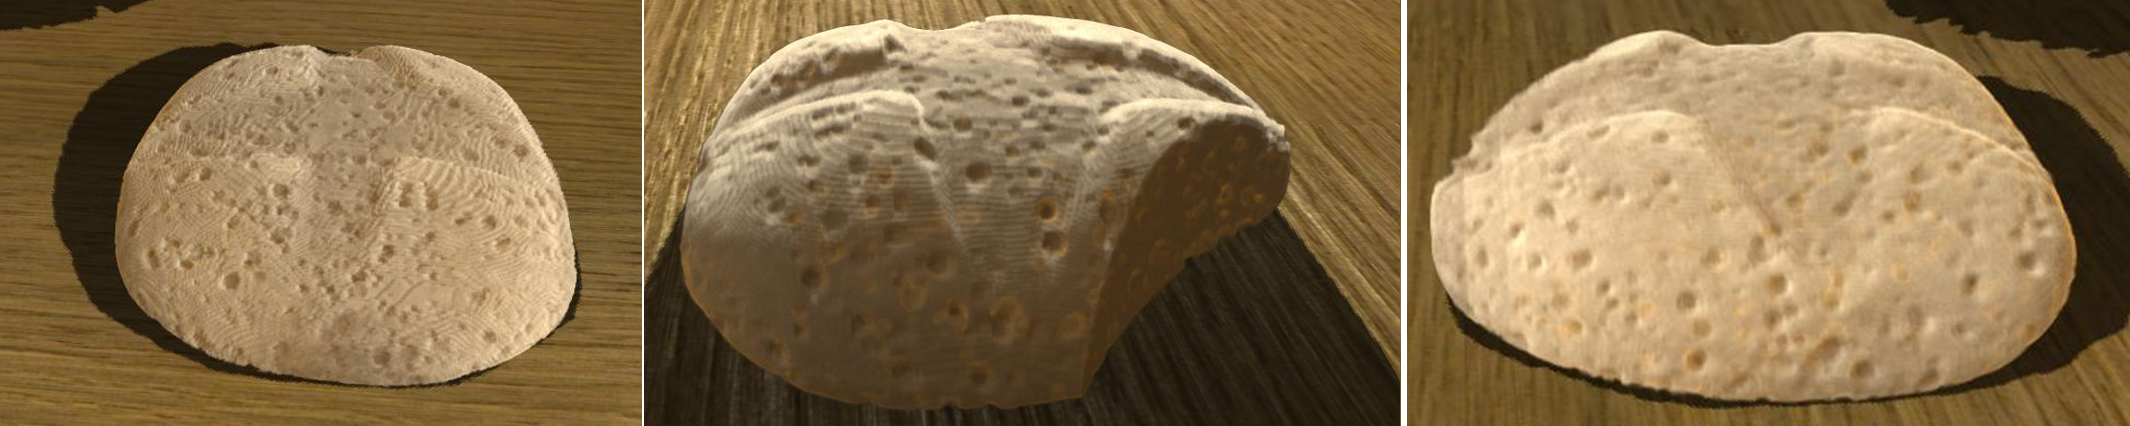
\includegraphics[width=13cm]{figures/intersectProblem}
\caption{Intersección simple de la geometría y de las burbujas provenientes del leudado. A diferencia de masas reales, pueden verse burbujas en la superficie de la masa.}
\label{fg:intersectProblem}
\end{figure*}

Si bien los resultados pueden parecer realistas, en panes reales, no es habitual que las burbujas sean visibles en la superficie, debido al leudado y cocción reales.
Para solucionar este problema, utilizamos el campo escalar de distancias que computamos previamente, para deshabilitar la generación de burbujas en zonas cercanas a los bordes de la geometría, de acuerdo a cierto valor umbral, el cual será un parámetro.
El campo escalar binario resultante se computa de la siguiente manera,

%\begin{align*}
%DF    &= distField(G),\\
%interior &= DF > umbral,\\
%masa &= G - interior*(1-P_{2}),
%\end{align*}
%
%donde $DF$ es el campo escalar de distancias a la superficie, computado a partir de la geometría de entrada, voxelizada, y $umbral$ es un parámetro que determina el ancho de la región exterior, donde no pueden crearse burbujas.
%Computamos la masa final substrayendo las burbujas ($1-P_{2}$) de la geometría original, pero limitada a la región {\em interior} que acabamos de definir.
Las Figs.~\ref{fg:proving} y \ref{fg:provingBunny} muestran resultados de limitar las interacciones de burbujas a la región interior de la geometría original, donde se observa que no existen burbujas en la superficie de la masa, como ocurre en masas reales.
Las imágenes muestran que el método definido es capaz de producir imágenes realistas de panes crudos con formas arbitrarias.
Cabe remarcar que el modelo es lo suficientemente flexible, permitiendo renderizar el material en cualquier etapa de su proceso de fabricación, además de poder realizar cortes arbitrarios del mismo.

\begin{figure*}
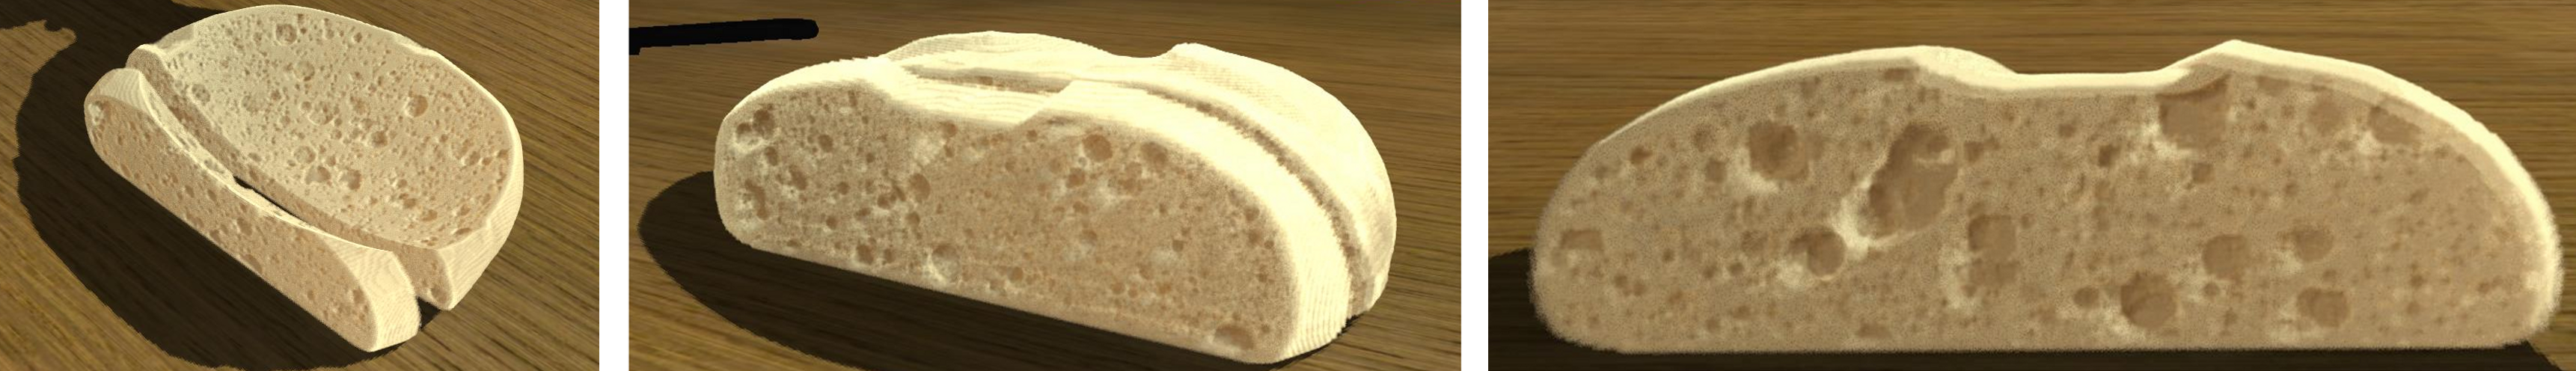
\includegraphics[width=13cm]{figures/prebakebread}
\caption{Pan luego del leudado, y antes de la cocción.}
\label{fg:proving}
\end{figure*}

\begin{figure*}
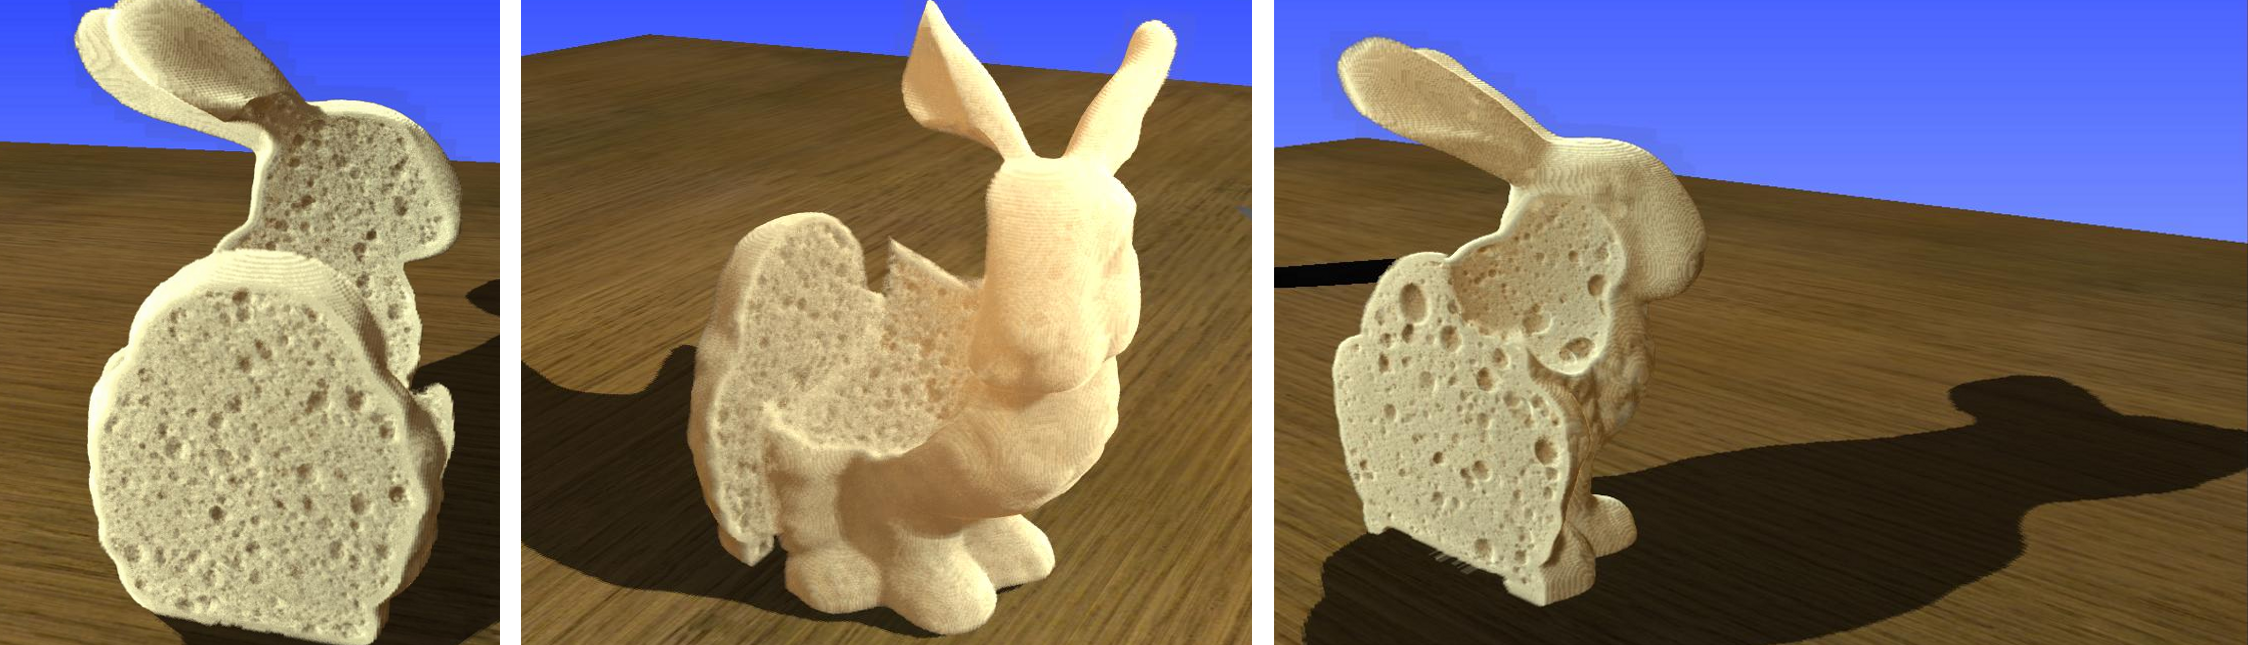
\includegraphics[width=13cm]{figures/prebakebunny}
\caption{Conejo de pan, luego del leudado, y antes de la cocción.}
\label{fg:provingBunny}
\end{figure*}

%====================================================================
\subsection{Cocción}
%To adequately simulate the bread baking process, mathematical models should be able to accurately model the heat and mass transfer in dough.
Los modelos matemáticos del proceso de cocción del pan deben ser capaces de modelar correctamente las transferencias de calor y masa en el mismo.
Los modelos físicos más completos del proceso producen soluciones precisas a la distribución de temperaturas en la masa durante la cocción.
Sin embargo, estos modelos son usualmente muy complejos para implementar y son muy costosos computacionalmente.
Además, sólo los modelos más complejos toman en consideración la formación de la corteza del pan.
La corteza, por otro lado, aún carece de una definición formal~\cite{Vanin2009}.
Por lo tanto, los modelos antes citados incluyen sólo una simplificación de la formación de la misma, muy lejos de lo que ocurre en la cocción real.

Los resultados más relevantes en la literatura sugieren que un modelo unidimensional de la cocción puede ser suficiente para la mayoría de los casos prácticos.
Por ejemplo, Purlis~\cite{Purlis2011} modela la cocción del pan como un problema unidimensional, representando la geometría como un cilindro infinito.
Otros trabajos asumen sólo una coordenada radial, resultando también en modelos $1D$~\cite{Powathil2004, Thorvaldsson1999}.
Estos trabajos muestran que utilizar una representación de una única dimensión produce resultados casi idénticos a aquellos que se obtienen utilizando un mayor número de dimensiones, ya que el efecto de la cocción en las burbujas es la menos importante en el proceso de fabricación del pan.

La simulación numérica que implementamos está basada en el esquema de diferencias finitas propuesto por Powathil~\cite{Powathil2004}, y Thorvaldsson y Janestead~\cite{Thorvaldsson1999}. 
El sistema presentado consiste de un conjunto de tres ecuaciones acopladas que describen transferencia de calor, difusión de varpor de agua y difusión de agua líquida.
En nuestro algoritmo, sólo utilizamos las temperaturas ($T$) como entrada para las siguientes etapas de la formación del pan.
La Ec.~\ref{Eq:heat} modela transferencia de calor en la masa del pan, tomando en consideración el balance de energía y evaporación del agua debido a la temperatura~\cite{Thorvaldsson1999},
%
\begin{equation}
\label{Eq:heat}
\frac{\partial T}{\partial t} = \frac{1}{\rho C_{p}} \frac{\partial}{\partial x} \left ( k \frac{\partial T}{\partial x} \right ) + \frac{\lambda}{C_{p}} \frac{\partial W}{\partial t}+\frac{\lambda W}{ \rho C_{p} }\frac{\partial \rho}{\partial t},
\end{equation}
%
donde $T$ es la temperatura, $x$ es la coordenada radial, $t$ es el tiempo, $C_{p}$ el calor específico, $\rho$ la densidad, $k$ la conductividad térmica, $\lambda$ es el calor latente de la evaporación de agua, y $W(x,t)$ es el contenido de agua líquida. 
Las condiciones iniciales
%
\begin{align*}
T(x,0) &= T_{0}(x), 0\le x \le L/2,
\end{align*}
y las condiciones de borde (continuidad y suavidad) definen el modelo,
\begin{align*}
\left ( \frac{\partial T}{\partial x} \right )_{x=L/2} &= 0 , t > 0 \\
-k \left ( \frac{\partial T}{\partial x} \right )_{x=0} &= h_{r}(T_{r}-T_{s}) + h_{c}(T_{air}-T_{s}) - \lambda \rho D_{w} \left (\frac{\partial W}{\partial x} \right )_{x=0}
\end{align*}
%
donde $h_{r}$ y $h_{c}$ son subtérminos del coeficiente de transferencia de calor ($h = h_{r}+h_{c}$), $T_{air}$, $T_{s}$, $T_{r}$ son temperaturas en el aire circundante, en la superficie del pan, y en la fuente de radiación, respectivamente, $L$ es el alto del pan($x = L/2$ es el centro del pan y $x = 0$ es el contorno del mismo), $D_{w}$ representa la difusividad del agua líquida, y $T_{0}$ la temperatura inicial. 
Las temperaturas están expresadas en Kelvin ($K$). 
El modelo consta de ecuaciones similares para la difusión del vapor de agua ($W$) y difusión de agua líquida ($V$).
Otros detalles del modelo pueden ser consultados en \cite{Thorvaldsson1999}.
En nuestro trabajo, utilizamos este modelo para obtener un mapa de temperaturas al final del proceso de cocción.
Estas temperaturas afectarán posteriormente las formas y tamaños de las burbujas.

La simulación de la cocción define el horno a una temperatura típica (por defecto utilizamos $210^{\circ}C$) y discretiza el tiempo en intervalos $\Delta t = 30s$.
De la simulación se obtiene un arreglo $Temp$, de tamaño $N_{grid}$, compuesto por valores de temperatura.
Por estabilidad numérica, utilizamos $N_{grid}=32$ (como en el trabajo original) e interpolamos las temperaturas para obtener mayores resoluciones ($N_{int}$). 
%Each value represents a dough position after $M$ baking time steps. 

El vector obtenido presenta temperaturas decrecientes de $R = 0$ a $R = L/2$, ya que el centro y el borde del pan poseen la menor y la mayor temperatura, respectivamente, luego de la cocción (el calor fluye desde la corteza hacia el centro del pan). 
Si utilizamos el campo escalar de distancias computado previamente, en conjunto con el vector de temperaturas, podemos mapear distancias a temperaturas.
Esto permite definir temperaturas en el campo escalar de forma compatible a una simulación $3D$.
Basados en estos razonamientos, mapeamos el vector de temperaturas $Temp$ en $3D$ de la siguiente manera,

\begin{equation*}
\displaystyle R(x,y,z) = Temp[ round( DF(x,y,z) ) ], 
\end{equation*}
%
donde $R$ es el campo escalar resultante del mapeo, y $x$, $y$ y $z$ son coordenadas $3D$ en $R$. Cuando $DF(x,y,z) = 0$, la posición actual $3D$ se encuentra en la superficie de la geometría, y $Temp[0]$ se mapea $R(x,y,z)$.
Cuando $DF(x,y,z) > 0$, mapeamos una temperatura menor a $R$, ya que la posición actual se encuentra en el interior de la geometría.
La Fig.~\ref{fg:baking} muestra cortes del resultado de este mapeo ($R$), usando temperaturas resultantes de un tiempo arbitrario de cocción, en los tres planos Cartesianos. 
Las imágenes son casi idénticas a lo que se obtendría con una simulación $3D$~\cite{Purlis2010}.

\begin{figure*}
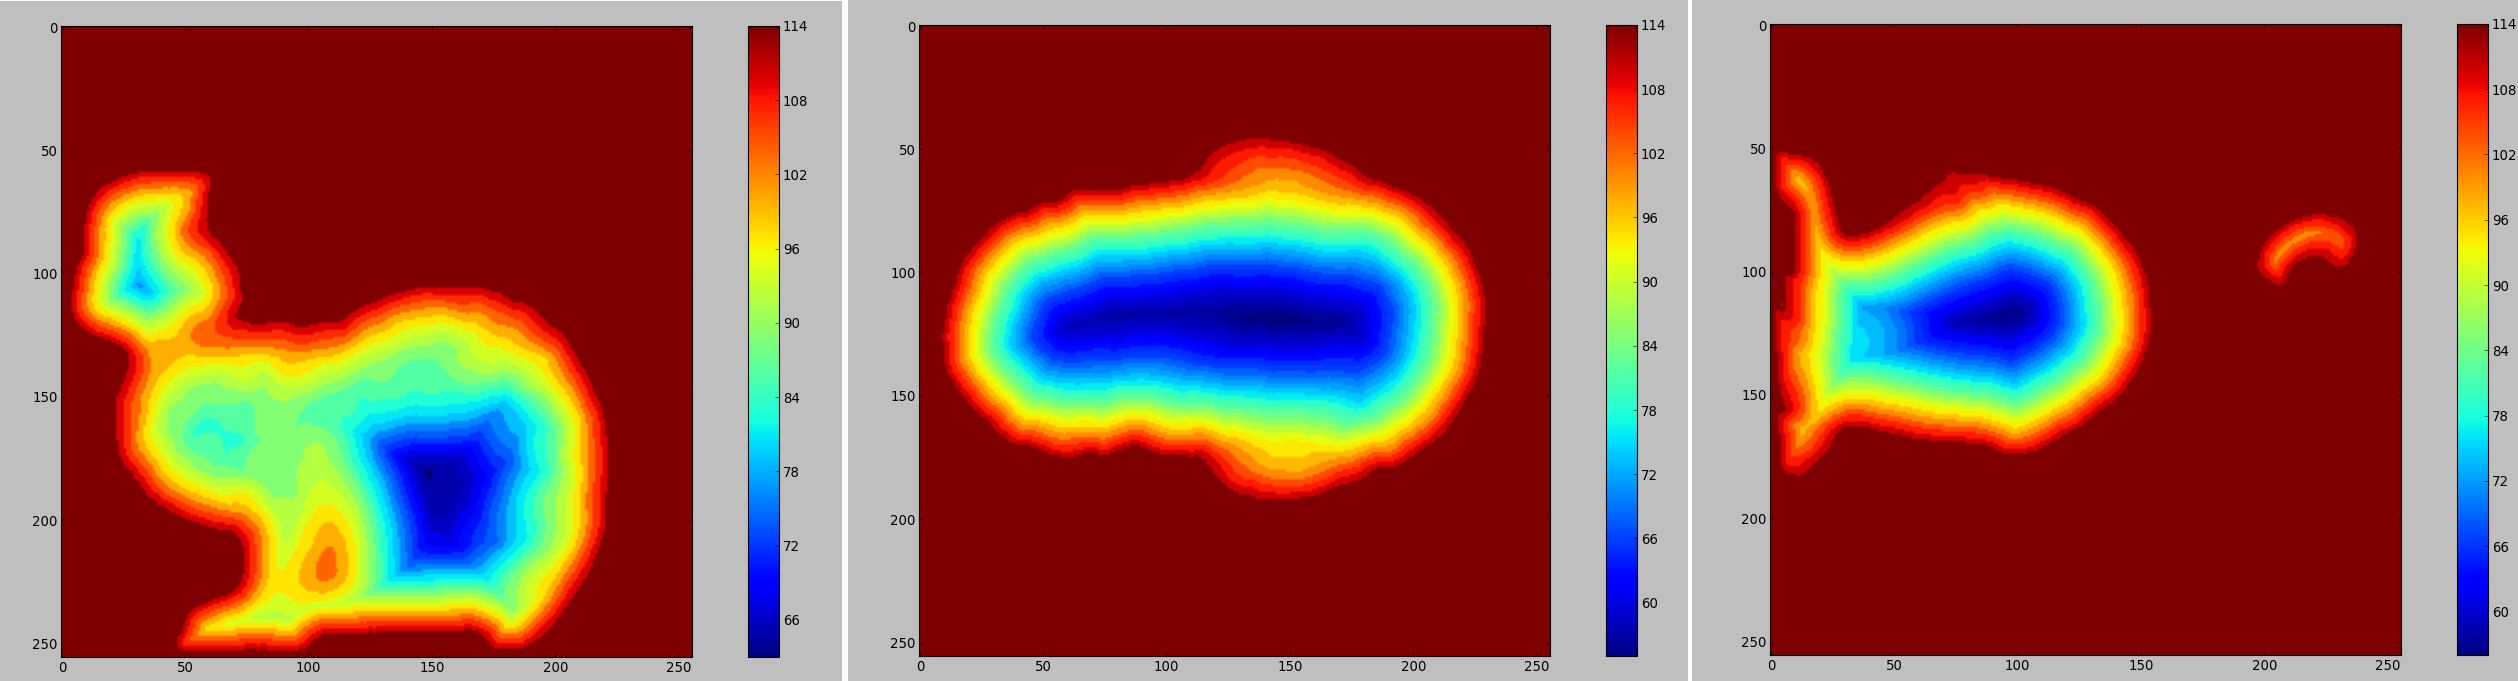
\includegraphics[width=13cm]{figures/tempsbunny}
\caption{Temperaturas unidimensionales mapeadas a un campo escalar con forma de conejo. Las imágenes muestran que la distribución de temperaturas es similar a una simulación en tres dimensiones.}
\label{fg:baking}
\end{figure*}

Luego de cierto número de pasos de simulación ($t=20$ en nuestro caso), computamos el campo vectorial del gradiente ($g$) de $R$ \cite{Gonzalez2006}, y luego suavizamos el mismo utilizando un kernel Gaussiano.
Finalmente, utilizamos las versiones suavizadas para deformar el campo escalar de la siguiente manera,

\begin{align*}
\displaystyle
u &= x+p*g'_{x}[x,y,z],\\
v &= y+p*g'_{y}[x,y,z],\\
w &= z+p*g'_{z}[x,y,z]
\end{align*}
donde $(u,v,w)$ son las coordenadas en el campo escalar resultante, ($x,y,z$) son las coordenadas originales, $p$ es un parámetro real positivo que denota la intensidad con la que se deforma el campo (controla el efecto neto de la cocción en las burbujas), y las $g'$s son las versiones suavizadas del gradiente original $g$.
%Fig.~\ref{FigBakingVectorField} also shows the computed gradient, where using $[-g_{x},-g_{y}]$ produces a similar vector but in the clockwise direction that can be applied with similar effects on the bubbles. 
La Fig.~\ref{fg:bakedbubbles} muestra cortes $2D$ de campos escalares luego de aplicado el proceso de cocción a diferentes formas.

\begin{figure*}
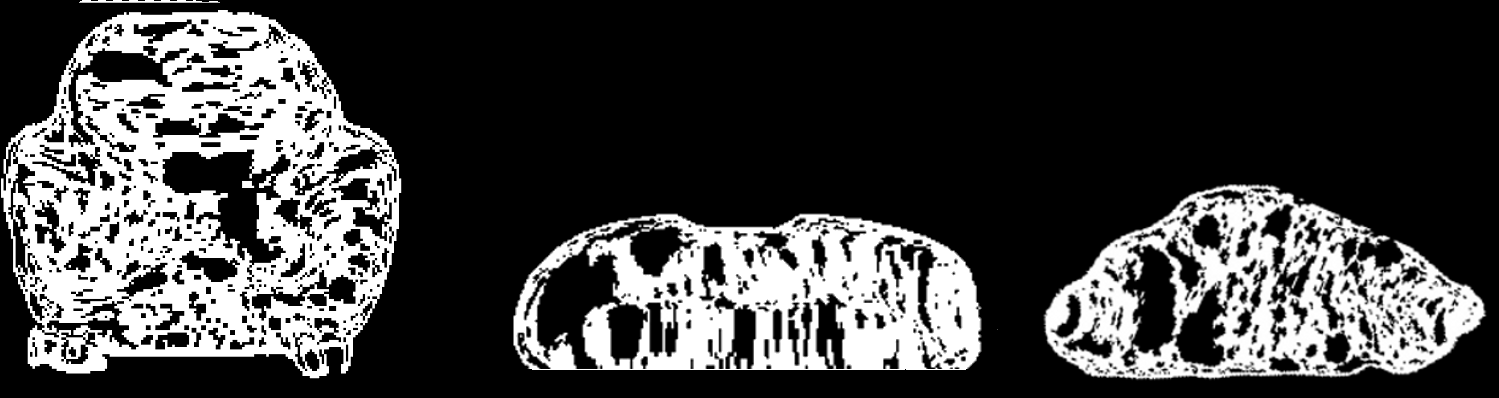
\includegraphics[width=13cm]{figures/bakedbubbles}
\caption{Cortes bidimensionales con burbujas deformadas por el proceso de cocción en diferentes tipos de panes.}
\label{fg:bakedbubbles}
\end{figure*}

El parámetro $p$ puede ser utilizado para sintetizar diferentes apariencias de miga de pan, desde cruda hasta burbujas con mucha deformación (ver Fig.~\ref{fg:parameterp}).
Cuando incrementamos $p$, forzamos a las burbujas a seguir más ajustadamente la forma exterior del pan. 
La imagen también muestra que el método deforma más pronunciadamente las burbujas más cercanas a la corteza.

\begin{figure*}
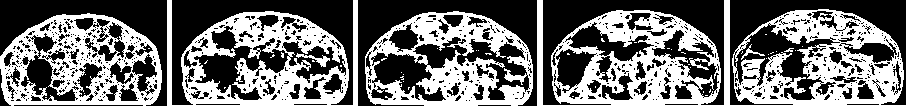
\includegraphics[width=13cm]{figures/parameterp}
\caption{Efecto del parámetro $p$: de izquierda a derecha $p$ es $0$, $5$, $10$,$15$, y $25$, respectivamente.}
\label{fg:parameterp}
\end{figure*}


\subsection{Formación de la Corteza}
El modelo de cocción que hemos introducido no incluye detalles precisos de la formación de la corteza.
En estas ecuaciones, la corteza se asume es producida en la superficie del material, a determinada temperatura, pero esta simplificación está lejana a lo que ocurre actualmente en el proceso real de cocción.
La literatura de ingeniería de los alimentos define la corteza como una interfase que emerge entre la masa y el aire.
Entre sus principales características se encuentra la formación de un material más denso en la superficie, y una diferenciación de color.
Sin embargo, los detalles precisos acerca de cómo esto ocurre se desconocen, por lo tanto, la apariencia exacta de la misma, está lejos de ser comprendida en los modelos presentes acutalmente.

Debido a esto, y basados en la aproximación inicial asumida, utilizamos el campo escalar de distancias computado previamente para definir una región de corteza.
Esta elección está fundada en el hecho de que la corteza está mayormente determinada por un frente de evaporación que resulta de la temperatura \cite{Jefferson2007}.
En otras palabras, obtenemos las posiciones utilizando el campo escalar mencionado, ya que hemos definido una relación entre la temperatura y la distancia a la superficie.
Además, obtenemos diferentes apariencias de pan utilizando un parámetro de distancia que determina diferentes anchos de corteza.
\subsection{Tiempos de cómputo}
En la implementación utilizamos Python\footnote{python.org} y Cython\footnote{cython.org}.
En la Tabla~\ref{tab:computingtimes} se muestran tiempos de cómputo típicos para los distintos pasos en la simulación de la formación del pan, detallados en secciones anteriores. %In addition, rendering times with DVR are in the order of $~300$ ms (milliseconds), achieving interactive framerates.

\begin{table}[h!]
       % Give a unique label
% For LaTeX tables use
\begin{tabular}{lllll}
\hline\noalign{\smallskip}
Resolución del Campo Escalar & $256^{3}$ & $384^{3}$  & $512^{3}$ \\
\noalign{\smallskip}\hline\noalign{\smallskip}
Leudado & 0.28 & 0.97 & 2.29 \\
Intersección & 8 & 10.81 & 14.97 \\
Campo escalar de Distancias & 7 & 23.73 & 56 \\
Cocción & 19.92 & 51.15 & 117.27 \\
%Rendering & 1s & 4s & 0\% \\
\noalign{\smallskip}\hline
\end{tabular}
\caption{Tiempos de cómputo típicos en nuestro modelo expresados en segundos.}
\label{tab:computingtimes}
\end{table}

Es importante mencionar que la mayor parte del tiempo de cómputo en la cocción está dedicado al cómputo del gradiente, y no al proceso de cocción en sí.
Debido a los costos computacionales en resoluciones superiores, el usuario puede generar vistas previas de los panes utilizando campos escalares con menores resoluciones.


\section{Resultados}
En esta sección presentamos imágenes renderizadas de geometrías de pan obtenidas utilizando nuestro modelo.

Las Figs.~\ref{fg:renders}, \ref{fg:renders2}, y ~\ref{fg:renders3} muestran imágenes renderizadas de panes obtenidos en este trabajo.
Las Figs.~\ref{fg:renders} y ~\ref{fg:renders2} marcan las diferencias en realismo entre resoluciones del campo escalar de ($256^{3}$) y  ($512^{3}$) respectivamente.
La Fig.~\ref{fg:renders3} muestra versiones de alta resolución en el campo escalar de otras geometrías, incluyendo panes con formas de conejos.
La Fig.~\ref{fg:croissant} muestra un pan con forma de {\em croissant} en el cual se han hechos distintos cortes, los cuales demuestran que el método permite obtener imágenes de partes arbitrarias del material.
Las Figs.~\ref{fg:bigalveoli} y ~\ref{fg:bakedbunny} muestran un pan típico y uno con forma de conejo, mostrando burbujas grandes y las burbujas deformadas como resultado del proceso de cocción.
Además se cambió el color de la miga.

Los colores de corteza y miga son parámetros definibles por el usuario. Los cortes en la miga son fácilmente producidos cambiando a $0$ las regiones deseadas en el campo escalar luego de la cocción, y antes del renderizado.

\begin{figure*}[!ht]
\begin{center}
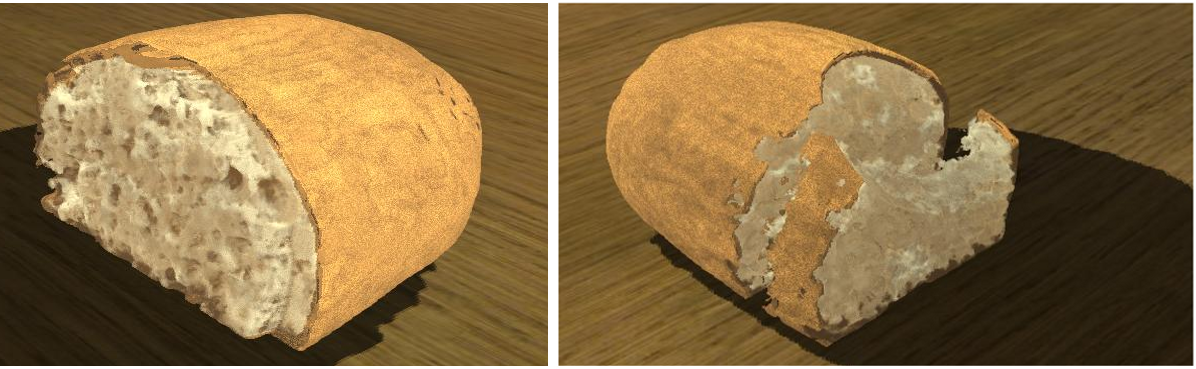
\includegraphics[width=13cm]{figures/otherbread}
\caption{Cortes de pan luego de la cocción, utilizando un campo escalar de dimensiones $256^{3}$. Las imágenes muestran que la miga y la corteza son consideradas en nuestro modelo.}
\label{fg:renders}
\end{center}
\end{figure*}

\begin{figure*}[!ht]
\begin{center}
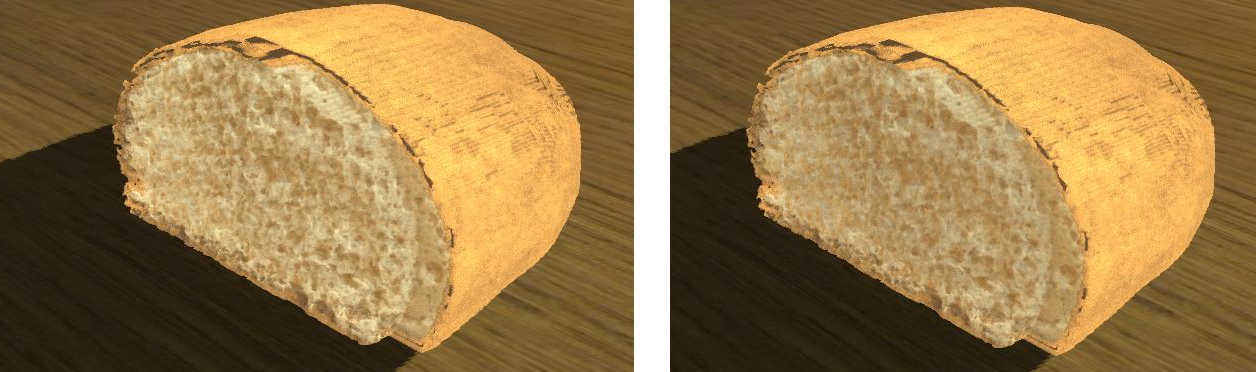
\includegraphics[width=13cm]{figures/otherbread512}
\caption{Cortes de pan luego de la cocción, utilizando un campo escalar de dimensiones $512^{3}$. Se observan mayores detalles en la miga, lo cual aumenta el realismo de la imagen.}
\label{fg:renders2}
\end{center}
\end{figure*}

\begin{figure*}[!ht]
\begin{center}
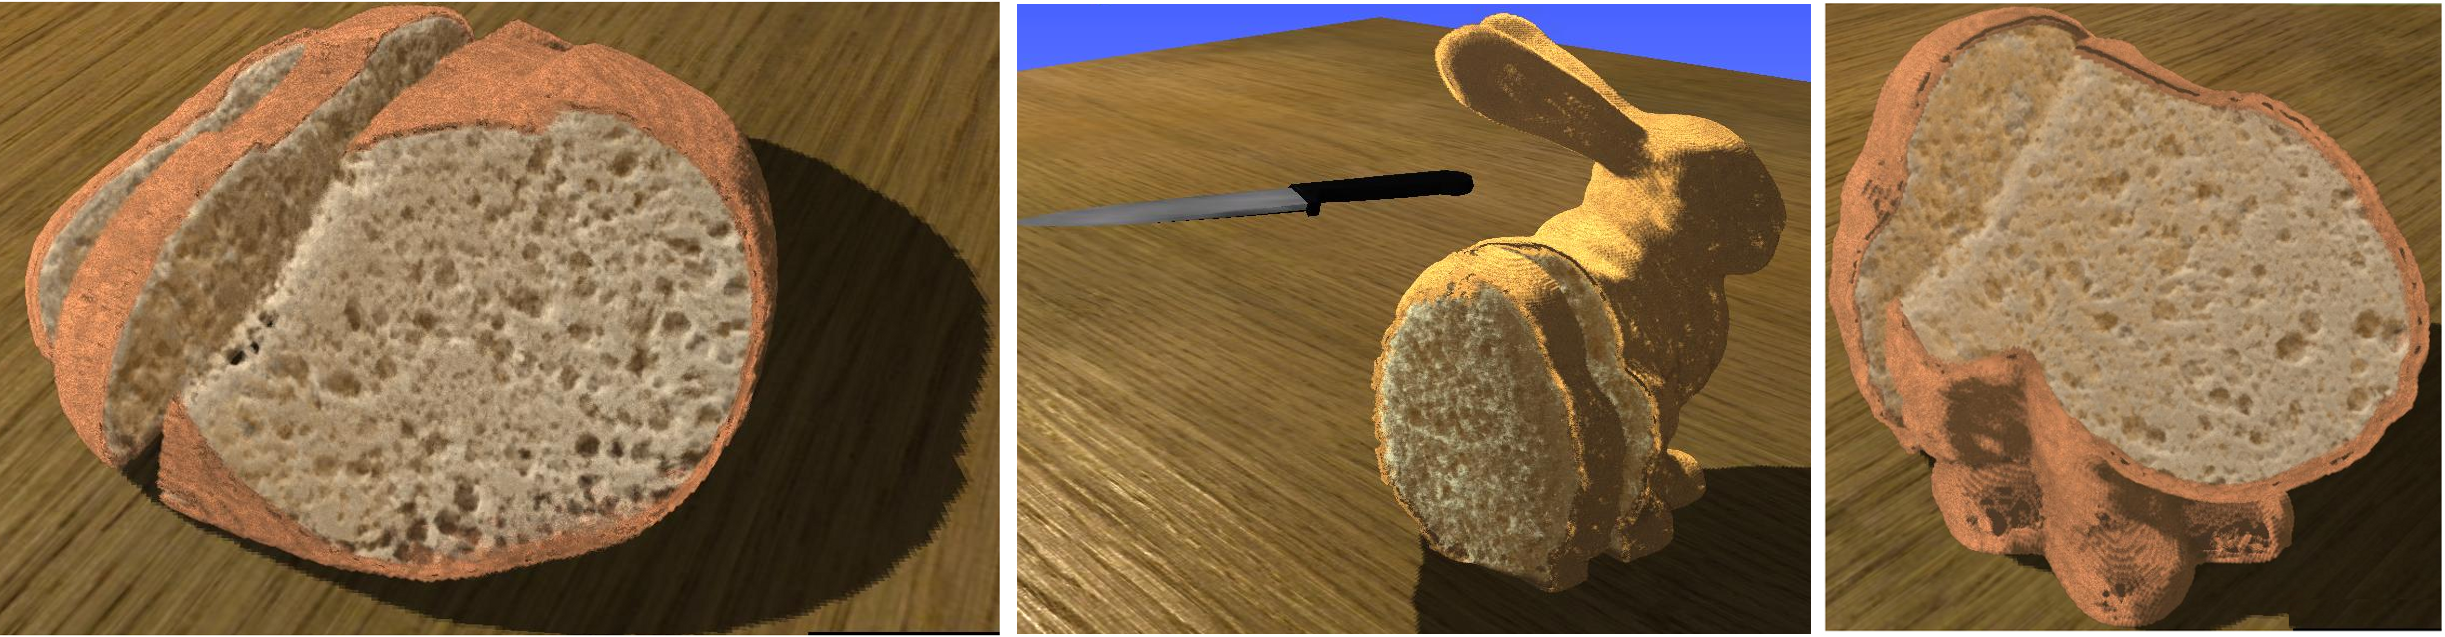
\includegraphics[width=13cm]{figures/final}
\caption{Cortes de pan luego de la cocción con distintas geometrías.}
\label{fg:renders3}
\end{center}
\end{figure*}

\begin{figure*}[!ht]
\begin{center}
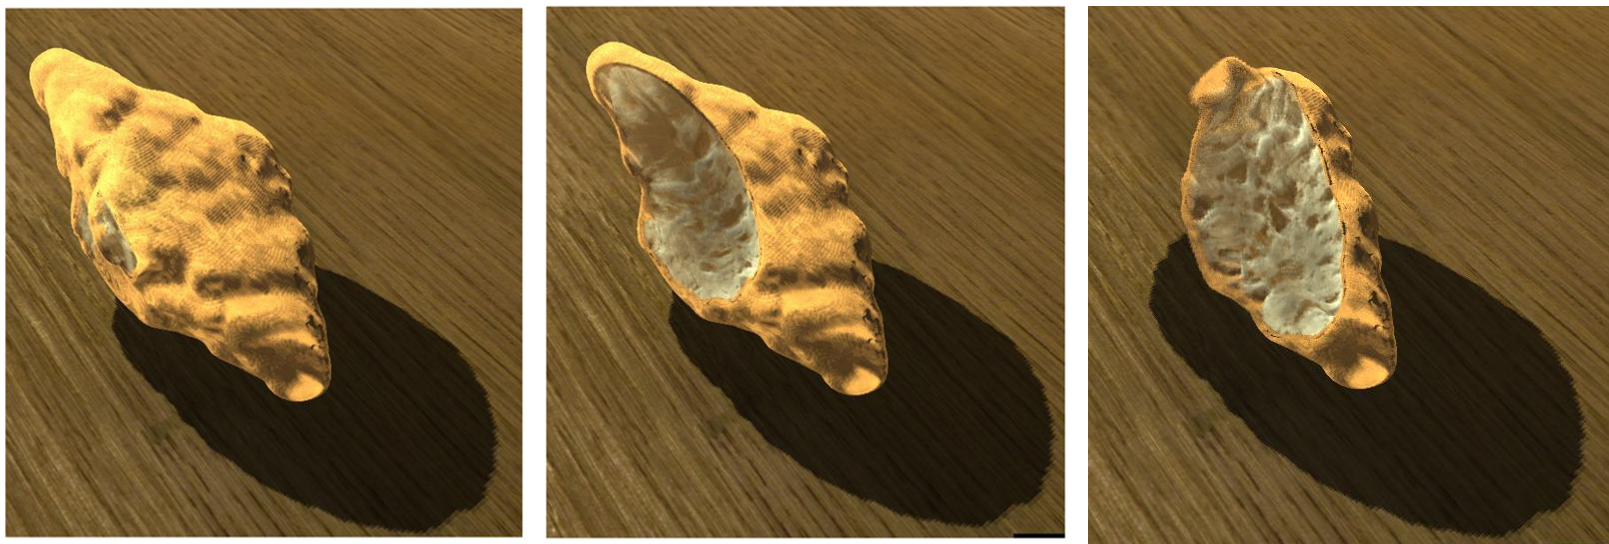
\includegraphics[width=13cm]{figures/croissant}
\caption{Cortes de una Croissant luego de la cocción. La imagen muestra el interior de la miga en distintas regiones del volumen.}
\label{fg:croissant}
\end{center}
\end{figure*}

\begin{figure*}[!ht]
\begin{center}
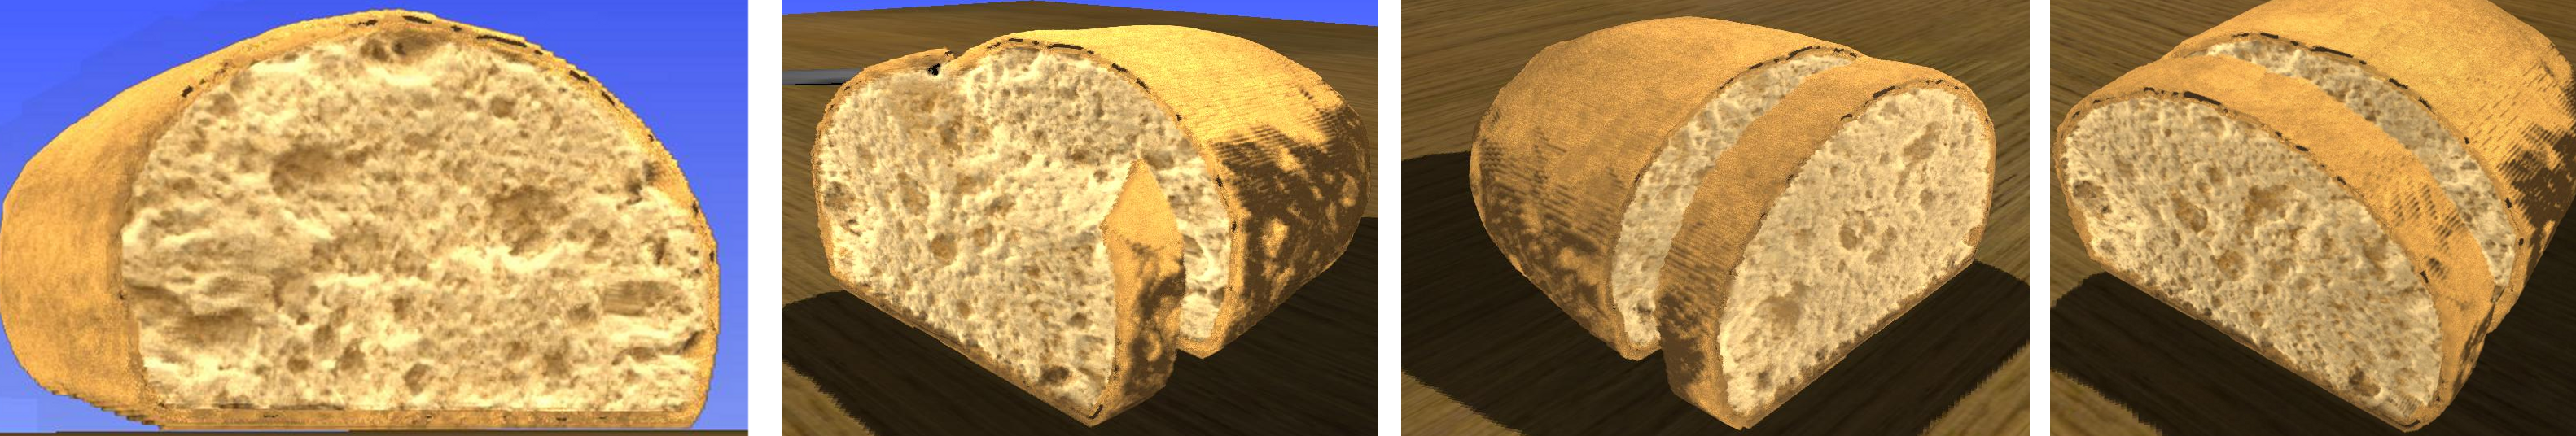
\includegraphics[width=13cm]{figures/baked}
\caption{Cortes de pan luego de la cocción, con burbujas de mayor tamaño, como es típico en determinados panes reales.}
\label{fg:bigalveoli}
\end{center}
\end{figure*}

\begin{figure*}[!ht]
\begin{center}
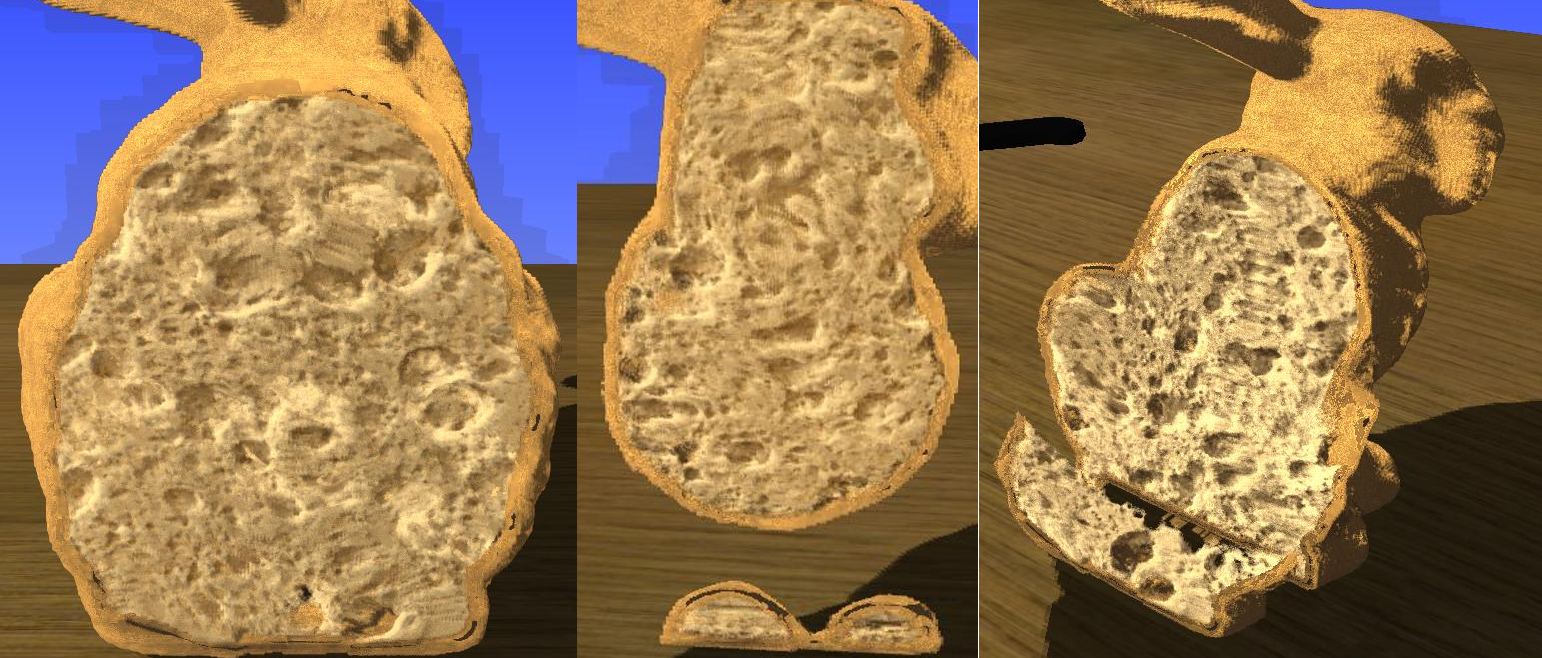
\includegraphics[width=13cm]{figures/bakedbunny}
\caption{Cortes de pan luego de la cocción con burbujas de mayor tamaño. Además, puede observarse más claramente el efecto de la cocción en la deformación de las burbujas, las cuales tienden a seguir la forma de la corteza.}
\label{fg:bakedbunny}
\end{center}
\end{figure*}

%Images show realistic bread appearances, suitable for photo-realistic rendering and serious ga\-mes \cite{Susi2007}. 


%This is illustrated in Figure~, where arrow lengths indicate vector modulus. The image shows that the field's influence is higher near the crust, mostly deforming outer bubbles. This behavior is consistent with real bread crumbs: baking influences the outer bubbles' shape, elongating them parallel to the crust \cite{Scanlon2001}, in other words, following its isotherms.


%\subsection{Leudado}
%El leudado es el principal responsable de la apariencia visual de las burbujas en la miga de pan \cite{}.

%Los patrones observados en la distribución de las burbujas son resultado de procesos complejos, entre los que encontramos reacciones químicas y deformaciones físicas. Este paso en la fabricación consiste en un crecimiento libre de las burbujas, producido por organismos vivos (levadura) en la masa sin cocción del pan.

%Diferentes estudios fenomenológicos de la distribución de burbujas aparecen en la literatura. Los mismos utilizan tomografía de rayos X y extracción de características sobre imágenes para obtener una imagen y modelar las mismas \cite{Babin2006,Gonzales2008,VanDyck2014}.

%El modelo utilizado está inspirado en un modelo propuesto en \cite{Mandelbrot1982}, el cual intenta modelar quesos y distribuciones de cráteres en cuerpos celestes. Validaremos la distribución obtenida utilizando una métrica multi-fractal basada en el espectro multifractal Sandbox.

%Se comienza con una esfera de radio $v = 1$ voxels. Este radio es incrementado en cada iteración. En cada paso, se extraen un número de esferas proporcional al radio:


%\begin{equation}
%N_{esferas} = \frac{k}{r^{d}},
%\end{equation}

%\noindent donde $k$ y $d$ son parámetros con valores reales, y $r$ es el radio de la esfera.

%La Figura~\ref{FigProving} muestra un ejemplo en dos dimensiones de este proceso, donde $d$ controla la relación existente entre los radios de las esferas y $k$ el número de esferas que extraemos en cada paso.

%Las imágenes muestran una apariencia similar a las que pueden observarse en diferentes espumas (café, jabón, cerveza), y en particular a la que muestra el leudado del pan \cite{Babin2006}. 

%\begin{figure}
%\includegraphics[scale=0.28]{bubbles.png}
%\caption{Fractal bread proving simulation.}
%\label{FigProving}
%\end{figure}

%En la sección de validación ajustaremos los parámetros para adecuarlos a los de imágenes de migas reales de pan.

%\subsection{Cocción}
%\subsubsection{Modelo Matemático}

%El modelo matemático del proceso de cocción simula la transferencia de calor y masa en diversos alimentos, entre ellos el pan.  En esta tesis utilizaremos modelos de una dimensión~\cite{Thorvaldsson1999,Purlis2010}. Por ejemplo, Purlis~\cite{Purlis2010} modela la geometría del pan como un cilindro infinito.

%Utilizaremos la solución numérica presente en {Thorvaldsson and Janestead \cite{Thorvaldsson1999} and Powathil~\cite{Powathil2004}. La misma modela el problema como un conjunto de tres ecuaciones diferenciales acopladas que describen transferencia de calor, difusión de vapor de agua y difusión de agua. Sólo será tenida en cuenta la temperatura ($T$) como entrada en el pipeline de generación de pan.
%The paper defines the geometry as a prism of dimensions $12\times12\times2~cm^{3}$, with  $x$ (the shortest side) as the coordinate of interest.


%La siguiente ecuación modela la transferencia de calor en la masa de pan a través de un balance de energía y de evaporación de agua debido a la temperatura~\cite{Thorvaldsson1999}:
%
%\begin{equation}
%\frac{\partial T}{\partial t} = \frac{1}{\rho C_{p}} \frac{\partial}{\partial x} \left ( k \frac{\partial T}{\partial x} \right ) + \frac{\lambda}{C_{p}} \frac{\partial W}{\partial t}+\frac{\lambda W}{ C_{p} \rho}\frac{\partial \rho}{\partial t}
%\end{equation}
%
%donde $T$ es la temperatura, $x$ ies la coordenada radial, $C_{p}$ es calor específico, $\rho$ es la densidad, $k$ es la conductividad térmica, $\lambda$ es el calor latente de evaporación de agua, y  $W(x;t)$ es el contenido de agua líquida. Las condiciones iniciales:
%
%\begin{align}
%T(x,0) &= T_{0}(x), 0\le x \le L/2
%\end{align}
%y las condiciones de borde completan el modelo:
%\begin{align}
%\left ( \frac{\partial T}{\partial x} \right )_{x=L/2} &= 0 , t > 0 \\
%-k \left ( \frac{\partial T}{\partial x} \right )_{x=0} &= h_{r}(T_{r}-T_{s}) + h_{c}(T_{air}-T_{s}) - \lambda \rho D_{w} \left (\frac{\partial W}{\partial x} \right )_{x=0}
%\end{align}
%
%donde $h_{r}$ y $h_{c}$ son subtérminos del coeficiente de transferencia de calor ($h = h_{r}+h_{c}$), $T_{air}$, $T_{s}$, $T_{r}$ son las temperaturas en el aire, en la superficie del pan y en la fuente de radiación, respectivamente, $L$ es la altura del pan ($x = L/2$ es el centro del pan y $x = 0$ es el borde del pan), y $T_{0}$ es la temperatura inicial. Las temperaturas se expresan en Kelvin ($K$).  Además el modelo presenta ecuaciones similares para la difusión de vapor de agua ($W$) y la difusión de agua líquida ($V$). Más detalles del modelo pueden ser encontrados en \cite{Thorvaldsson1999}.

%Utilizamos este modelo para obtener un mapa de temperaturas sobre el volumen del pan al final del proceso de cocción. Estas temperaturas se utilizarán para deformar la geometría de las burbujas resultantes del proceso de leudado.



%El modelo matemático del proceso de cocción es un modelo $3D$ que, en su versión más simple involucra transferencia de calor y de masa.

%El proceso de creación de pan real sitúa a la cocción luego de la deformación de la masa. Esto supone geometría arbitraria en los bordes de la masa. El proceso de cocción debe amoldarse a estas condiciones arbitrarias, lo cual hace que el modelo resulte complejo. Para simplificar esto, proponemos aplicar la cocción antes de deformar la masa original. Esta simplificación resulta adecuada para nuestros propósitos y es validada posteriormente.


%Además, para nuestros propósitos la inclusión de un modelo completo $3D$ resulta excesiva dado su costo computacional y el limitado impacto final sobre la estructura que pretendemos modelar. Por estas razones elegimos un modelo cilíndrico unidimensional, el cual se extiende fácilmente a $3$ dimensiones. A pesar de esta simplificación, la literatura muestra que el modelo captura los detalles esenciales en la transferencia de calor y masa \cite{Purlis2010,Powathil2004}.

%La implementación numérica del modelo está descrita en \cite{Powathil2004}. La misma usa el esquema de diferencias finitas. El horno en el cual se sitúa el pan se establece a $210  ^{\circ}C$ y el tiempo es discretizado en intervalos de tiempo de duración $\Delta t = 0.05s$. El algoritmo devuelve un arreglo $Temp$ de $N_{grid}$ valores de temperatura. Cada valor representa una posición en la masa luego de $M$ pasos temporales. Por cuestiones de estabilidad definimos el tamaño de la grilla como $N_{grid}=32$ e interpolamos los valores de temperatura para obtener mayores resoluciones ($N_{im}$).

%El vector obtenido presenta temperaturas decrecientes de $R = 0$ a $R = L/2$, debido a que el centro del pan presenta las menores temperaturas ($R=L/2$), a diferencia de los bordes ($R=0$) los cuales poseen una distancia menor a la fuente de calor. De esta manera, $Temp[L/2]$ corresponde a $x = N_{im}/2, y=N_{im}/2$ y $Temp[0]$ corresponde a los $(x,y)$ lejos del centro del cilindro. 

%Luego de interpolar las temperaturas traducimos el vector $Temp_{int}$ a coordenadas $2D$ mediante las siguientes relaciones:
%\begin{align}
%\displaystyle I(\frac{N_{im}}{2}-i,\frac{N_{im}}{2}-j) &= Temp_{int}[L/2-R], \\
%R &= \sqrt{i^{2}+ j^{2}}, \\
%i, j &\in [-\frac{N_{im}}{2},\frac{N_{im}}{2}],
%\end{align}


%\noindent donde $R$ es el índice del vector, y $x$ e $y$ son coordenadas $2D$ en la imagen de destino, en otras palabras, el píxel $I(N_{im}/2-i,N_{im}/2-j)$ es seteado con el valor $Temp_{int}[L/2-R]$. Finalmente obtenemos una imagen cuadrada de lado $N_{im}$. La figura ~\ref{FigBakingVectorField} muestra un ejemplo de dicha imagen.

%A partir de esta imagen obtenemos su gradiente \cite{Gonzalez2006} para  computar un campo vectorial $[g_{x},g_{y}]$, utilizándolo para deformar posteriormente la textura volumétrica de la siguiente manera:

%\begin{align}
%\displaystyle u = x+p*dist_{xy}*g_{x}[x,y],\\
%v = y+p*dist_{xy}*g_{y}[x,y],
%\end{align}
%\noindent donde $(u,v)$ son las coordenadas en el volumen deformado, ($x,y$) son las coordenadas originales, $p$ es parámetro real positivo que sirve para modular el efecto del campo en el volumen, y $dist_{xy}$ es la distancia euclídea de $(x,y)$ al centro del cilindro ($\sqrt((x-N_{x}/2)^{2}+(y-N_{y}/2)^{2})$). 


%El parámetro distancia al centro es útil para remarcar las diferencias existentes en el efecto que produce el proceso de cocción sobre las burbujas en distintas zonas de la masa.
%La Figura~\ref{FigBakingVectorField} muestra además el vector gradiente superimpuesto sobre la imagen. En nuestros experimentos encontramos que $p=10$ es suficiente para producir un efecto apreciable sobre las burbujas.
%El procedimiento de cocción reduce aproximadamente a la mitad el tamaño total de la imagen.



%\begin{figure}
%\centering
%\includegraphics[scale=0.58]{vfield.png}
%\caption{Temperaturas obtenidas sin interpolar a partir del modelo matemático de cocción del pan y vector gradiente superimpuesto}
%\label{FigBakingVectorField}
%\end{figure}

%El largo de las flechas indica el módulo del vector. La imagen muestra que la influencia del campo es mayor cerca de la corteza del pan, lo cual se condice con el efecto observable en panes reales. El proceso de cocción elonga paralelamente a la corteza las burbujas del material \cite{Scanlon2001} (siguiendo las isotermas).

%Siguiendo el modelo cilíndrico, cada rodaja (representada por un volumen de altura $1$ vóxel) es deformado independientemente utilizando el mismo procedimiento. La Figura~\ref{FigBaking} muestra un ejemplo de rodaja luego de la cocción digital.

%Cabe mencionar que se intentó interpolar la imagen resultante en lugar del vector original de temperaturas, pero el campo vectorial resultante tenía vectores de módulos cercanos a cero.

%\begin{figure}
%\begin{center}
%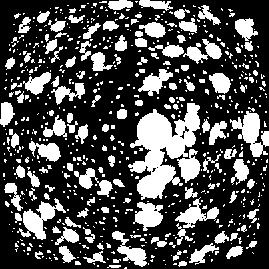
\includegraphics[scale=0.8]{baking.png}
%\caption{Corte del volumen luego de la cocción. Las burbujas siguen un campo vectorial concéntrico.}
%\label{FigBaking}
%\end{center}
%\end{figure}


%\subsection{Intervención Humana en el Proceso}

%\subsubsection{Mean Value Coordinates}

%Para permitir una interacción con el modelado del pan sintético, se definen puntos de control que el usuario puede mover a voluntad para deformar localmente la masa. Para esto se utiliza Mean Value Coordinates (MVC), el cual es un método poderoso en animación \cite{Floater2003,Floater2005,Ju2005}.
%Este método computa coordenadas baricéntricas a partir de los puntos de control sin deformar (una caja que rodea al objeto) con las cuales calcula las posiciones destino de los puntos de interés en el dominio (en nuestro caso, cada pixel de la imagen es un punto de interés).

%El método usa dos conjuntos de puntos de control para realizar la deformación. El primero ($cageOrig$) es un conjunto de puntos que se sitúa en el borde de la imagen original. Cada texel computa su coordenada baricéntrica con respecto a estos puntos. Cuando movemos estos puntos formamos el vector $cageNew$. Para cada píxel $(x,y)$ el método computa las coordenadas baricéntricas del mismo con respecto a la caja original, multiplicando las mismas con los puntos de control deformados. El resultado $(u,v)$ se utiliza como coordenadas en la imagen original para setear el valor que debe tomar el píxel actual:
%\begin{align}
%barycoords &= bary([x,y],cageOrig),\\
%(u,v) &= \sum_{i} {barycoords_{i} * cageNew_{i}}, \\
%T_{new}(x,y) &= T_{orig}(u,v).
%\end{align}
%As the reader will see in next sections, this method produces realistic-looking deformations.

%====================================================================

%Durante el proceso de fabricación del pan, la masa sufre transformaciones que incluyen la intervención del ser humano, el cual busca distribuir la levadura de manera homogénea por medio de deformaciones.

%En nuestro modelo, permitimos que un artista pueda definir puntos de control en una imagen para modificar la silueta externa de la masa. Siguiendo el modelo cilíndrico, la deformación en esta etapa se aplica a cada corte $2D$ del volumen.

%La Figura~\ref{FigMVC} muestra un ejemplo de deformación utilizando Mean Value Coordinates. En este caso se necesitaron solamente $11$ puntos de control (rojo) para aproximar la silueta de la corteza. La FIgura~\ref{FigMVCpoints} muestra los puntos de control y la caja deformada En el ejemplo definimos un mayor número de puntos de control en la región de interés (derecha) para producir una silueta más controlada.

%\begin{figure}[!ht]
%\includegraphics[scale=0.65]{warping.png}
%\caption{Comparación entre pan real (izquierda) y sintético utilizando la deformación por MVC (derecha).}
%\label{FigMVC}
%\end{figure}


%\begin{figure}[!ht]
%\includegraphics[scale=1.35]{warppoints.png}
%\caption{Imagen deformada utilizando MVC: puntos de control sin modificar (verde) puntos de control modificados (rojo). Otras líneas indican desplazamiento de puntos. }
%\label{FigMVCpoints}
%\end{figure}


%This method also warps the bubbles' shape. The deformed bubbles have a natural appearance in concordance with real bread bubbles. 
\section{Conclusiones}
En este Cap\'itulo hemos introducido diversos algoritmos para subsanar la falta de procedimientos flexibles e intuitivos para modelar determinados materiales, entre ellos materiales porosos como el pan. Además, como subproducto de la investigación, se obtuvieron representaciones bidimensionales de madera, granito, mármol y otros materiales comunes en la literatura.
Hemos demostrado visualmente la capacidad de los métodos.

El primer aporte es un algoritmo que produce texturas bidimensionales de materiales conocidos como madera y granito, utilizando sistemas de partículas, el cual fue presentado en una conferencia local \cite{Baravalle2011}.

Haciendo hincapié en materiales porosos, particularmente el pan, diseñamos algoritmos que utilizan sistemas de partículas en conjunción con Sistemas Dinámicos para producir texturas que representan de manera realista geometrías de pan, el cual fue presentado en un congreso y revista nacionales \cite{Baravalle2014}.

Finalmente, utilizando como referencia el proceso de formación real del pan, utilizamos conocimientos de ingeniería de los alimentos para producir una secuencia de pasos que emulan el proceso real de formación del pan.
El mismo permite modelar de manera realista tipos de panes arbitrarios, produciendo geometrías de su miga y su corteza, utilizando un proceso fractal de generación.
Para ello, emulamos un proceso de leudado configurable por el usuario, tanto en forma global, supliendo una geometría arbitraria en tres dimensiones, como en el burbujeado interno, por medio de parámetros intuitivos de generación (radio máximo y mínimo de las burbujas, cantidad de burbujas, etc.).
Luego aplicamos una simulación física de la cocción que deformó ligeramente las burbujas.
Finalmente, la corteza fue generada sobre la superficie del material.
El algoritmo de renderizado utilizado será explicado en el siguiente capítulo, el mismo produjo imágenes realistas de diversos tipos de pan, en varias etapas del proceso de formación del mismo.

El modelo introducido es más flexible y poderoso que el estado del arte actual en modelado de geometría de materiales porosos y panes.

En un capítulo posterior, y con intención de validar el procedimiento, mostraremos que las geometrías obtenidas por el método inspirado en el proceso de formación del pan, arrojan distribuciones de burbujas coincidentes con panes reales.

 \cleardoublepage

\chapter[Renderización de la geometría de Panes]{Renderización de la geometría de Panes y otros Materiales Porosos}
\section{Introducción}
Debido a las limitaciones existentes actualmente en el renderizado realista de pan, nos proponemos en este capítulo estudiar la utilización de renderizado directo de volúmenes aplicado a un campo escalar representando la geometría de la miga de pan. 

%Los resultados obtenidos son realistas y se renderizan en tiempo real. La misma evita el uso de estructuras intermedias, simplificando el desarrollo y reduciendo los costos computacionales.
El renderizado foto-realístico de materiales con una estructura interna compleja presenta grandes retos en Computación Gráfica.
En particular, las migas de panes son un material translúcido complejo, con una estructura porosa, que presenta detalles diferentes en distintas escalas, todos igualmente necesarios de ser tenidos en cuenta para lograr una correcta visualización.
El renderizado realista de estos materiales debe simular correctamente diversos fenómenos como translucencia, auto-sombreado, auto-oclusión, reflectancia, y absorción, entre otros.

Las técnicas del estado del arte en renderizado de migas de panes tratan el material como una superficie, seteando un complejo procedimiento de captura, en el cual la luz reflejada por el material es fotografiada en distintos ángulos.
Luego, la información es procesada y reconstruída para formar un modelo del material.
Si bien esta solución es capaz de capturar los fenómenos lumínicos previamente discutidos, también es cierto que la practicidad del método está severamente comprometida, ya que presenta un costo computacional alto, un procedimiento de captura muy limitado y la imposibilidad de obtener más de una apariencia con una única captura.

En un intento por superar estas limitaciones del renderizado, proponemos, en conjunción con el capítulo anterior de modelado de la geometría, utilizar un modelo volumétrico del pan.
Para esto utilizamos la técnica de renderizado directo de volúmenes, implementada en GPU.
La técnica permite renderizar los campos escalares del capítulo anterior sin utilizar estructuras intermedias.
Las imágenes obtenidas son promisorias, y se computan en tiempo real gracias al poder de las placas gráficas actuales.

\section{Trabajo Previo}
El tópico de renderizado foto-realista de materiales, y su modelado, atrajo un interés creciente en la literatura científica.
La mayoría de los esfuerzos están focalizados en materiales complejos de frecuente aparición como el agua \cite{Schechter2012}, la piel humana \cite{Donner2006}, metales, plásticos \cite{Kurt2010}, etc.
La comunidad de investigadores, sin embargo, ha tenido grandes dificultades para simular adecuadamente la apariencia de otros materiales, como es el caso de materiales cocidos ({\em e.g.}, pizza, galletitas).
Debido a su compleja geometría y fenómenos lumínicos involucrados, esto continúa siendo un problema abierto \cite{Voglsam2013}.

Hasta hace pocos años, el costo computacional de renderizar modelos físicos de estos materiales resultaba prohibitivo si el tiempo real era un requerimiento.
De todas formas, el crecimiento notable en poder de cómputo debido al diseño masivamente paralelo de las placas gráficas \cite{Yeo09,Harris06}, está permitiendo la simulación de complejos fenómenos de interacción de la luz con los materiales en tiempos de cómputo aceptables.

Simulating an acceptable bread geometrical model represents an additional challenge.
This and other kinds of porous structures are the result of complex mechanisms involving physical deformations, heat and mass transport during baking, and several chemical reactions.

Recent studies employs phenomenological considerations on real breads, but the geometry is fixed ({\em i.e.}, non procedural) \cite{VanDyck2014}: a fixed geometry does not allow to obtain several different bread types easily, since it requires a capture procedure for each of them, and, in addition, bubble distributions can be neither controlled nor changed.

%Different rendering algorithms are targeted to different data structures. Particularly, triangular meshes should be derived from voxel data (marching cubes \cite{Lorensen1987}). Nevertheless, the construction of a porous bread structure can demand large amounts of memory.

The presence of mesostructures (bubbles and alveoli of complex shapes) makes bread a quasi homogeneous material \cite{Tong2005}. 
For this reason, adequate surface representations of this material are not possible.
Typical techniques such as Bidirectional Reflectance Distribution Functions (BRDFs)
\cite{Kurt2009}, and Bidirectional Surface Scattering Reflectance Distribution Functions (BSSRDFs) \cite{Donner2009}, are not satisfactory.
A material model \cite{Tong2005} solves these limitations, but the associated drawbacks (complex capture procedure involved, computational costs, poor geometry variability),
makes the method far from practical.

On the other hand, research on physically inspired mathematical models of bread crumbs is not uncommon in the food industry related literature.
These works aim to adequately model and simulate heat and mass transfer in dough during baking, among other issues.
Recent results suggest that 1D models could suffice, for instance modeling the geometry as an infinite cylinder, or assuming only one radial coordinate \cite{Purlis2012, Thorvaldsson1999}.
These and other results in the food industry have some significance in bread crumb modeling and rendering, and may be used as a further basis for computational baking models. 


\section{Renderizado Directo de Volúmenes (DVR)}
The technique of Direct Volume Rendering (DVR)\cite{Kratz2006} generates two-dimensional images by computing the interaction of light with a semi-transparent medium that is represented by a discrete scalar field.
This field describes the density of the medium at regular sample points. 
For each pixel in the image a ray is cast from the camera position and the radiance reaching the camera from its direction is computed by approximating the radiative transfer equation (RTE). This equation describes the change in radiance along a ray as it traverses non-transparent media.
In its complete form, the RTE incorporates many different optical properties and effects. 
In order to approximate the result of the RTE in real-time, this work uses a simplified version of the equation that only incorporates some of the optical phenomena that occur in reality.

There are three important optical phenomena that affect the propagation of light through a medium at a given point in space: emission, absorption and scattering.
Emission is the generation of radiant energy in a given direction.
Absorption happens when a fraction or all of the radiant energy in the light ray hits an opaque object and is transformed into other forms of energy. 
%
Finally, scattering events result in the change of direction of photons. 
Scattering events that cause photons to change directions away from the direction of a ray are called out-scattering events. Conversely, in-scattering events result in photons changing direction towards the ray direction.
%
The contribution of in-scattering is often computed for radiance from a single direction which corresponds to the main light source of the scene.
This corresponds to the radiative energy arriving at a point from the light source, bouncing on the particles in the medium at that point and then traveling along a given ray direction.

The RTE can be summarized as:

\begin{equation} \label{eq:general_radiance}  
  L(p_n) = L_b + \int_{p_0}^{p_n} \frac{\partial L(t)}{\partial p} \, dt,
\end{equation}

\noindent where $L_b$ is the background radiance, and $p_0$, $p_n$ are the closest and furthest visible points along the ray direction, respectively, $L(t)$ is the radiance at point $t$, and $\partial p$ is the distance between sampled points. 
Since the input to the DVR algorithm is a discrete data set, in order to compute $L(p_n)$ the integral is approximated by a sum.

Extinction is the decrease in radiance in a ray due to absorption and out-scattering.
We can approximate this effect by defining an absorption coefficient for the media, $k_a$ and an out-scattering coefficient $k_s$. 
If we neglect the out-scattering effect, the formula that describes the radiance reaching a point after traversing a ray segment is:

\begin{equation} \label{eq:radiance_absorption}  
    L_b \ e^{- \textstyle  \int_{p_0}^{p_n} k_a(t) \, dt}.
\end{equation}

We introduce the value $\int_{p_i}^{p_j} k_a(t) \, dt$, the absorption coefficient, and we will refer to it as $\tau_{(p_i, p_j)}$. 
Transmittance is complementary to extinction. It describes the amount of light passing through a medium in a given direction. 
The transmittance value along two points $p_i$ and $p_j$ is thus:

\begin{equation} \label{eq:transmittance}  
  T(p_i,p_j) = e^{- \textstyle \tau_{(p_i, p_j)}}.
\end{equation}

If we assume that at every point inside the volume along the ray there is an increase of radiance due to emission and in-scattering phenomena ($\rho$), then our initial radiance estimate becomes:

\begin{equation} \label{eq:ray_radiance}  
  L(p_n) = L_b \ e^{-\tau(p_0, p_n)} + \int_{p_0}^{p_n} \rho \ e^{-\tau(t,p_n)} \, dt.
\end{equation}


This means that the radiance along points $p_0$ and $p_n$ is the attenuated remaining background radiance plus the attenuated emission and in-scattering at every ray point.
The DVR algorithm samples the volume density function at regular intervals, approximates the transmittance along those points and computes the amount of light reaching the camera along the ray direction.
The computation replaces the integral sum by a discrete sum over the length of the ray intersecting the volume:

\begin{equation} \label{eq:ray_radiance}  
  L(p_n) = L_b \ e^{-\tau(p_0, p_n)} + \sum_{p_0}^{p_n} \rho \ e^{-\tau(p_i,p_n)}.
\end{equation}

Other effects can be accounted for, augmenting the final image's fidelity, as well as the technique's computing cost. 
The basis of our rendering algorithm uses the simplified transmittance and emission only model, along with some artistic considerations, to achieve real time frame rates.
The rendering algorithm is described in detail in a further section. 
%~\ref{sec:rendering}.
%%%%%%%%%%%%%%%%%%%%%%%%%%%%
%La técnica de DVR tiene como objetivo crear una representación bidimensional de un volumen
%definido por una función de densidad tridimensiopocnal. Para ello, se emiten rayos desde el punto de vista de una cámara en una escena virtual y se utiliza la función de densidad para calcular la cantidad de luz que la cámara recibe en la dirección del rayo. Para esto se evalúa la función de densidad en el camino del rayo y se usan los valores adquiridos para aproximar el efecto de varios fenómenos lumínicos, como pueden ser la extinción, transmitancia, o dispersión lumínica, entre otros. La información obtenida de procesar todos los rayos se utiliza para definir el color de los pixeles en la imagen final.

%La radiancia es la cantidad de luz que pasa, o es emitida, desde un punto y atraviesa un determinado ángulo sólido. En el contexto de DVR, el medio que los rayos atraviesan, y que es definido por una función de densidad, es considerado como emisivo. Por lo tanto, cuando se busca calcular la cantidad de luz recibida en la dirección de un rayo, lo que se hace es aproximar la radiancia recibida de un punto distante siguiendo la dirección del rayo. El valor de la radiancia es aproximado como la suma de una radiancia de fondo y la radiancia emitida por el medio por el cuál se mueve el rayo \cite{Kratz2006} :

%\begin{equation} \label{eq:general_radiance}  
%  L(p_n) = L_b + \int_{p_0}^{p_n} \frac{\partial L(t)}{\partial p} \, dt,
%\end{equation}

%\noindent donde $L_b$ es la radiancia de fondo, $p_0$ y $p_n$ son los puntos inspeccionados en la dirección del rayo más cercano y más lejano respectivamente, $L(t)$ es la radiancia evaluada en el punto $t$, y $\partial p$ es la distancia entre puntos evaluados. En el momento de calcular $L(p_n)$, la integral es aproximada por una suma.

%La extinción es la pérdida de fotones en un haz de luz debido a la absorción en el medio que atraviesa y la dispersión hacia otras direcciones. Algunos de los fotones colisionarán con particulas del medio y serán absorbidas y transformadas en otras formas de energía, mayormente calor. Otras rebotarán y pasarán a moverse en otras direcciones. Estos fenómenos se aproximan usando un coeficiente de absorción para el medio, $k_a$ y un coeficiente de dispersión $k_s$. Si el efecto de dispersión es ignorado, la fórmula que define la cantidad de radiancia absorbida en el largo de un segmento de rayo
es: 

%\begin{equation} \label{eq:radiance_absorption}  
%    L_b \ e^{- \textstyle  \int_{p_0}^{p_n} k_a(t) \, dt}.
%\end{equation}

%El valor $\int_{p_i}^{p_j} k_a(t) \, dt$ es llamado coeficiente de absorción y se referenciar\'a como $\tau_{(p_i, p_j)}$.

%La transmitancia es un concepto complementario a la extinción y describe la cantidad de luz que pasa por un medio en una dirección determinada. El valor de transmitancia entre dos puntos $p_i$ y $p_j$
%es:

%\begin{equation} \label{eq:general_radiance}  
%  T(p_i,p_j) = e^{- \textstyle \tau_{(p_i, p_j)}}.
%\end{equation}

%Si la emisión de luz se asume como un término constante ($\rho$) para todos los puntos del medio, la fórmula inicial de radiancia queda:

%\begin{equation} \label{eq:ray_radiance}  
%  L(p_n) = L_b \ e^{-\tau(p_0, p_n)} + \int_{p_0}^{p_n} \rho \ e^{-\tau(t,p_n)} \, dt.
%\end{equation}

%Esto significa que la radiancia entre los puntos $p_0$ y $p_n$ se puede calcular como la radiancia de fondo restante luego de la atenuación del medio sumada a la emisión, también atenuada, en todos los puntos del medio que atraviesa el rayo.

%La técnica de DVR define un volumen donde una función de densidad se evalúa en intervalos regulares y utiliza esa información para aproximar la transmitancia en esos puntos y de esa manera aproximar la cantidad de luz que llega a la cámara. La suma integral descrita anteriormente se reemplaza por una suma discreta de los puntos evaluados de un rayo donde \'este intersecta al volumen que interesa representar. 

%Otros efectos lumínicos pueden ser aproximados. Esto aumenta la fidelidad de la imagen final pero también aumenta el costo de cómputo de la técnica. Algunos de estos efectos son el cálculo de fase, el c\'alculo de luz entrante por dispersión o luz extinguida por dispersión, entre otros. Dado que el objetivo de este trabajo es lograr un renderizado en tiempo real, el algoritmo implementado usa como base el modelo de cálculo de radiancia simplificado que toma en cuenta sólo la
%transmitancia del medio.

\section{Implementación}


We created a demo application \footnote{available at \emph{https://www.github.com/rbaravalle/Pysys}} that uses the particle system described in the previous sections to render real-time bread models using a DVR approach. 
In this demo we produced a volume texture from the original particle system.
A cube that corresponds to this volume is then rendered in the scene.
The material used to render the cube uses a very simple vertex shader and a fragment shader that implements the DVR algorithm. For each fragment, this shader computes a ray originating from the camera position and in the direction of the fragment that must be shaded. 
The procedure samples the volume texture at regular intervals along the intersection of this ray and the cube.
The sample values are then used as input of a simplified version of the radiative transfer equation to compute the resulting pixel color as described in previous sections.
%~\ref{sec:DVR}.
We employ these equations to accumulate the transmittance of the ray and the radiance contribution at every sample point.
The computation ends if the transmittance falls below a threshold value or if the ray exits the cube. 
Single in-scattering is approximated by computing a secondary ray at each sample point directed towards the scene light source.
This secondary ray is then sampled to determine the amount of light that reaches the original sample point. 
This technique allows to naturally perform self shadowing within the model.

We shade the pixel using the primary and secondary ray transmittance information. 
At this point, different artistic considerations may be applied to yield different
looking materials.
For instance, we can differentiate crumb and crust by assigning a higher extinction coefficient and a darker color to crust regions. 
A soft yellowish color applied in other regions provides a crumb appearance.
Additionally, it is possible to add a faint specular reflection. 
The contribution of that reflection is computed at the first intersection point between the ray and the particle system in order to increase the final image realism. 
The normal vector used for this computation is the gradient of the volume texture at that point.

The demo we present provides the user with the ability to modify parameters such as the transmittance coefficient, the transmittance threshold, the color assigned to the crumb and the visibility of the specular highlights. 
By modifying these parameters the user can produce images that resemble other porous materials, such as sponges.

\subsection*{Ambient Occlusion}

One key aspect to enhance the final image appearance is the local contributions due to tiny material features (emission, occlusion, absorption). 
Previous works show that considering ambient occlusion can greatly enhance synthetic image realism \cite{Hernell2010}.
Based on this idea we approximate multiple in-scattering by computing (offline) an ambient occlusion term for each voxel in the scalar field and storing it as an additional volume texture, which is used by the fragment shader.

For each voxel, the algorithm sets a neighborhood of radius $r$ and stores the mean voxel value within that radius in the ambient occlusion texture.
It then uses this value to modulate the contribution of a ray sample.
Setting different values for $r$ produces similar results. 
Fig.~\ref{fg:occlusion} shows that the enhancement added using ambient occlusion clearly improves the final image appearance and is a key aspect in realistic bread appearance. It is worth mentioning that the net effect of this term was somehow oblivious to the radius $r$ of the surrounding sphere, for $r > 0$.
 
\subsection*{Normals Computation}

We use a simple forward difference schema for the gradient computation. In this method, we compute the normal vector at a point using the gradient, represented as the normalized difference vector between the field values at the forward positions and the actual position:

\begin{equation}
\begin{aligned}
x &= tex(pos+(1,0,0)) - tex(pos)\\
y &= tex(pos+(0,1,0)) - tex(pos)\\
z &= tex(pos+(0,0,1)) - tex(pos) \\
N &= normalize([x,y,z])
\end{aligned}
\end{equation}

We use the normals and the light vector to determine the specular contribution, applying a simple Phong model \cite{Phong1973}, with a parameter that lets the user change the impact of the specular component.
We tested other more accurate specular models, but there was no appreciable difference in the final bread appearance.

\subsection*{Shadows Computation}

The DVR technique can also be used to compute realistic shadows using shadow maps \cite{Williams1978}.
During the shadow map generation we again render a cube representing the particle system.
The fragment shader for that box uses the same ray-casting method explained above, but only computes the transmittance along the ray. 
If the transmittance along the ray is above a threshold value, then the fragment does not correspond to an occluder and its depth is set at infinity. 
If during the volume traversal the transmittance falls below the threshold, the fragment depth is set to that sample point depth.
This technique is used along with percentage-closer filtering to generate realistic looking shadows in our demo application.

\subsection*{Crust}
We can provide a function that defines whether a volume point is part of the crust or the crumb. For instance, we may provide a function that defines a cylindrical crust envelope by assigning crumb to positions close to the axis of the cylinder, and crust to all other positions. Another function is provided to define whether a point should be considered empty air.
This allows an easy way to define bread crust and slices (see Figs.~\ref{fg:crumb} and \ref{fg:results2}).

\paragraph{Crust determination using Mathematical Morphology}
Since it is difficult or impossible to define mathematical functions that adapt to arbitrary shapes, we propose an automatic method for crust determination using mathematical morphology \cite{Gonzalez2001}.
The idea is to obtain an outer region of the resulting $3D$ scalar field. 
For this, we use basic techniques known as closing, erosion and dilation.

For the purposes of our work, we will define the operations on $3D$ binary scalar fields.
A structuring element $E$ is defined as a binary scalar field representing a particular shape (cube, sphere, etc.).
Structuring elements are employed to perform morphology operations.

The erosion operation can be employed to reduce the total size of a scalar field.
The erosion of a $3D$ scalar field $A$ using a structuring element $B$ is defined as:

\begin{equation}
A \ominus B = \{z\in \mathbb{Z}^3 | B_{z} \subseteq A\},
\end{equation}

\noindent where $B_{z}$ is the translation of $B$ by the $3D$ vector $z$.

The dilation operation is used to augment the total size of a scalar field following its boundary.
The dilation of a $3D$ scalar field $A$ using a structuring element $E$ is defined as:

\begin{equation}
A  \oplus E = \bigcup_{e\in E} A_e.
\end{equation}

The closing operation is used to fill holes in the scalar field.
The closing of a $3D$ scalar field $B$ using a structuring element $E$ is defined as a dilation followed by an erosion:
\begin{equation}
B \bullet E = (B \oplus E) \ominus E,
\end{equation}
see \cite{Gonzalez2001} for further details.

To obtain the outer region of the $3D$ porous volume, we have to eliminate the holes in the scalar field (bubbles) and then compute a boundary.
To do this, the first step performs a closing $c$ of the scalar field using a cube (structuring element of radius $r$), causing the closing of interior bubbles.
Calling $d$ the dilation of $c$ with an spherical element of radius $r_{2}$ and $e$ the erosion $d$ using a spherical structuring element with a slightly shorter radius ($r_{3}$).
The difference between $d$ and $e$ lies in the boundary of the scalar field, so it could be used as a crust.
To eliminate some possible inaccuracies resulting from previous steps, we successively perform a closing of $d-e$ and a dilation to the result, obtaining the final crust.
Fig.~\ref{fg:crusts} shows examples of scalar fields with crusts added using this technique. The results naturally adapt to any scalar field, even with holes.
Since the result would completely cover the scalar field, the crust can be set to span only a subset of the complete volume, allowing the user to see the bread crumb.

%%%%%%%%%%%%%%%

%Se cre\'o un programa de prueba\footnote{disponible en \emph{\url{https://www.github.com/rbaravalle/Pysys}}} para evaluar el sistema de partículas que describe la estructura del pan. Este programa usa un campo escalar representando la miga de pan para generar una textura volumétrica que se interpreta como una función de densidad. Esta textura precomputada se usa como entrada para un motor gráfico que utiliza la técnica de DVR para generar imágenes del pan representado por el sistema de partículas original. Este programa demuestra que el método de renderizado propuesto es compatible con los motores gráficos basados en técnicas de renderización en tiempo real en GPU. Se obtienen imágenes de un material realístico así como efectos de sombras suaves dentro del volumen. Esto significa que las técnicas usadas para renderizar estos materiales pueden ser integradas en cualquier motor de renderizado que soporte shaders.

%La malla que utiliza el modelo es un cubo que contiene el volumen definido por el sistema que genera la miga del pan. El código del shader de vértices es muy simple, proveyendo sólamente información geométrica al shader de fragmentos. Este último es donde se encuentra la mayor parte de los cálculos a realizar.

%Dentro del shader de fragmentos la primera operaci\'on es calcular la geometría de un rayo cuyo origen es la cámara de la escena y cuya dirección lo lleva hacia el fragmento siendo calculado. Este rayo es recorrido en intervalos regulares, evaluando la textura volumétrica para obtener la densidad del pan en esos puntos. Este valor se utiliza para calcular la transmitancia acumulada desde la cámara hasta el punto evaluado. Una vez que la transmitancia es menor que un valor preestablecido o el rayo sale del cubo que define el volumen, el cómputo termina.

%En cada punto evaluado también se computa la transmitancia dentro del volumen desde el punto hacia la fuente de luz en la escena. Esto se hace emitiendo un rayo desde el punto con dirección a la luz y nuevamente calculando la densidad en varios puntos del rayo. Con esta nueva información se aproxima la cantidad de luz que llega directamente al punto considerado, y permite representar sombras dentro del volumen.

%La información de transmitancia de los puntos evaluados del rayo principal y desde estos puntos hacia la luz se utilizan para calcular el color final del fragmento. A partir de esta información y tomando diferentes consideraciones artísticas pueden lograrse representaciones realísticas de diferentes materiales. En el caso de las imágenes de muestra presentadas en este trabajo el color del fragmento será más oscuro para areas del volumen que se consideran dentro de la corteza del pan y será de un color amarillo claro para la miga. También se usa un componente especular tenue. La información de transmitancia entre los puntos evaluados y la luz ayuda a proveer detalles de la estructura del pan. La Fig~\ref{fg:fragmentshader} muestra un esquema del cálculo del color final del pixel.

\begin{figure*}[htb!]
  \centerline{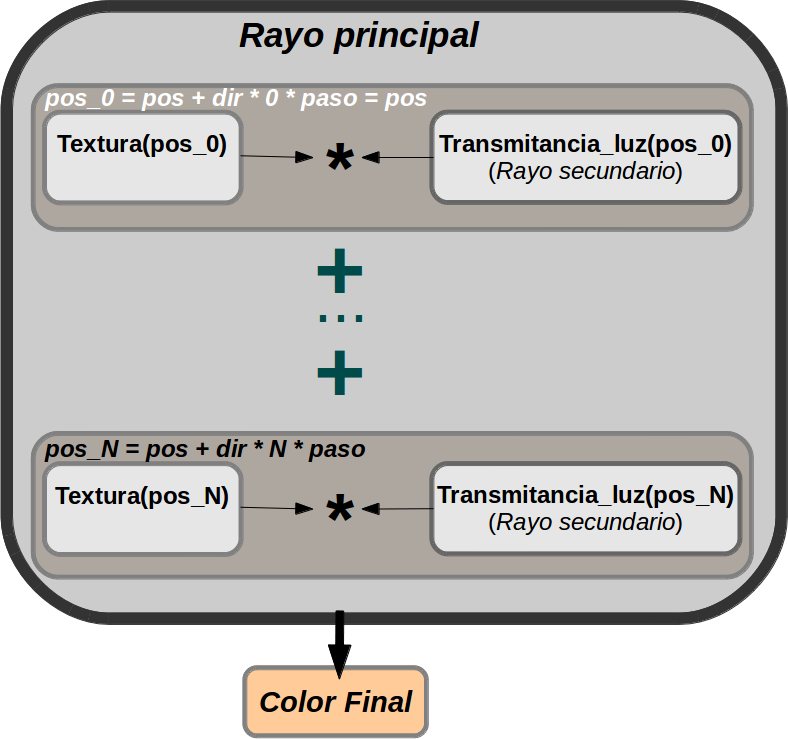
\includegraphics[width=13cm]{fragmentshader}}
  \caption{Cálculo de color en el shader de fragmentos. }
  \label{fg:fragmentshader}
\end{figure*}


El programa de prueba creado permite modificar parámetros tales como el coeficiente de transmitancia del pan, el límite de transmitancia, el color asignado a la miga y la intensidad de los reflejos especulares, entre otros. Esta capacidad permite crear imágenes que semejan otros
materiales porosos, como por ejemplo esponjas.

%\paragraph{Corteza, fetas y cortes}

%Las partes del volumen pertenecientes a la corteza y a la miga del pan fueron determinadas manualmente mediante una función que asigna una u otra propiedad a cada punto del volumen a partir de su posición. Por ejemplo, para volúmenes de forma cilíndrica se definió una función que designa como corteza a los puntos que están a más de una distancia predefinida del eje del cilindro.

%De la misma manera se define una función que determina si puntos del volumen deben considerarse vacíos, independientemente del valor de la textura volumétrica en ese punto. Esto permite definir fetas de pan de manera sencilla. Un ejemplo del uso de este mecanismo puede apreciarse
%en la Fig.~\ref{fg:fig5}.

%La asignación de vacío y de corteza deben ser extendidos más allá de ecuaciones basadas en posiciones para poder ser usadas en un proceso artístico.

%*MORFOLOGIA MATEMATICA*


%En la siguiente sección se presentan y se evalúan los resultados obtenidos.
%
%En esta sección se detallan las imágenes y los tiempos de renderizado obtenidos. 

\subsection{Resultados del renderizado}

%Las imágenes obtenidas a partir del método descrito en la sección anterior fueron renderizadas en una computadora con una placa gráfica nVidia GTX 480 ($480$ cores), la cual es normalmente de uso hogareño. La CPU fue una Intel(R) Core(TM) i5-2300 CPU (cuatro procesadores). La resolución de las imágenes es de $1440\times990$ pixels. 
%Se obtuvieron diferentes imágenes que semejan materiales horneados. Diferentes tipos de pan pueden ser representados variando los parámetros de transmitancia y colores utilizados (ver Fig.~\ref{fg:fig5}). En la imagen central los patrones producidos por los sistemas de partículas descritos en las secciones previas son claramente visibles. En ese caso, el tiempo de vida de las partículas es diferente para cada una y de esa manera se obtienen burbujas de
%diferentes tamaños.

\begin{figure*}[htb!]
  \centerline{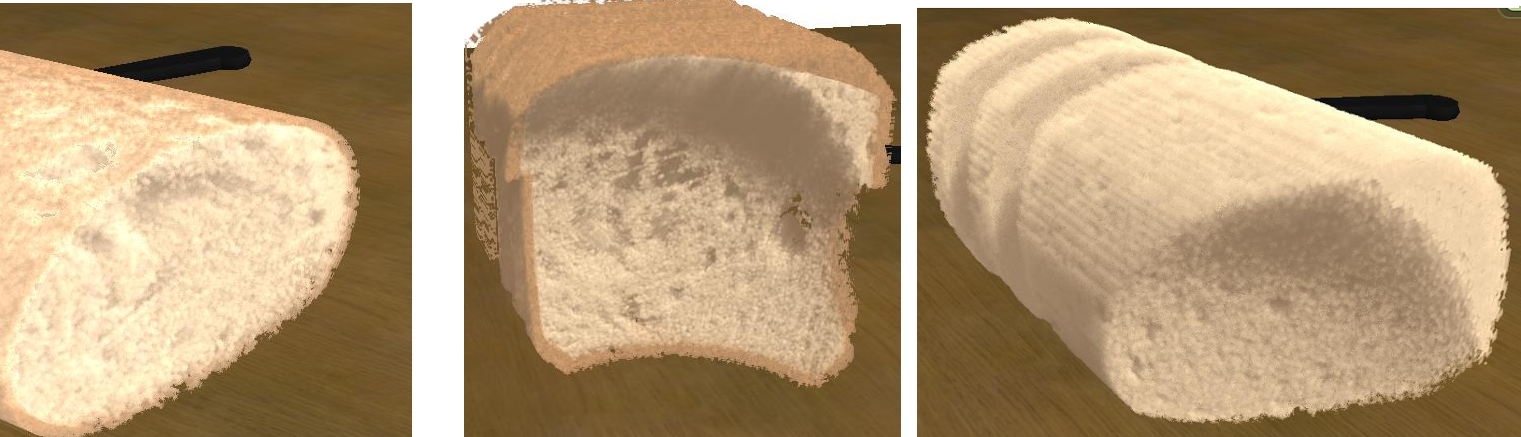
\includegraphics[width=13cm]{fig5}}
  \caption{Imágenes de diferentes tipos de pan renderizados en tiempo real. La imagen de la derecha muestra un pan sin corteza}
  \label{fg:fig5}
\end{figure*}

Es posible obtener otros materiales (ver Fig.~\ref{fg:fig6}). Estos son el resultado de la variación de parámetros técnicos y artísticos del modelo. En las imágenes de prueba pueden distinguirse un budín (izquierda), un pedazo de torta (medio) y una esponja (derecha). En el caso de la esponja se modificaron los parámetros que definen la función de densidad. Cuando no hay levadura en el proceso de creación puede utilizarse una textura volumétrica cuyos valores provienen de una función aleatoria. La retroiluminación es también aproximada con este modelo (ver Fig.\ref{fg:fig7}). En esa imagen puede apreciarse una esponja retroiluminada junto con la propagación de luz a través del volumen que representa.

\begin{figure*}[htb!]
  \centerline{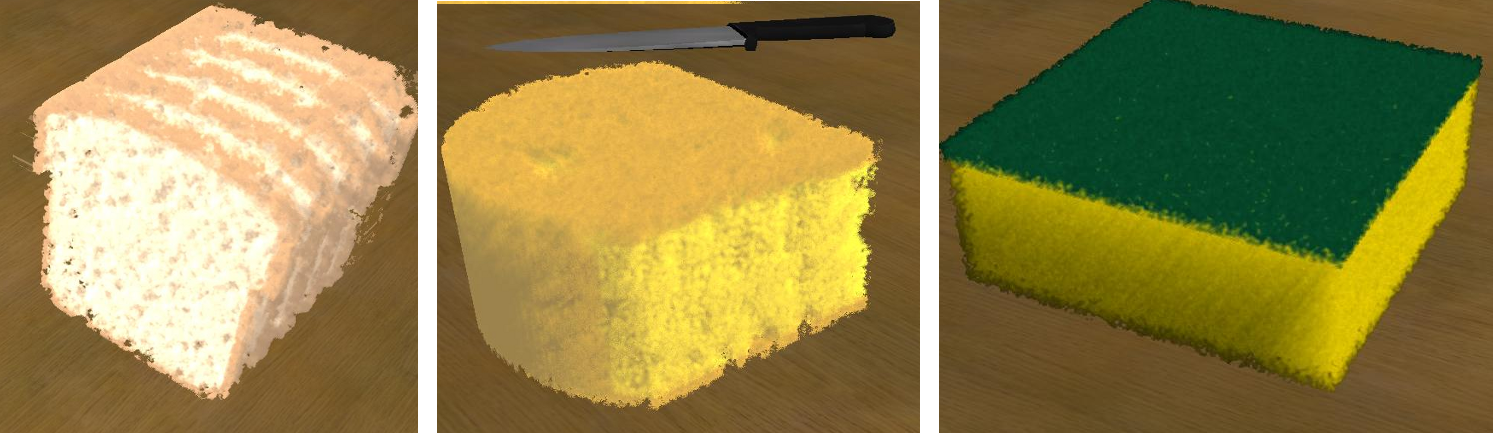
\includegraphics[width=13cm]{fig6}}
  \caption{Distintos materiales obtenidos a partir de diferentes configuraciones de parámetros. De izquierda a derecha: budín, torta y esponja. }
  \label{fg:fig6}

\end{figure*}

\begin{figure*}[htb!]
  \centerline{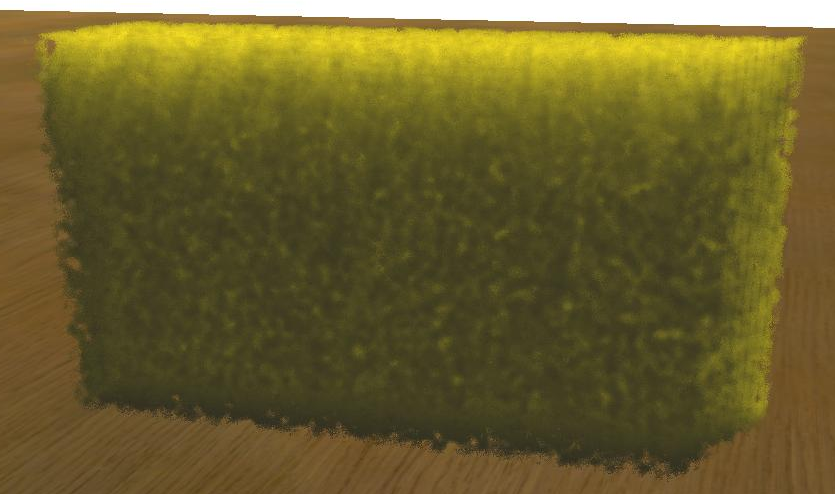
\includegraphics[width=8cm]{fig7}}
  \caption{Esponja retroiluminada.}
  \label{fg:fig7}
\end{figure*}

\subsection{Tiempos de renderizado}

La mayoría de las imágenes se obtuvieron con tasas de refresco de tiempo real (más de 30 FPS), como muestra la Tabla~\ref{tab:n1}. La eficiencia del proceso se resiente cuando la transmitancia es muy baja (el material es casi transparente), dado que se evaluarán más puntos en los rayos a recorrer antes de llegar al límite de transmitancia. Otro parámetro importante es la distancia entre puntos a evaluar. En la Tabla~\ref{tab:n2} se observa que a medida que la cantidad de rayos y de pasos del rayo aumenta, la velocidad decrece. La tabla muestra que los rayos secundarios constituyen el principal cuello de botella, lo cual es lógico, dado que a cada paso del rayo principal, el mismo computa un rayo secundario hacia la luz.

Experimentalmente se encontró que para todos los casos a evaluar $100$ puntos o más presenta buenos resultados.El proceso escala automáticamente con el número de procesadores en una GPU, por lo cual la tasa de refresco obtenida será mayor en GPUs más rápidas y de más procesadores.


ACTUALIZAR!
\begin{table}[htb]
\centering
\begin{tabular}{|c|c|c|c|c|c|c|}
\hline &  Pan 1 & Pan 2 & Pan 3 & Budín & Torta & Esponja \\
\hline
\hline
 FPS promedio  & 32.2 &  75.5 &  45.2 & 28.5 &  54.2 & 29.7\\
\hline
 Puntos de evaluación &  140 &  140 &  140 & 256 &  140 & 256 \\
\hline
 Transmitancia &  15 &  15 &  15 & 15 &  15 & 2.25 \\
\hline
\end{tabular}
\caption{Tiempos de renderizado y parámetros de las imágenes de prueba.}
\label{tab:n1}
\end{table}

\begin{table}[htb]
\centering
\begin{tabular}{|c|c|c|c|c|c|c|}
\hline
 Pasos del rayo         & 128 &  256 \\
\hline
\hline
 Tiempo total shaders   & 10 ms &  32.5 ms \\
\hline
 Rayo Principal         & 2 ms  & 5 ms  \\
\hline
 Rayos Secundarios      &  8 ms & 27.5 ms  \\
\hline
\end{tabular}
\caption{Detalle de tiempos de renderizado en milisegundos.}
\label{tab:n2}
\end{table}


\section{Resultados}
We employed a nVidia GTX 480 ($480$ shader units), which is a typical user configuration.
The CPU is an Intel(R) Core(TM) i5-2300 CPU (quad core).
The screen resolution is $1440\times900$.
In fig.~\ref{fg:application} we show a real-time rendered bread.
Different kinds of bread can be easily modeled changing the parameters of the algorithms (see Fig.~\ref{fg:crumb}).
In Fig.~\ref{fg:results2} we added crust to enhance the final results. 
We also synthesized sponges (see Fig.~\ref{fg:sponges}) with yet different parameter values.
They were easily derived by changing the color and the structure of the volume.
Since yeast is unnecessary in the sponge manufacturing process, we used a random volume texture as a geometry.

We also handled back illumination in the model (see Fig.~\ref{fg:backillum}): the render shows the light propagation in the medium when illuminated from behind.
This is a natural consequence of the RTE based algorithm and the choice of the volume representation that we made.

\subsection*{Computing times}

We rendered all images in real time (FPS over 30). Two parameters are responsible for most of the computations: the transmittance coefficient and the step count.
A low transmittance produces a more transparent material making the ray accumulate more information.

The step count is crucial since for each step we compute the transmittance to the light using a secondary ray.
We experimentally found that values above $140$ give reasonably images for sponges but we needed at least $300$ steps to get a reasonably bread appearance, see Fig.~\ref{fg:stepcount}.
The process automatically scales with the number of GPU processors, so the fps count will increment in more powerful GPUs. 
The use of crust slightly boosts the performance since the transmittance is lower for crust regions, {\em i.e.}, the rays need lower step counts to reach a threshold opacity level.


\section{Otros Materiales Renderizados}

%\section{Conclusiones}

%Según el conocimiento de los autores, éste es el primer intento de llevar a cabo una renderización en tiempo real de pan de manera convincente sin el uso de procesos intermedios complicados (captura de imágenes, generación de mallas, post-procesamiento). Existen buenos resultados de renderizado de pan obtenidos con otros métodos \cite{Cho2007}, pero es difícil comparar ese trabajo con el presentado en este artículo debido a que ni los detalles de la técnica utilizada ni los tiempos de cálculo han sido publicados.

%Dentro del volumen a renderizar se pueden definir regiones con diferentes propiedades. Esta idea permite generar imágenes con miga y corteza con diferentes parámetros.

%La integración de la técnica descrita con motores gráficos es simple. La información de profundidad de los fragmentos puede obtenerse de manera sencilla y por lo tanto pueden utilizarse técnicas populares de sombras, tales como mapas de sombras.

%Los tiempos de cómputo muestran una alta eficiencia del proceso, lo cual depende en gran medida del número de puntos de evaluación usados y la transmitancia del material. Se pueden alcanzcar tiempos de cómputo consistentes con aplicaciones de tiempo real en todos los casos menos en los cuales el volumen ocupa la mayor parte de la imagen a generar, dado que la técnica se calcula casi enteramente en los shader de fragmentos. 

\section*{Discussion}

%1)En primer lugar, un resumen de lo que hicimos en el paper y por qué es importante/novedoso

To the best of the authors' knowledge, this is the first attempt to convincingly render bread crumb and other materials in real time without introducing complex intermediate processes (capture, mesh generation, precomputation, post-process).
There are few previous approaches to bread rendering. An example is \cite{Cho2007}, but comparisons with this technique could not be established since key details are unexplained (computing times, render method).
The proposed method is compatible with current rasterization-based real-time GPU rendering pipelines, providing a realistic looking material, and can be easily integrated into  shader-based 3D engines.
Also, the presented shadow mapping technique allows a natural integration of the volume within scenes. 

%3) Recordamos que las imagenes obtenidas fueron buenas, y que obtuvimos otros materiales cambiando pocos parametros

The modeling and rendering algorithms are flexible enough to model different materials like bread or sponges, changing a few parameters.
Other materials such as cakes, pizzas and cheeses can be implemented in the same way, allowing to manage several materials using the same method.
Also, our volume representation method allows to make real time cuts in the bread crumb.
This is clearly useful in many applications, for instance in video games.

Regarding the illumination model, the success of our algorithms in rendering realistic bread crumbs and other materials could be attributed to the improvements we added to the basic DVR algorithm.
A remarkable improvement in the final realism was due to the addition of an ambient occlusion term, giving the texture a more rich and complex appearance.
Other effects, such as the Phong specular component, enhanced the bread crumb final appearance.
More sophisticated specular methods (for instance, Cook-Torrance model \cite{Cook1982}) did not add a significant improvement.

%5)Tiempos de cómputo (muy importante en este paper!)

Computing times were adequate for real-time rendering in standard off-the-shelf computers (we employed a nVidia GTX 480 GPU with an Intel(R) i5 processor).
Reasonable framerates are always achieved except when the rendered object encompasses a big portion of the screen, since the approach is largely fragment-shader bound.
The final framerate also depends on the step count and the transmittance coefficient.
In addition, different materials require different computing costs for rendering.
For instance, an adequate step count to simulate sponge is lower than the bread crumbs step count.
This can be attributed to the fact that the method needs more steps to capture the macroscopic bread bubbles in crumb.
So far, with current off-the-shelf hardware, our method is limited in the final 3D resolution of the material when real-time applications are required.
In other words, drastic close-ups to the structure could lead to homogeneous areas.
This limitation is tied to the GPU texture size, and will be eventually circumvented with next generations of hardware.
In off-line applications, memory swap procedures allow more satisfactory 3D resolutions.


\section*{Conclusions}

In this paper we applied the transmittance direct volume rendering model using the GPU to a 3D scalar field representing the bread crumb structure, obtaining realistic bread crumb images.
We modeled this structure using particle systems and dynamical systems.
We employed a numerical simulation to solve the resulting set of equations which represents the dynamical system. 
The particles avoided each other and grew following the dynamic system.
The modeling algorithm was easily implemented. 
We implemented the render algorithm in the fragment shader using specular and diffuse components, ambient occlusion and automatic crust determination.

Results showed high fidelity images in real time, suitable for application in several areas, such as video games, serious games \cite{Susi2007} and photorealistic rendering. 
These techniques are much simpler and does not present the drawbacks of other state of the art methods, such as capture processes or mesh generation.
These results make us believe that the volume representation is a right choice for bread modeling and rendering.

As possible continuations of this work, we may extend DVR to handle other phenomena such as indirect illumination, enhancing the resulting images.
Other porous materials such as cheeses will be investigated.
We will employ a number of possible solutions to overcome the resolution problem, such as setting different volume textures depending on the distance between the camera and the volume. 



\begin{figure}
  \centerline{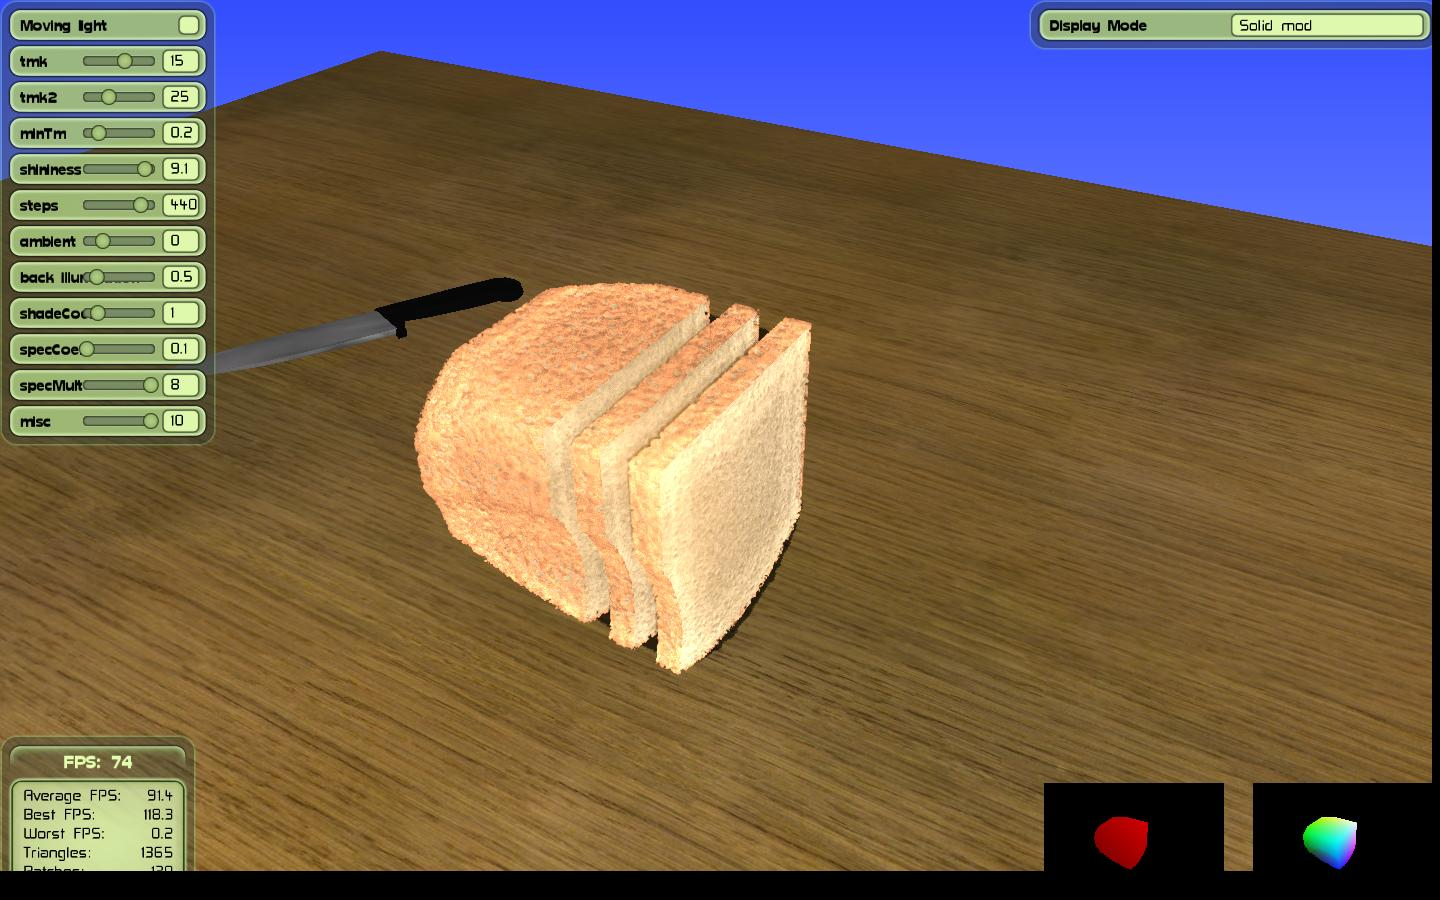
\includegraphics[width=13cm]{figures/application}}
  \caption{Our demo application showing a real time rendered bread.}
  \label{fg:application}
\end{figure}

\begin{figure}
  \centerline{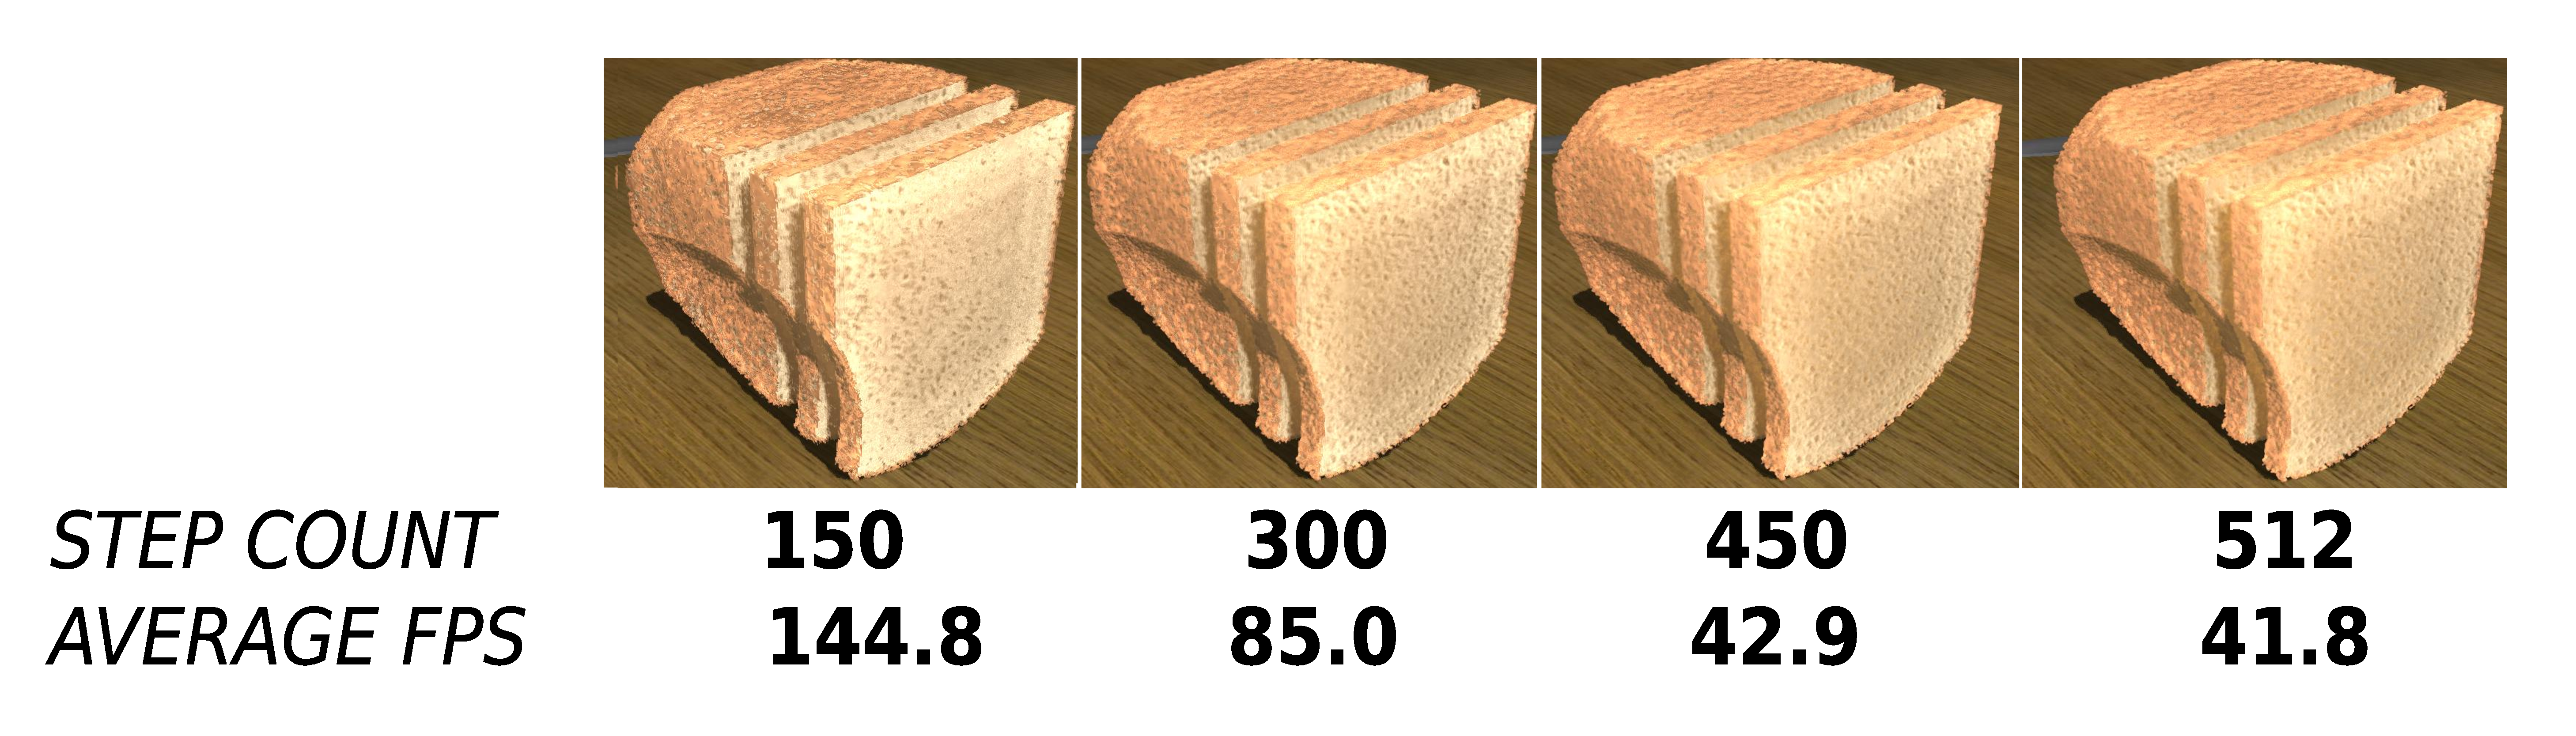
\includegraphics[width=13cm]{figures/stepcount}}
  \caption{Computing times and step count. The image shows that using $300$ sampling ray steps gives reasonably images. }
  \label{fg:stepcount}
\end{figure}

\begin{figure}
  \centerline{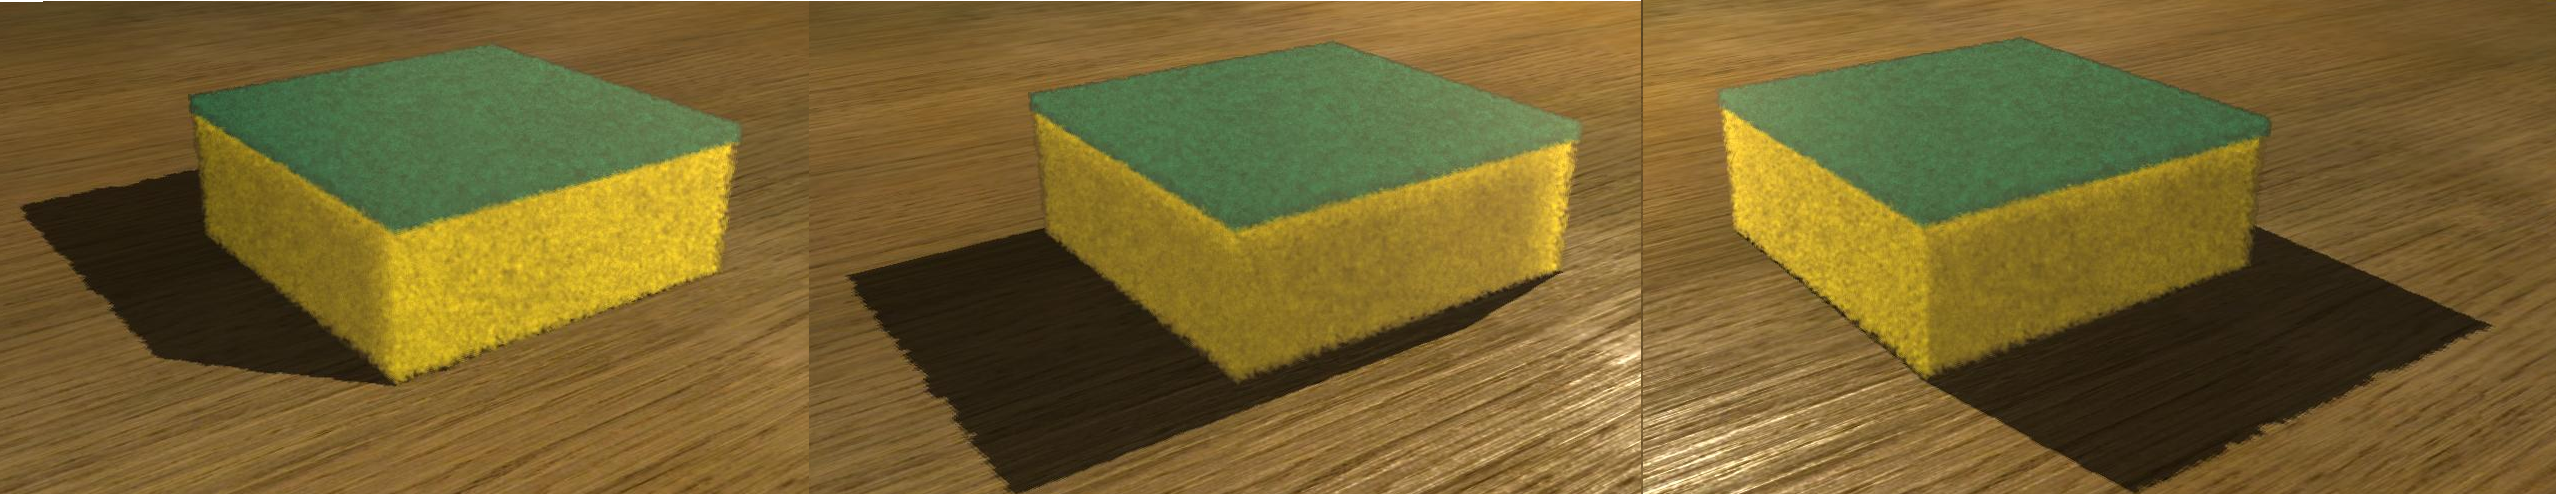
\includegraphics[width=13cm]{figures/sponges}}
  \caption{Real time rendered sponges using a random scalar field as geometry.}
  \label{fg:sponges}
\end{figure}

\begin{figure}
  \centerline{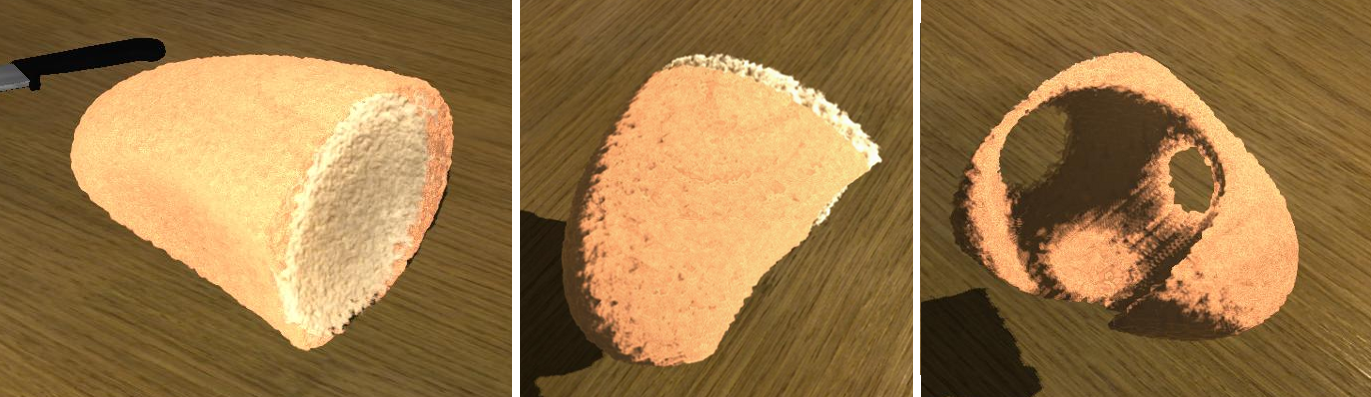
\includegraphics[width=13cm]{figures/crusts}}
  \caption{Crust determination using mathematical morphology. The right image shows that the method works even in extreme cases where the scalar field has holes. }
  \label{fg:crusts}
\end{figure}

\begin{figure}
\centerline{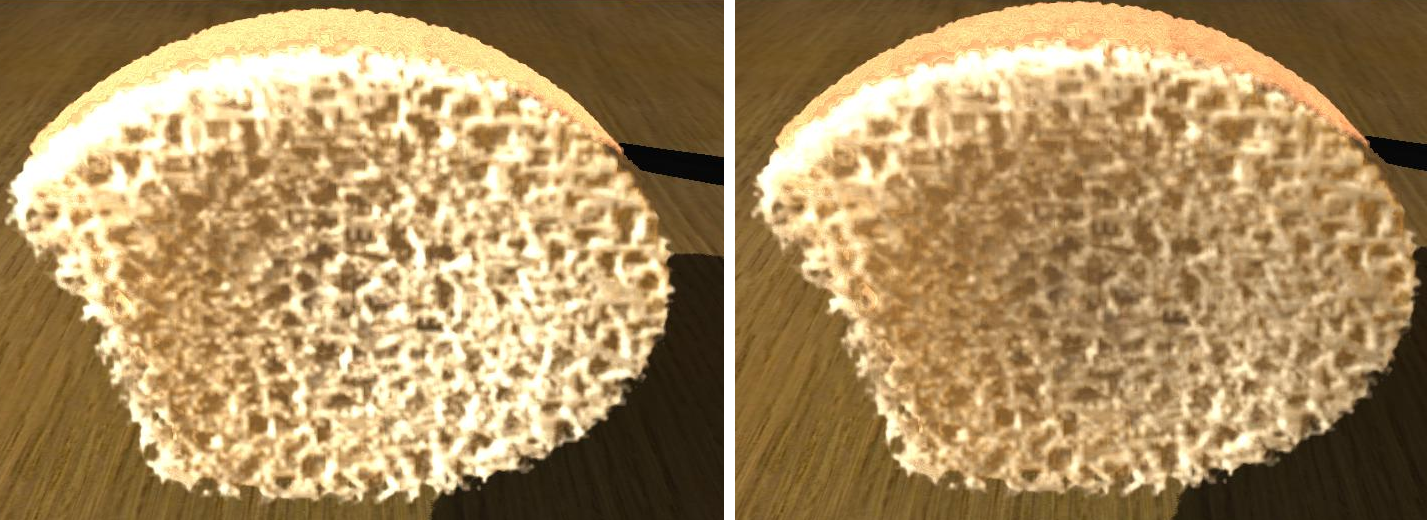
\includegraphics[width=13cm]{figures/occlusion}}
  \caption{Bread without (left) and with (right) ambient occlusion. The final appearance is greatly improved, showing a more natural look. }
  \label{fg:occlusion}
\end{figure}
 \cleardoublepage
\chapter[Características Fractales del Pan]{Características Fractales y Multifractales del Pan}

%\subsection{Características Fractales y Multifractales del Pan}
En esta sección nos proponemos caracterizar distintas muestras de pan por medio de extracción de características.
Gracias a estas t\'ecnicas, podemos validar los resultados obtenidos en los cap\'itulos anteriores con una base matem\'atica s\'olida, m\'as all\'a de la validaci\'on visual realizada por las personas, la cual es utilizada tradicionalmente en computaci\'on gr\'afica.
Además, las características fractales y multifractales capturan características esenciales que pueden ser utilizadas para la clasificación de las muestras, superando a otros clasificadores del estado del arte.



\subsection{Clasificación de Imágenes de Pan Utilizando Características Fractales y Multifractales.}



En esta sección realizaremos una extracción de características útiles sobre la miga de pan, la cual nos permitirá caracterizar la miga y validar los resultados obtenidos.


Se obtuvieron $20$ imágenes de $4$ tipos de panes diferentes ({\em baguette}, {\em lactal}, {\em salvado} y {\em sandwich}, contabilizando $80$ imágenes) utilizando un escáner HP PSC 1210 con los siguientes parámetros de captura:  highlight $190$, shadows $40$, and midtones $1$. Las imágenes fueron obtenidas a una resolución de $380\times 380$ píxeles (el área máxima posible para los $4$ tipos de pan) a una resolución de $350$ dpi ($1$ pixel $= 0.00527$ $[mm^{2}]$). Las mismas fueron convertidas a escala de grises ($8$ bits). Además, se obtuvieron $20$ imágenes de cada tipo de pan utilizando una cámara digital con la misma resolución espacial. Las condiciones de iluminación de estas imágenes son distintas a las de las imágenes del escáner para probar la robustez del método. En la FIgura ~\ref{fig:camera} se observan $4$ ejemplos de imágenes de pan obtenidas con la cámara digital. Además se utilizaron $40$ imágenes de la base de imágenes CalTech101 dataset~\cite{FeiFei04} para introducir imágenes de objetos diferentes al pan y observar la capacidad del método para separar panes de otros objetos.

\subsection{Extracción de Características de Migas de Panes}
Para comprender mejor los valores devueltos con las dimensiones obtenidas, se extrajeron características típicas de las imágenes binarizadas para establecer correlaciones con las dimensiones multifractales.

Se computaron la fracción de vacío de la imagen (FV), el área media de las burbujas (MCA) y el desvío estándar del área media de las burbujas (stCA) para establecer relaciones con la porosidad, granularidad y heterogeneidad de las diferentes migas.

\subsubsection{Binarización de migas de pan utilizando umbralamiento local}
Para determinar las mismas, sólo se utilizaron imágenes binarizadas de las muestras tomadas con el escáner, evitando mezclar imágenes tomadas en diferentes condiciones lumínicas. Las binarizaciones se llevaron a cabo utilizando el algoritmo de umbralamiento local descripto en \cite{White83}. El mismo presentó mejores resultados que la utilización del algoritmo presentado en \cite{Huang95} y utilizado en \cite{Gonzales2008}, el cual utiliza un umbralamiento global de la imagen. Esto se debe a que sutilies variaciones en la iluminación de la misma muestra resultados incorrectos en la determinación de burbujas. En la Figura~\ref{fig:bread} se observa una imagen de cada tipo de pan (primera fila) y su binarización correspondiente utilizando el algoritmo descripto (segunda fila). Elementos pequeños de la imagen de $1$ o $2$ píxeles fueron removidos utilizando una operación de {\em opening} (erosión y dilatación) con un elemento estructurante de $2\times 2$. Este método presenta buenos resultados incluso con condiciones de iluminación variando sobre la imagen.

En cada píxel, el resultado de la binarización se computa a través de un promedio de los niveles de gris en una ventana que rodea ese píxel. Este promedio se compara con un umbral definido por el nivel de gris del píxel actual multiplicado por un número de bias y en caso de ser mayor, el píxel resultará blanco (en otro caso, negro), es decir:
\begin{equation}
\frac{\sum_{x,y \in W} f(x,y) }{W_{size}} \geq f(x_{c},y_{c}) \times bias,
\label{eqn:white}
\end{equation}
donde $x_{c},y_{c}$ son las coordenadas del píxel actual y  $W$ es la ventana que rodea al píxel. Los dos parámetros que definen al algoritmo son: el tamaño de la ventana ($W_{size}$) y el $bias$. 

Experimentalmente encontramos que estos parámetros dependen del método de captura utilizado. Los mejores valores para las muestras de escáner fueron $80$ para el tamaño de la ventana y $1.15 $ para el bias. En el caso de las muestras tomadas con una cámara digital, los valores óptimos fueron $80$ para la ventana y $1$ para el bias.  Estas diferencias parecen ser causadas por las diferentes condiciones de iluminación presentes en las imágenes. Queda planteado como trabajo a futuro la determinación automática de estos parámetros.

\section{MFS como vector de caracter\'isticas}

En esta sección nos proponemos mostrar el comportamiento adecuado del MFS como descriptor de imágenes de pan, el cual es capaz de distinguir estas de otros objetos.

Computamos el MFS para cada una de las $200$ imágenes presentes en la base de datos ($40$ imágenes de cada tipo, incluyendo no-pan), obteniendo $5$ clases balanceadas.  Las siguientes subsecciones analizaremos los datos obtenidos, además de utilizarlos en la clasificación de las muestras.

\subsection{Análisis del MFS de las imágenes de pan y no-pan}

Los Mapas Auto-organizados ( Self-organising maps -  SOM)~\cite{Kohonen2001} son herramientas de aprendizaje no supervisado que permiten reducir la dimensionalidad de un conjunto de datos para entender mejor su relación espacial. Los mapas SOM mapean datos multidimensionales en $2$ dimensiones utilizando información de vecindad, preservando así la información topológica de los mismos.

La Figura~\ref{fig:somfractal} muestra el  SOM de las representaciones multifractales de las imágenes de pan y de no-pan en una grilla de $10\times 10$ (el comportamiento es similar para distintos tamaños de grilla). La imagen de la izquierda muestra las $5$ clases ({\em baguette}, {\em lactal}, {\em salvado}, {\em sandwich} y {\em no-pan}). En la imagen de la derecha la clase {\em no-pan} fue quitada y el SOM recomputado para las restantes $4$ clases con la intención de observar mejor la relación entre los MFS de las distintas clases de pan. Las imágenes muestran clases fácilmente separables a primera vista. Un clasificador podría determinar regiones del espacio y clasificar de manera adecuada las clases, ya que se encuentran claramente separadas unas de otras (no existen prácticamente celdas con más de un número de clase en ellas).

En la Figura~\ref{fig:boxplotsMFS}, se muestran boxplots de los cuatro tipos de panes con la media de cada dimensión (en rojo) unida por una línea a trozos. Cada dimensión fractal corresponde a un valor de $\alpha_{i}$. En nuestros experimentos el vector de MFS contiene $20$ dimensiones fractales. De estos datos se infiere que la primer mitad del MFS () (primeras $10$ DFs, $\alpha \in [0,0.53)$), la dispersión es mayor que en la segunda mitad del espectro  (últimas $10$ DFs, $\alpha \in [0.53,1]$). Es decir, la segunda mitad del espectro puede ideitificar mejor cada tipo de pan.

Los datos muestran que cada tipo de pan posee una curva característica en este sector del espectro, pero esta curva se modifica si se modifican las condiciones de iluminación (es decir, si se toma con el escáner o la cámara), en otras palabras esto altera el MFS obtenido, y por lo tanto no poseemos un único MFS para cada tipo de pan. 

Por completitud, en la Figura~\ref{fig:meansMFS}, mostramos la media y el desvío estándar del MFS de cada tipo de pan. La imagen muestra, al igual que en los casos anteriores, el MFS puede ser aprovechado para separar diferentes tipos de pan, ya que los valores medios de cada clase son distintos.

Computamos además el coeficiente de correlación Spearman ($\rho$) para los cuatro tipos de pan, entre cada dimensión fractal del espectro y la fracción de vacío, el área medio de burbuja y el desvío estándar del área media de burbuja (en $[mm^{2}]$), los cuales pueden observarse en las Figuras \ref{fig:corrVF}, \ref{fig:corrMCA} and \ref{fig:corrMCAstdev}, respectivamente, como una función de la dimensión fractal. Como fue dicho, solamente las muestras de escáner fueron tenidas en cuenta en las correlaciones. Preferimos $\rho$ is preferred al coeficiente de Pearson's $R$ ya que el primero no asume una dependencia lineal para exhibir correlaciones en los datos.

La Figura~\ref{fig:corrVF} muestra que los coeficientes de las primeras $5$ dimensiones se comportan similarmente ($\alpha \in [0,0.23]$) en todos los tipos de pan y de manera distinta para la dimensión $5$ y superiores. Esto quiere decir que las primeras $5$ dimensiones están altamente correlacionadas con la fracción de vacío (porosidad) de las muestras escaneadas. Esto significa que las primeras DFs crecen cuando la fracción de vacío lo hace. Si bien otras dimensiones presentan altas correlaciones, lo mismo sólo ocurre en determinados tipos de pan, por lo cual el resultado depende del tipo de pan que se considere.

De las imágenes correspondientes a los coeficientes de correlación MCA y stCA (Figuras \ref{fig:corrMCA} y \ref{fig:corrMCAstdev} respectivamente) se desprende que el área media de burbujas está más correlacionada con las dimensiones fractales que el desvío estándar del área media de burbujas. Esto significa que la granularidad de la miga de pan puede ser mejor caracterizada con el MFS que su heterogeneidad.

Adicionalmente, las últimas $5$ dimensiones fractales  del espectro ($\alpha \in [0.79,1]$) están también altamente (pero de manera inversa) correlacionadas con el MCA de las burbujas. Esto quiere decir que las DFs se incrementan cuando el MCA se decrementa. La misma observación puede hacerse para el stMCA, pero las correlaciones son menores. En ambos casos, los coeficientes de correlación de la clase {\em sandwich} son los menores de todos los tipos de pan.

Resumiendo, las dimensiones del MFS que corresponden a valores de  $\alpha \in [0,0.23]$ son útiles para medir la porosidad de las muestras escaneadas. Además, granularidad y heterogeneidad pueden ser medidas por las dimensiones con  $\alpha \in [0.79,1]$. Es decir, con un único vector de dimensiones fractales medimos diferentes características claves de la miga de pan, como fue sugerido en \cite{Gonzales2008}.

\subsection{Clasificaci\'on de imágenes de diferentes tipos de pan}

Definimos $5$ clases {\em baguette}, {\em lactal}, {\em salvado}, {\em sandwich} y {\em no-pan}, asignando $40$ imágenes a cada clase.  Se establecen comparaciones además entre el MFS y métodos del estado del arte en visión por computadora.

This classification scheme corresponds to an intra-class problem, which is harder to solve than an ordinary inter-class one. 

K-fold cross validation is applied to the entire set (with $K=4$), employing three different classifiers: Support Vector Machines (SVM), Random Forests (RF) \cite{Breiman2001}, and Nearest Neighbors (NN). Results show that the MFS presents good classification performance regardless of the classifier employed. The \textsf{libsvm} implementation \cite{Chang2011} was used for the SVM classifier (with RBF kernel). In the case of the RF ($100$ trees) and the NN ($1$ neighbour) classifiers, the \textsf{scikit-learn} python library was employed.

In Table \ref{tab:number}, the classification performance of the method is tested using different number of FDs. When $20$ FDs are used, an useful combination of performance and low-di\-men\-sio\-na\-li\-ty is achieved (it shows the best classification results for the RF and NN classifiers), so this number of FDs is used in the following computations. 

In Table \ref{tab:mfs}, several combinations of different MFS obtained from the images, and their classification performance are shown. The MFS used in the study were computed based on the density of the intensity (MFS in the table), the Laplacian of the intensity (L), and the gradient of the intensity (G) (see section Multifractal Measures). In addition, another test is made, using the CIELab \cite{Hunter58} colour space. The key advantage of this colour space is that it tends to reduce the dependency of the resulting image colour on the device used in the capture. The intensity of the images is transformed to the CIELab space, and the MFS of the three separated channels ({\em L}, {\em a}, and {\em b}) are combined together, obtaining a vector of $60$ FDs. This combination showed the best classification performance. It means that adding colour information in the $a$ and $b$ channels is useful for better classification of different types of bread crumbs, when different capturing devices are used (in this case, a scanner and a digital camera).

In Table \ref{tab:other}, state-of-the-art features (Haralick \cite{Haralick73}, Local Binary Pattern (Lbp) \cite{Ojala96} and SIFT \cite{Lowe2004} features) are computed for the images. The best classification performance is obtained using the SIFT features, but a feature vector of length 128 is required for every image, and, in addition, computational space and time is needed to build internal structures ({\em e.g.} a {\em codebook}). 

For better understanding the classification results, confusion matrices of the classification procedures could be plotted. As an example, the confusion matrix (from the cross validation) of the best results, {\em i.e.} the CIELab method, employing the SVM classifier, can be seen in Table \ref{tab:confusionmatrix}. In each column of the matrix, the output of the classifier for the $40$ images of each class is tested for correctness. The table shows that only in a few cases the classifier returns an incorrect result. For instance, among the $40$ images of {\em sliced}, only $2$ are  classified as images from other classes, specifically as {\em baguette} and {\em sandwich} (column with heading {\em sliced}). The others classes behave similarly. Differentiation between {\em bread} and {\em nonbread} images has no errors ({\em i.e.} no image of a bread class is classified as {\em nonbread} and vice versa). The $97.5\%$ of the database is correctly classified ($5$ misclassifications out of $200$).

The classification performance of the MFS for the bread crumb database is the highest a\-mong the algorithms studied. The MFS captures robust and useful information for classification in low dimensional features. These results also agree with results obtained in \cite{Bosch2011} for the classification of other food products.

\begin{figure}[h!]
\centering
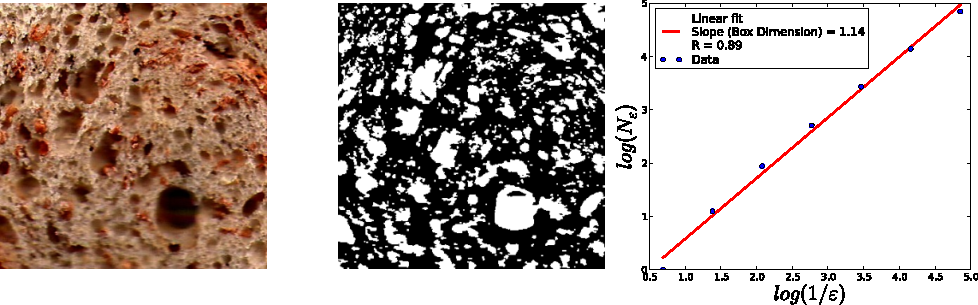
\includegraphics{dimensionbox}
\caption{Box dimension computation. A bread image (left) with its binarisation (centre) and its computed box dimension (right).}
\label{fig:fitbox}
\end{figure}

\begin{figure}[h!]
\centering
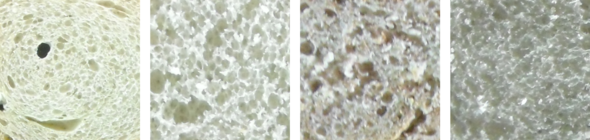
\includegraphics{pancamara}
\caption{Images from a digital camera.}
\label{fig:camera}
\end{figure}

\begin{figure}[h!]
\centering
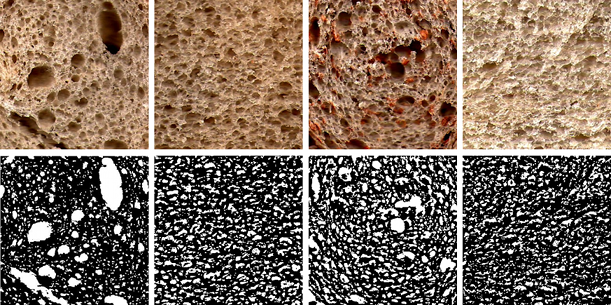
\includegraphics{binarizaciones}
\caption{Images from a scanner. {\em Baguette}, {\em sliced}, {\em bran} and {\em sandwich} bread types (top row) with their corresponding binarisations (bottom row).}
\label{fig:bread}
\end{figure}

\begin{figure}[h!]
\begin{centering}
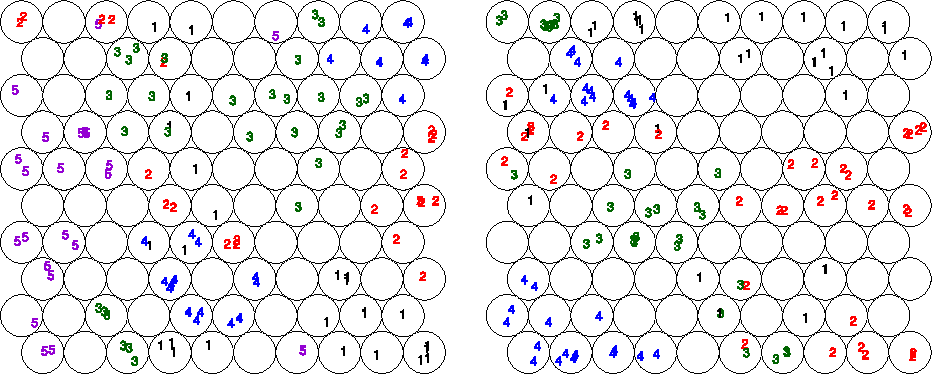
\includegraphics{SOM}
\caption{Self-organising maps (SOM). SOM of the bread and non-bread images (left) and SOM of the bread types only (right). $1$: {\em baguette}, $2$: {\em sliced}, $3$: {\em bran}, $4$: {\em sandwich}, $5$: {\em nonbread}.}
\label{fig:somfractal}
\end{centering}
\end{figure}

\begin{figure}[h!]
\centering
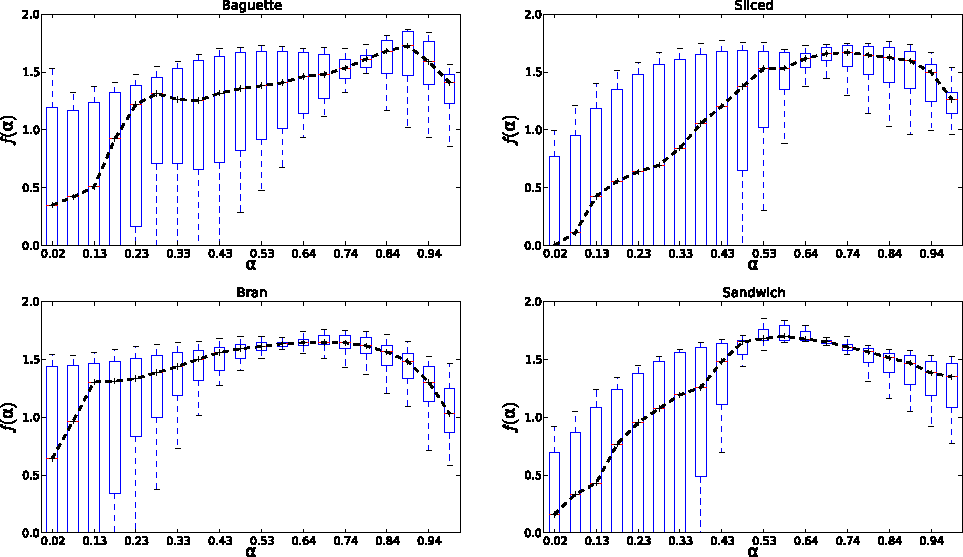
\includegraphics{boxplots}
\caption{Boxplots of the four different bread types. The FD medians are joined by a dashed line. Top: {\em baguette} (left), {\em sliced} (right), bottom: {\em bran} (left), {\em sandwich} (right).}
\label{fig:boxplotsMFS}
\end{figure}

\begin{figure}[h!]
\centering
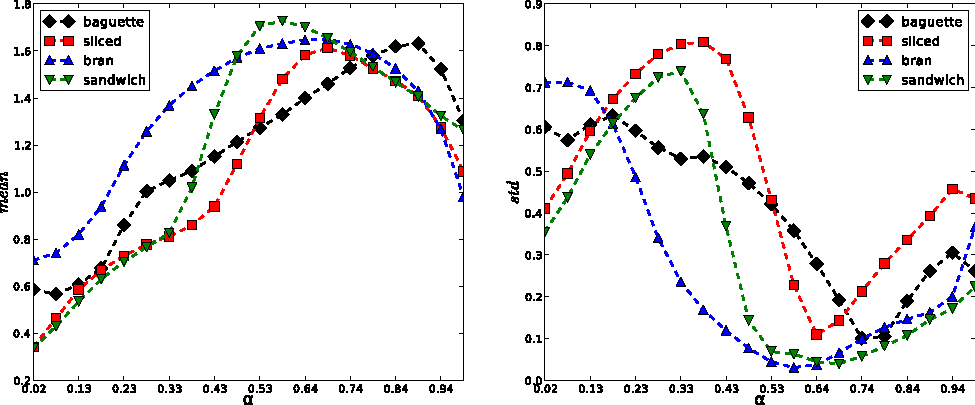
\includegraphics{panstd}
\caption{Mean MFS and standard deviations of the FDs for the four different bread types. Left: mean MFS, right: standard deviations.}
\label{fig:meansMFS}
\end{figure}


\begin{figure}[h!]
\centering
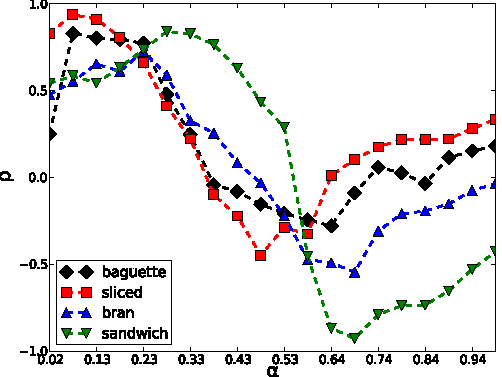
\includegraphics{VF}
\caption{Spearman correlation coefficients for the FDs and the void fraction of the scanned samples.}
\label{fig:corrVF}
\end{figure}

\begin{figure}[h!]
\centering
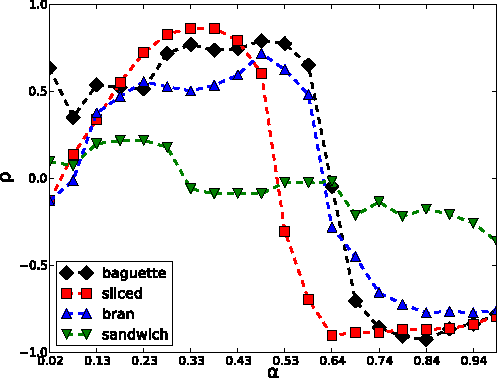
\includegraphics{MCA}
\caption{Spearman correlation coefficients for the FDs and the mean cell area. (In $[mm^{2}]$, scanned samples).}
\label{fig:corrMCA}
\end{figure}

\begin{figure}[h!]
\centering
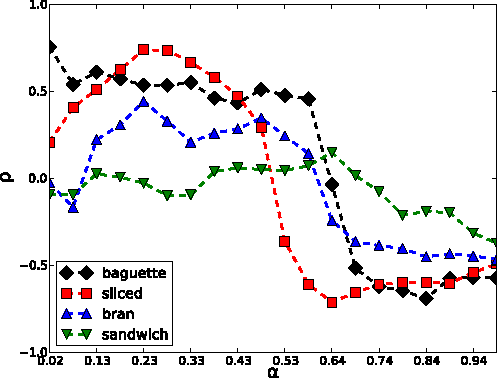
\includegraphics{stMCA}
\caption{Spearman correlation coefficients for the FDs and the standard deviation of the mean cell area. (In $[mm^{2}]$, scanned samples).}
\label{fig:corrMCAstdev}
\end{figure}




\begin{table}[h!]
% table caption is above the table
\caption{Bread crumb classification results with different number of FDs for the MFS and different classifiers.}
\label{tab:number}       % Give a unique label
% For LaTeX tables use
\begin{tabular}{lllll}
\hline\noalign{\smallskip}
\#FDs & 10  & 20 & 30 \\
\noalign{\smallskip}\hline\noalign{\smallskip}
SVM & \textbf{96\%} & 94.5\% & 95.5\% \\
RF  & 91.5\% & \textbf{93.5\%} & 93\% \\
NN & 88.5\% & \textbf{90.5\%} & 90\% \\
\noalign{\smallskip}\hline
\end{tabular}
\end{table}


\begin{table}[h!]
% table caption is above the table
\caption{Bread crumb classification results using different combinations of the MFS and different classifiers.}
\label{tab:mfs}       % Give a unique label
% For LaTeX tables use
\begin{tabular}{lllll}
\hline\noalign{\smallskip}
Method & MFS & MFS+L & MFS+G & CIELab  \\
\noalign{\smallskip}\hline\noalign{\smallskip}
SVM & 94.5\% & 95.5\% & \textbf{97.5\%} & \textbf{97.5\%} \\
RF  & 93.5\% & \textbf{96\%} & 95\% & \textbf{96\%} \\
NN & 90.5\% & 90\% & 87\% & \textbf{92\%} \\
\noalign{\smallskip}\hline
\#FDs & 20 & 40 & 40 & 60 \\
\hline
\end{tabular}
\end{table}

\begin{table}[h!]
% table caption is above the table
\caption{Bread crumb classification results for different state-of-the-art features and different classifiers.}
\label{tab:other}       % Give a unique label
% For LaTeX tables use
\begin{tabular}{llllll}
\hline\noalign{\smallskip}
Method & Haralick & Lbp & SIFT\\ % & Zernicke
\noalign{\smallskip}\hline\noalign{\smallskip}
SVM & 94\% & 78.5\% & \textbf{96.5\%} \\ % & 55 
RF  & 91\% & 71.5\% & \textbf{92\%} \\ % & 58 
NN & 79\% & 70\% & \textbf{86\%} \\ % & 48.5 
\noalign{\smallskip}\hline
\#FDs & 13 & 36 & 128 \\
\hline
\end{tabular}
\end{table}

\begin{table}[h!]
% table caption is above the table
\caption{Confusion Matrix for the best results (CIELab method, using the SVM classifier).}
\label{tab:confusionmatrix}       % Give a unique label
% For LaTeX tables use
\begin{tabular}{llllll}
\hline\noalign{\smallskip}
Clase&{\em baguette} & {\em lactal} & {\em salvado} &{\em sandwich}&{\em no-pan} \\
\noalign{\smallskip}\hline\noalign{\smallskip}
{\em baguette} & 39& 1 &1 &0 &0 \\
{\em lactal} & 0& 38 &0 &0 &0  \\
{\em salvado} & 0& 0 &39 &1 &0  \\
{\em sandwich} & 1& 1 &0 &39 &0  \\
{\em no-pan} & 0& 0 &0 &0 &40  \\
\hline
\end{tabular}
\end{table}


\subsection{Correlación entre Dimensiones Fractales y Características de la Miga de Pan.}

\section{Validación de Imágenes Sintéticas de Pan}

This section is included for the sole purpose of having a more objective assessment of our model's quality, apart from what subjective inspection may indicate. 
We validated our model using multifractal features, in particular, the multifractal spectrum method, that is widely used for texture analysis in computer vision and pattern analysis.
Fractal Dimensions (FD) can be used to characterize key image features using just a few parameters. 
Different FDs capture different features, {\em e.g.}, porosity, rugosity, etc.
Multifractal theory has also been used for image feature description, but not much in bread characterization. 
A few previous studies show fractal bread characterizations using several FDs \cite{Gonzales2008,Baravalle2012}. 
There are two main classes of multifractal spectra: generalized multifractal dimensions ($D_{q}$) and Lipschitz-H\"older exponents ($f(\alpha)$). 
The latter representation boosts the performance in classification tasks.

The generalized multifractal dimensions can be computed in several ways, of which the Sandbox multifractal method \cite{Tel1989} aims to compute the dimensions using the mean value in a set of randomly distributed points belonging to the structure \cite{Debartolo2004}. 
The generalized multifractal dimension of order $q$ with the sandbox method is defined as:

 \begin{align*}
D_{q\ne 1}^{sb} &= \frac{1}{q-1} \lim_{R \rightarrow 0}{
\frac{ln   { \left\langle  (M(R)/M_{0})^{q-1} \right\rangle   }}
{ln {(R/L)}       }},\\
D_{q=1}^{sb} &= \lim_{R \rightarrow 0}{
\frac{ \left\langle ln   { (M(R)/M_{0})  }  \right\rangle}
{ln {(R/L)}       }},
\end{align*}
%
where $M_{0}$ is the white pixel-count in the image binarization and  $M(R)$ is the number of points belonging to the structure in a circle of radius $R$ centered at a point in the structure. 
When $q\ne1$, we compute the limit as the slope of the linear fit of the values $ln(R/L)$ vs. $ ln  \left\langle  { (M(R)/M_{0})^{q-1} }  \right\rangle$, for $R$ in $[R_{min}, R_{max}]$, where $ \left\langle \cdot  \right\rangle$ denotes mean value over sampled points. 
The proceeding is similar when $q=1$. 
Computing the value for different $q \in [Q_{\min},Q_{\max}]$  we obtain the sandbox spectrum. %We will apply the sandbox approach to characterize real and synthetic bread binarizations.

This kind of analysis is reported to be the most adequate for geometrical and texture feature analysis~\cite{Gonzales2008,Baravalle2012}, so we applied it to $10$ binarized scanned real bread crumb images of the {\em baguette} bread type, and $10$ synthetic images produced using our pipeline, after the baking step, obtaining $20$ feature vectors.
We then separated each class and we computed boxplots for the two classes.
Actual bread crumbs were manually segmented to prevent errors from automatic segmentation as in \cite{Bosch2011}.
The model has $5$ parameters:

\begin{align*}
N &= \frac{k}{r^{d}},\\ r &= v_{min}+step*j, j \in [0,\frac{v_{max}}{step}],
\end{align*}
$k,d,v_{min},v_{max}$ and $step$ that controls bubble generation in the proving stage.
To compute the sandbox spectrum of each image, we used $1000$ different random points to ensure stability in the resulting spectrum.

We implemented an automated search in parameter space defining an error metric: 
\begin{equation*}
Error = \displaystyle \sum abs(means_{real}-means_{synthetic}),
\end{equation*}
and we found that the following parameters produce the lowest error:
\begin{align*}
k &= 0.07 \frac{N^{3}}{20} ,\\
d &=2.78,\\
v_{min} &=2,\\
v_{max} &=20.\\
step &=1,
\end{align*}
where $N$ is the proving volume dimensions in each spatial coordinate (we chose $N = 512$). 
The accumulated error in medians is $\sim 0.21$ meaning a mean error of $0.21/21 \sim 0.01$ in each dimension.
Fig.~\ref{bestboxplot} shows boxplots of real and synthetic breads with the medians for each dimension joined by dashed lines.
When $q < 0$ dimensions have a higher dispersion, since the method approximates these dimensions less accurately.
The figure shows almost identical spectra for real and synthetic breads. Fig.~\ref{realbin} and Fig.~\ref{best} show an example of real and synthetic binarizations for these parameters.


\begin{figure}[!ht]
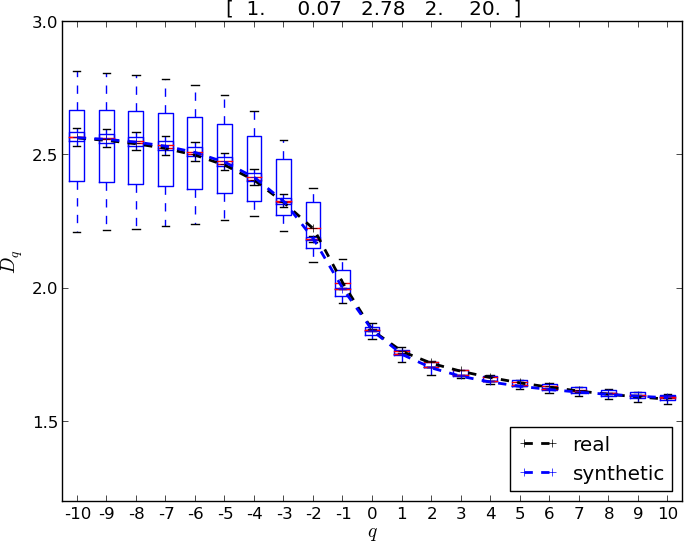
\includegraphics[width=9cm]{figures/bestboxplot}
\caption{Best fitting parameters for the {\em baguette} bread type. The total error in medians is $\sim 0.21$.}
\label{bestboxplot}
\end{figure}

\begin{figure}[!ht]
\begin{center}
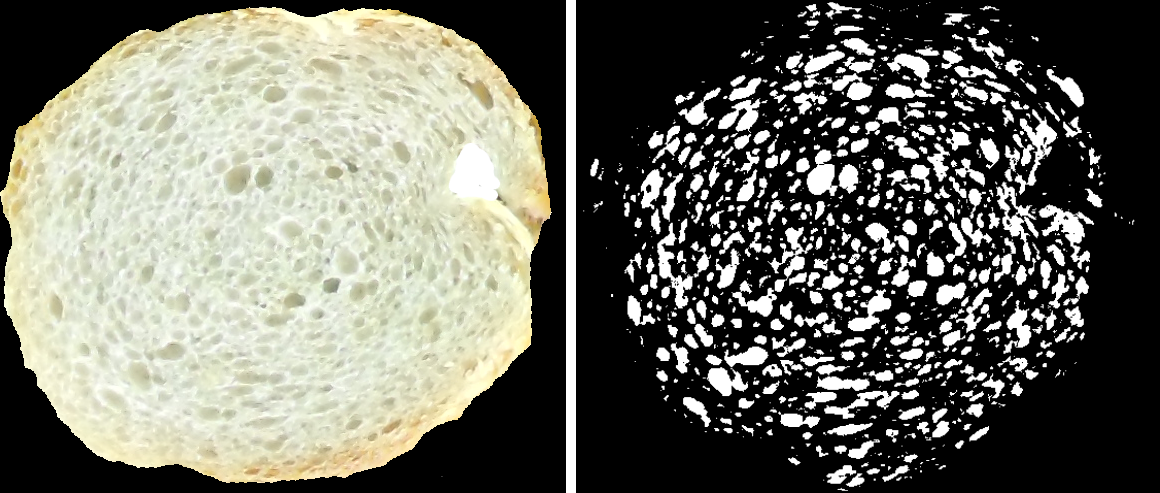
\includegraphics[width=9cm]{figures/realbin}
\caption{ Real {\em baguette} bread and binarization example.}
\label{realbin}
\end{center}
\end{figure}

\begin{figure}[!ht]
\begin{center}
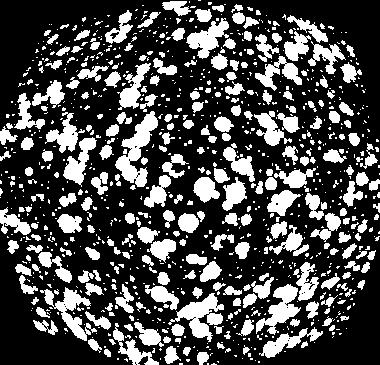
\includegraphics[width=6cm]{figures/best}
\caption{Model distribution example showing similar multifractal features to the {\em baguette} real bread type.}
\label{best}
\end{center}
\end{figure}

Also, we found parameters for a home-baked bread type using the same search:

\begin{align*}
k &= 0.69 \frac{N^{3}}{20} ,\\
d &=5.6,\\
v_{min} &=1,\\
v_{max} &=24.\\
step &=1,
\end{align*}

Fig.~\ref{bestboxplot2} shows boxplots of real and synthetic breads for this bread type. Fig.~\ref{realbin2} and  Fig.~\ref{best2} show an example of real and synthetic binarizations for these parameters and bread type. 


\begin{figure}[!ht]
\includegraphics[width=9cm]{figures/bestboxplot2}
\caption{Best fitting parameters for a home-baked bread type. The total error in medians is $\sim 0.88$.}
\label{bestboxplot2}
\end{figure}

\begin{figure}[!ht]
\begin{center}
\includegraphics[width=9cm]{figures/realbin2}
\caption{ Real home-baked bread and binarization example.}
\label{realbin2}
\end{center}
\end{figure}

\begin{figure}[!ht]
\begin{center}
\includegraphics[width=6cm]{figures/best2}
\caption{Model distribution example showing similar multifractal features to a home-baked real bread type.}
\label{best2}
\end{center}
\end{figure}


%We apply the sandbox multifractal method to study the geometry we obtained after the deformation step. This method is best suited for geometrical measurements than other multifractal approaches.

%We apply the sandbox method to $10$ binarised real bread crumb images of the {\em baguette} bread type that we captured with a digital scanner and $10$ syhthetic images produced using our pipeline, after the deformation step, obtaining $20$ feature vectors. Then we separate each class and we compute boxplots for the two classes. We manually segmented real bread crumbs to prevent automatic segmentation errors as in \cite{Bosch2011}. The model has $5$ parameters:


%\begin{align}
%N_{spheres} &= \frac{k}{r^{d}},\\ r &= v_{min}+step*j, j \in [0,\frac{v_{max}}{step}]
%\end{align}
%$k,d,v_{min},v_{max}$ and $step$ that controls bubble's generation in the proving stage. %To compute the sandbox spectrum of each image, we used $5000$ different random points to ensure stability in the resulting spectrum.

%We implemented an automated search in parameter space and we found that the following parameters produce the lowest error:

%\begin{align*}
%k &= 0.07 \frac{N_{x}\times N_{y}\times N_{z}}{20} ,\\
%d &=2.78,\\
%v_{min} &=2,\\
%v_{max} &=20.\\
%step &=1,
%\end{align*}
%\noindent where $N_{x}$, $N_{y}$ and $N_{z}$ are the proving volume dimensions in each spatial coordinate (we chose $(N_{x},N_{y},N_{z}) = (760,760,100)$). The accumulated error in medians is $\sim 0.21$ meaning a mean error of $0.21/21 \sim 0.01$  in each dimension. We compute this error as:

%\begin{equation}
%Error = \displaystyle \sum abs(means_{real}-means_{synthetic}).
%\end{equation}
%Fig.~\ref{bestboxplot} shows boxplots of real and synthetic breads with the medians for each dimension joined by dashed lines. When $q < 0$ dimensions have a higher dispersion, since the method approximates these dimensions less accurately. The figure shows almost identical spectra for real and synthetic breads.  Fig.~\ref{realbin} and  Fig.~\ref{bestwarp} show an example of real and synthetic binarisations for these parameters.

%\begin{figure}[!ht]
%\includegraphics[scale=0.5]{bestboxplot.png}
%\caption{Best fitting parameters. The total error in medians is $\sim 0.21$.}
%\label{bestboxplot}
%\end{figure}

%\begin{figure}[!ht]
%\begin{center}
%\includegraphics[scale=0.2]{realbin.png}
%\caption{ Real bread and binarisation example.}
%\label{realbin}
%\end{center}
%\end{figure}

%\begin{figure}[!ht]
%\begin{center}
%\includegraphics[scale=0.4]{bestwarp.png}
%\caption{Model distribution example showing similar multifractal features to real breads .}
%\label{bestwarp}
%\end{center}
%\end{figure}


%Automated searchs in parameter space may be useful to automatically match other bread types and materials.

%\section{Resultados}
\section{Discusi\'on y Conclusiones}
This method allows to approximate the geometry of any real bread crumb, by 
extracting parameters in order to accurately simulate it.
Bubble distributions under our model were shown to be statistically coincident to real bread, according to multifractal methods.
The sandbox analysis method produced very similar fractal features both with our synthetic images and with images of real bread crumbs.
Two bread types were tested: a home-baked and the {\em baguette } bread types.
The home-baked multifractal spectrum was more difficult to fit ({\em i.e.}, the errors were larger than those of the {\em baguette} bread type), but notwithstanding this the final bubble distribution was adequate for emulating this bread type.
Multifractal spectra showed higher dispersion in the negative dimensions ($q < 0$), which means that at finer geometric scales it is more difficult to characterize the statistical distribution, due to the image resolution.
A more detailed link between bread crumb physical features (coarseness, porosity) and multifractal features may be useful for designing better procedural models \cite{Baravalle2012}.
Multifractal image analysis was used to validate the model.
The statistical similarity between $2D$ cuts in our results and of real-word bread slices suggests that it may be suitable for applications in $3D$ engines, serious games \cite{Susi2007} and photorealistic rendering. 


 \cleardoublepage
\chapter{Conclusiones y Trabajos a Futuro}
\section{Conclusiones}
\section{Trabajos a Futuro}

 \cleardoublepage

\appendix
\chapter{Programación de Placas Gráficas}
\section{Introduccion a la historia del Shader Programable}
\section{Paralelismo}
\section{Libreras de computo general (GPGPU): OpenCL-CUDA}
\section{Comparación GPU-CPU}
\section{Fractales y Multifractales en Computación Gráfica}
\section{Aplicaciones}
 \cleardoublepage


%Otros apéndices (detalles matemáticos, aspectos tecnológicos del pan, etc.)

\cleardoublepage
\addcontentsline{toc}{chapter}{Bibliografía}
\bibliographystyle{unsrt}
\bibliography{bib}


\end{document}
